

\section{Internet Protocol (IP) version 4}

\subsection*{Introduzione}
\begin{figure}[h!]
    \begin{minipage}{0.45\textwidth}
        \centering
        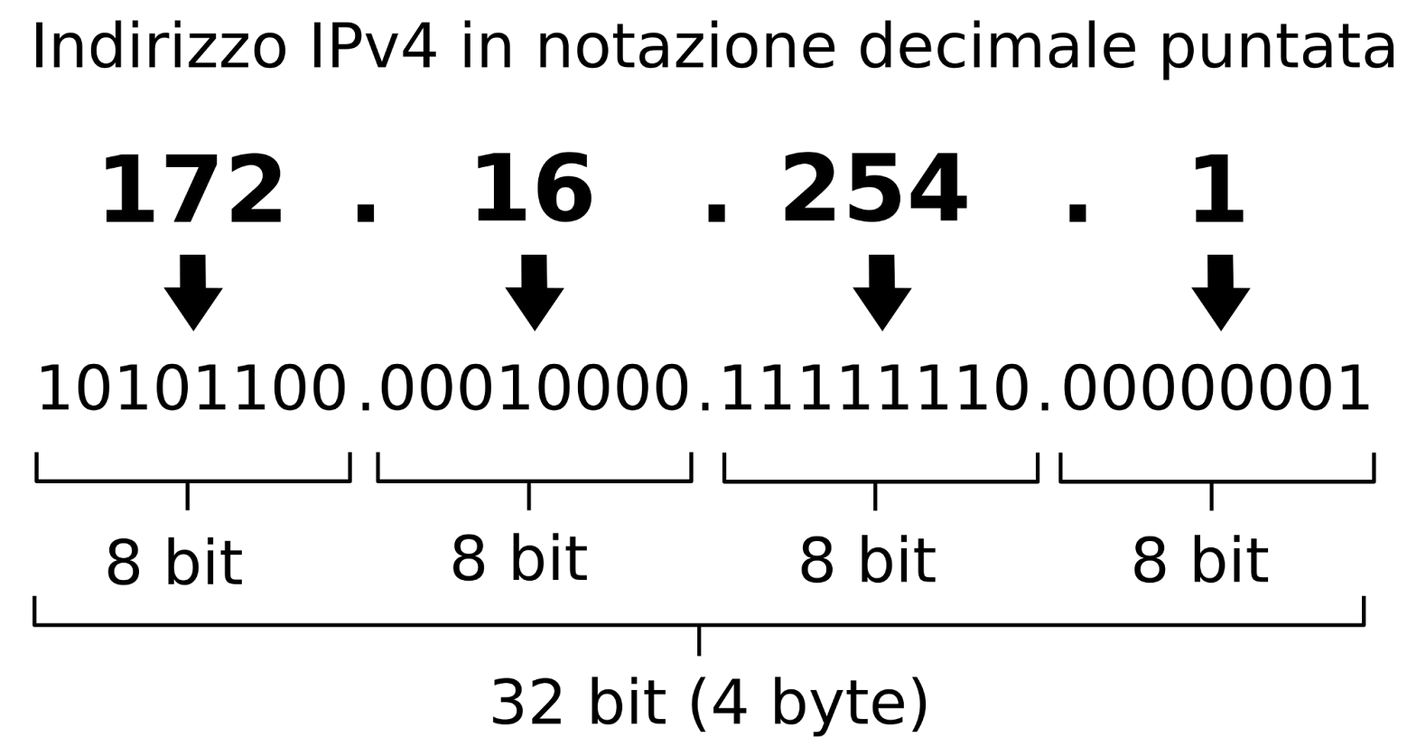
\includegraphics[width=0.95\textwidth]{images/indirizzoip.png}
        \caption{Struttura di un indirizzo IP}
        \label{fig:indirizzoip}
    \end{minipage}\hfill
    \begin{minipage}{0.52\textwidth}
        Al livello 3 ci preoccupiamo di trovare la strada migliore per raggiungere il destinatario.

        IPv4 è il protocollo di rete più diffuso al mondo, IP instrada i pacchetti immessi nella rete, ogni nodo in rete ha indirizzo ip.

        Ogni pdu(pacchetto) contiene gli indirizzi IP del host mittente e destinatario.
        
        IP è connectionless, ad inoltrare i pacchetti(datagram) sono i router, lo fanno attraverso algoritmi di routing(leggendo l’header del pacchetto). 

        Ip è inoltre “best-effort”, ossia fa del suo meglio, non garantisce affidabilità massima o ottimale.

        Gli indirizzi ip sono da 32 bit(4 numeri decimali compresi tra 0 e 255):
    \end{minipage}
\end{figure}

Gli host che appartengono alla stessa rete hanno in comune il livello fisico,
un dominio di broadcast è un insieme di computer di una stessa rete(stesso indirizzo ip di rete), esempio rete di casa(collegandoci al router di casa è possibile inviare un messaggio broadcast che arriverà a tutti i dispositivi che fanno parte della rete IP).
Le porte del router vengono chiamate interfacce, ogni interfaccia corrisponde ad un host;
ogni rete ha un indirizzo IP di rete.

\begin{figure}[h!]
    \centering
    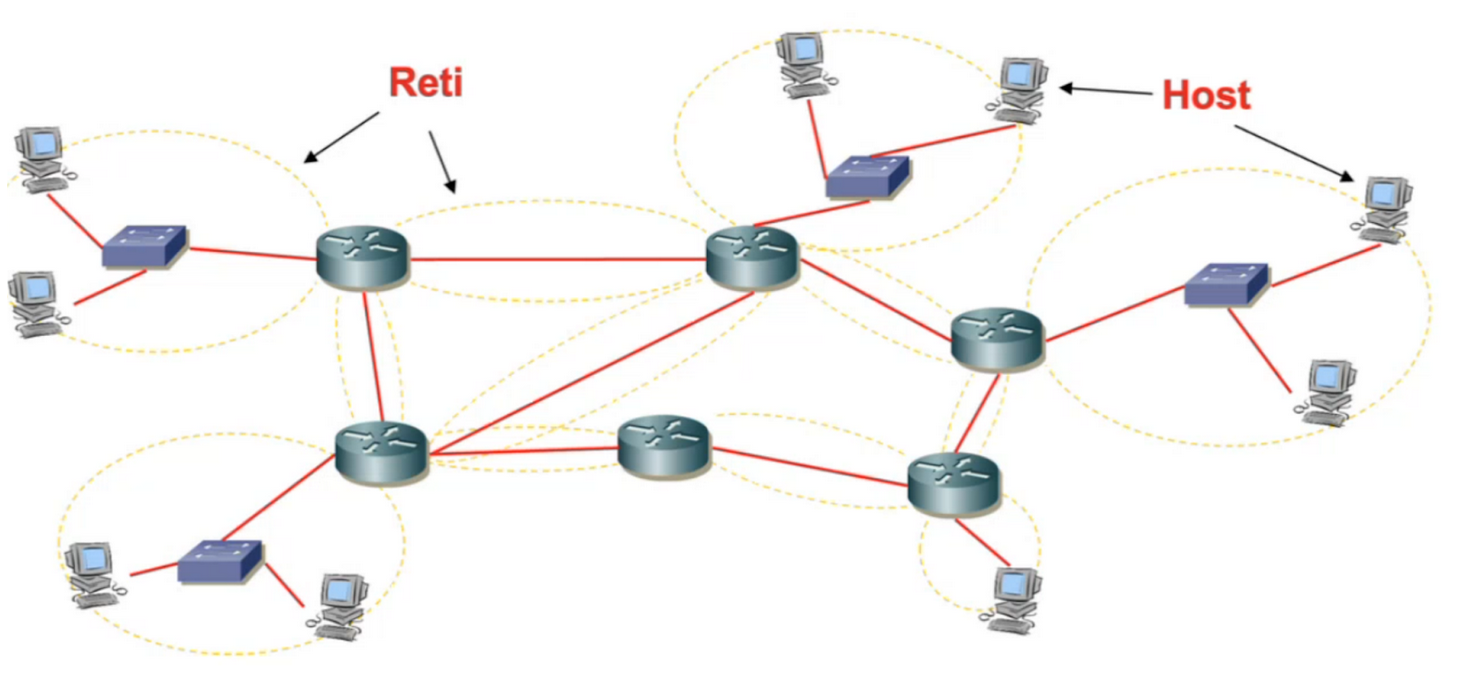
\includegraphics[width=0.59\textwidth]{images/reteipbase.png}
    \caption{Esempio di rete IP di base}
    \label{fig:reteipbase}
\end{figure}
\subsection{Datagramma IP}
I datagrams IP sono i pacchetti di dati che vengono inviati attraverso la rete utilizzando il protocollo IP. Ogni datagramma contiene un header e un payload. 
\begin{figure}[h!]
    \centering
    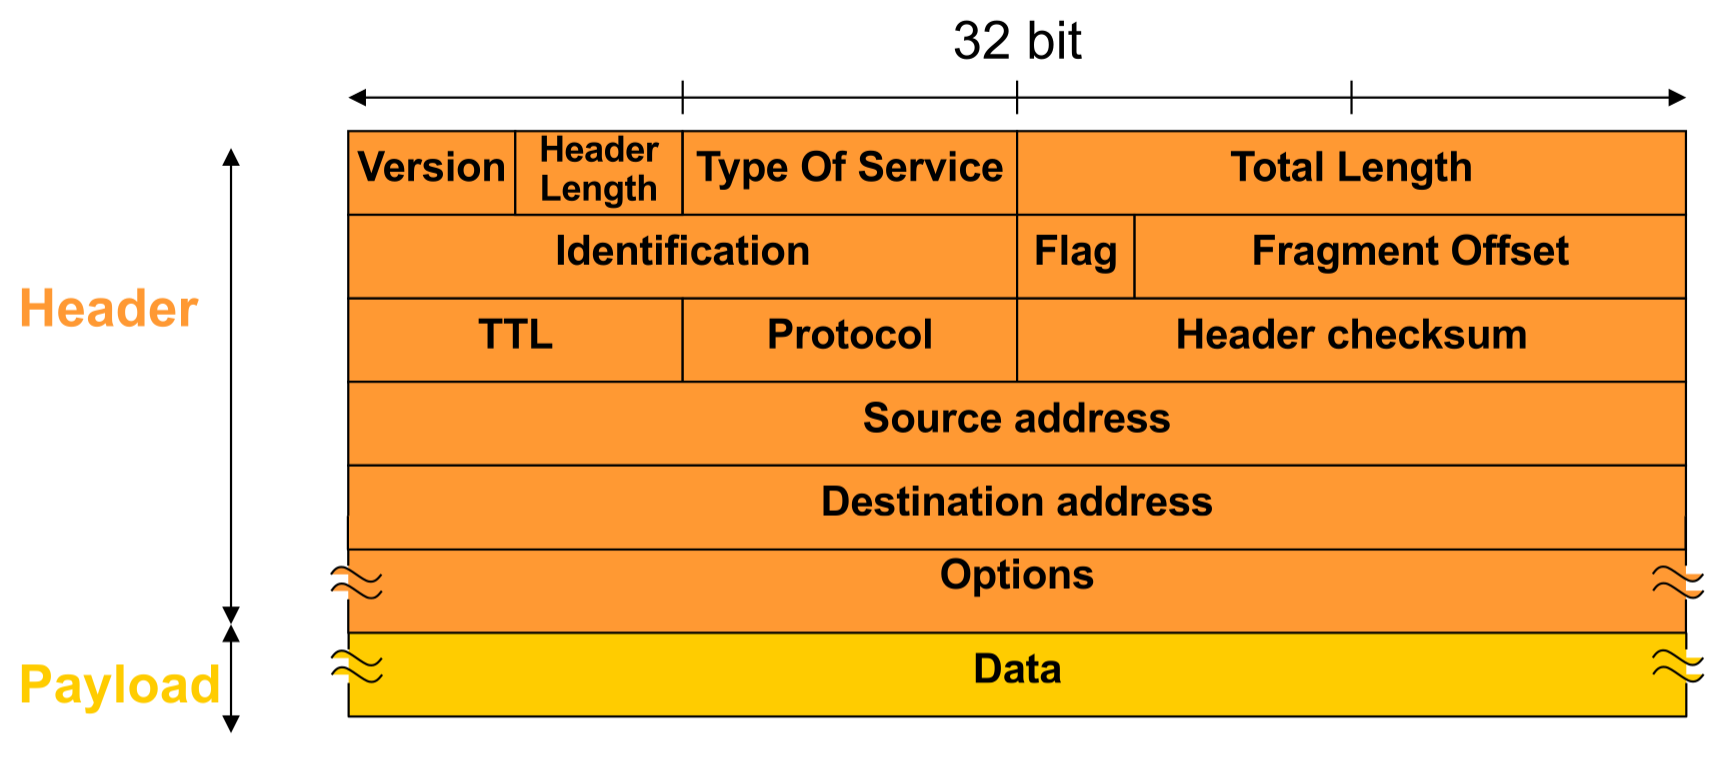
\includegraphics[width=0.9\textwidth]{images/datagrammaIP.png}
    \caption{Struttura di un datagramma IP}
    \label{fig:datagrammaIP}
\end{figure}

\begin{itemize}
    \item version: mi dice la versione del protocollo(IPv4 o IPv6) (è di 4 bit, mezzo byte)
    \item header legth: lunghezza del header (4 bit, mezzo byte), se voglio dire che l'header è lungo 5 posso scivere in questo campo 0101, che è 1 + 0 + 4 + 0
    \item type of service(TOS): (1 byte, 8 bit) distingue i tipi diversi di pacchetti, questo è utile nel momento in cui un router deve dare o no la precedenza a certi pacchetti, in base al tipo di servizio. esempio: precedenza al servizio x piuttosto che a y
    il TOS viene utilizzato per definire il liello di quality of service con cui trattare il pacchetto(primi 6 bit)(gli ultimi 2 servono ad evitare la congestione)
    
    \begin{figure}[h!]
        \centering
        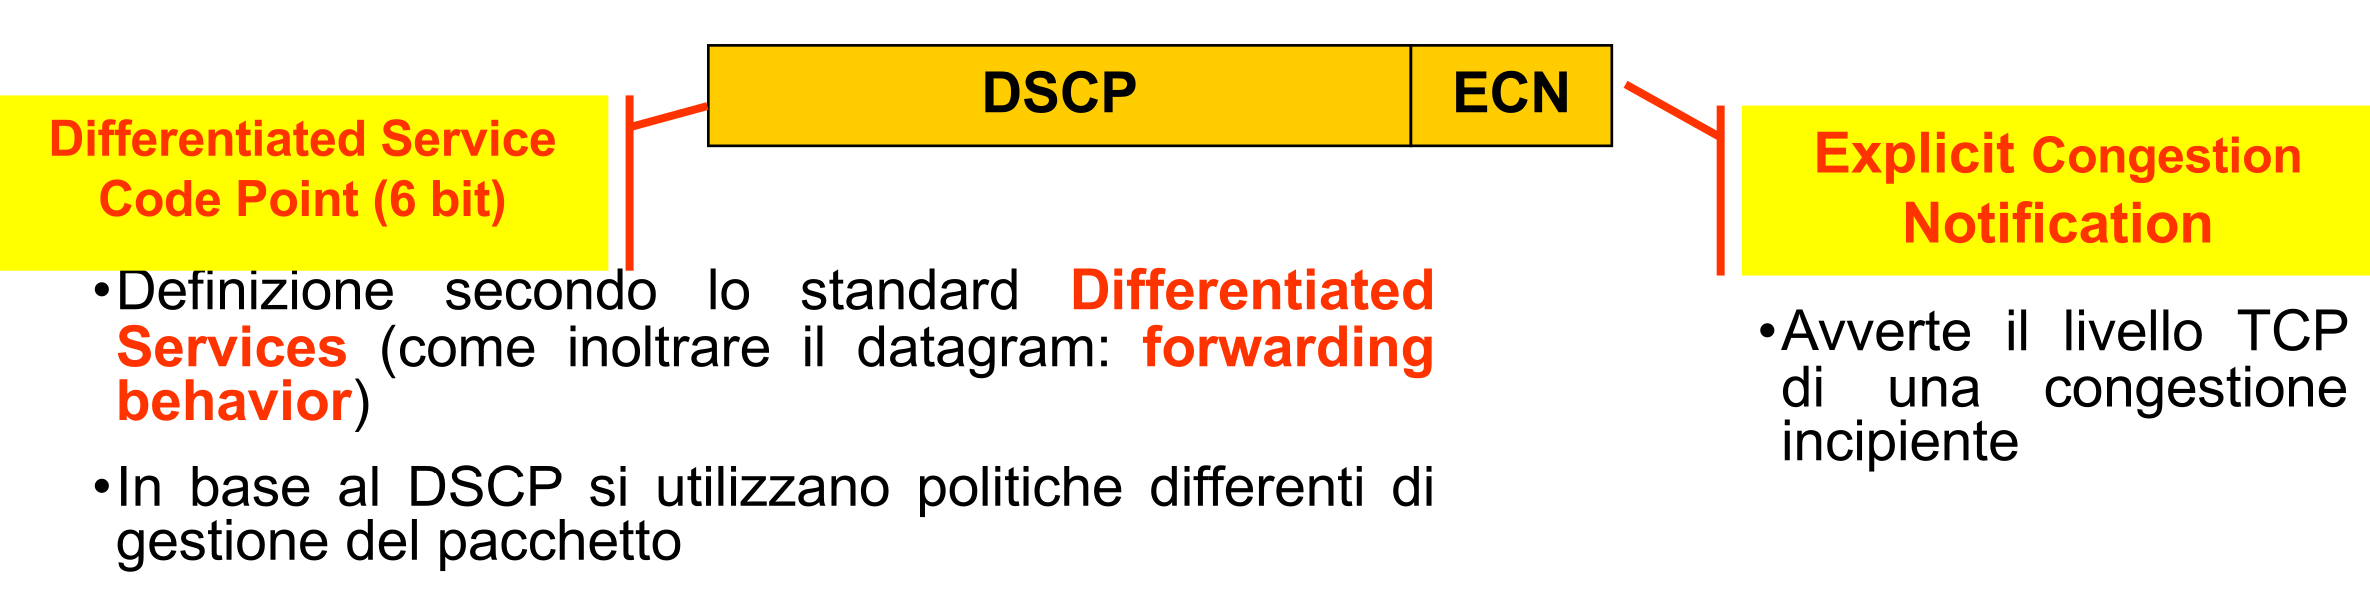
\includegraphics[width=1\textwidth]{images/tos.png}
        \caption{Campo Type of Service (ToS) nell'header IP}
        \label{fig:tos}
    \end{figure}

    \item total length:(16 bit) lunghezza del datagramma in byte(max 65535 byte)
    \item identification(16 bit) identifica in modo univoco un datagramma generato dal mittente, quindi anche se il pacchetto viene frammentato, i suoi “frammenti”, ossia altri pacchetti che contengono parte del payload iniziale, avranno lo stesso id. serve quindi a gestire la frammentazione dei pacchetti ip
    \item options: opzioni per il routing del pacchetto, è un campo poco usato per via del carico di elaborazione molto variabile
    \item data: è l'informazione da inviare
\end{itemize}
\newpage
\begin{itemize}
    \item flag(3 bit)
\end{itemize}
        \begin{figure}[h!]
            \begin{minipage}{0.55\textwidth}
                \raggedright
                 il primo bit non usato, il secondo bit è il flag DF (don't fragment: specifica che il router può frammentare il pacchetto o no), il terzo bit è il flag MF (more fragment: indica se il seguente datagramma è l'ultimo dei frammenti). Per utilizzare questi flag metto il valore del bit corrispondente al flag ad 1. Esempio: 010, 0 iniziale è indifferente, 1 indica il flag DF attivo, mentre lo 0 alla fine mi dice che non è MF, quindi che questo datagram è l'ultimo frammento.
            \end{minipage}\hfill
            \begin{minipage}{0.4\textwidth}
                \centering
                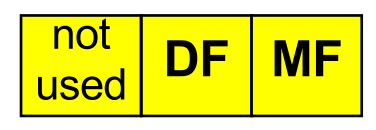
\includegraphics[width=\textwidth]{images/flagsIP.png}
                \caption{Campo Flags nell'header IP}
                \label{fig:flagsIP}
            \end{minipage}
        \end{figure}
\begin{itemize}
    \item fragment offset(13 bit) mi dice la posizione del frammento all'interno del pacchetto originario, lo spiazzamento. è espresso in multipli di 8 byte. 
\end{itemize}

    \begin{figure}[h!]
        \begin{minipage}{0.55\textwidth}
            \textbf{Frammentazione}: quando un datagramma IP deve attraversare una rete con una MTU (Maximum Transmission Unit) inferiore alla sua dimensione, viene suddiviso in frammenti più piccoli. Ogni frammento contiene parte dei dati originali e un header IP con informazioni per il riassemblaggio.

            Nella figura il pacchetto è grande 4000 byte(total length), in questo caso viene frammentato in 3 poichè la sua MTU vale 1500 byte , i frammenti condividono lo stesso id del pacchetto non frammentato.

            I frammenti devono avere un offset multiplo di 8.

            Solamente il primo frammento ha offset pari a 0, rappresenta la testa.
            Solamente l'ultimo frammento ha MF pari a 0 poichè sta ad indicare che quello è l'ultimo pezzo del pacchetto, la coda. CHIARIRE
        \end{minipage}\hfill
        \begin{minipage}{0.4\textwidth}
            \centering
            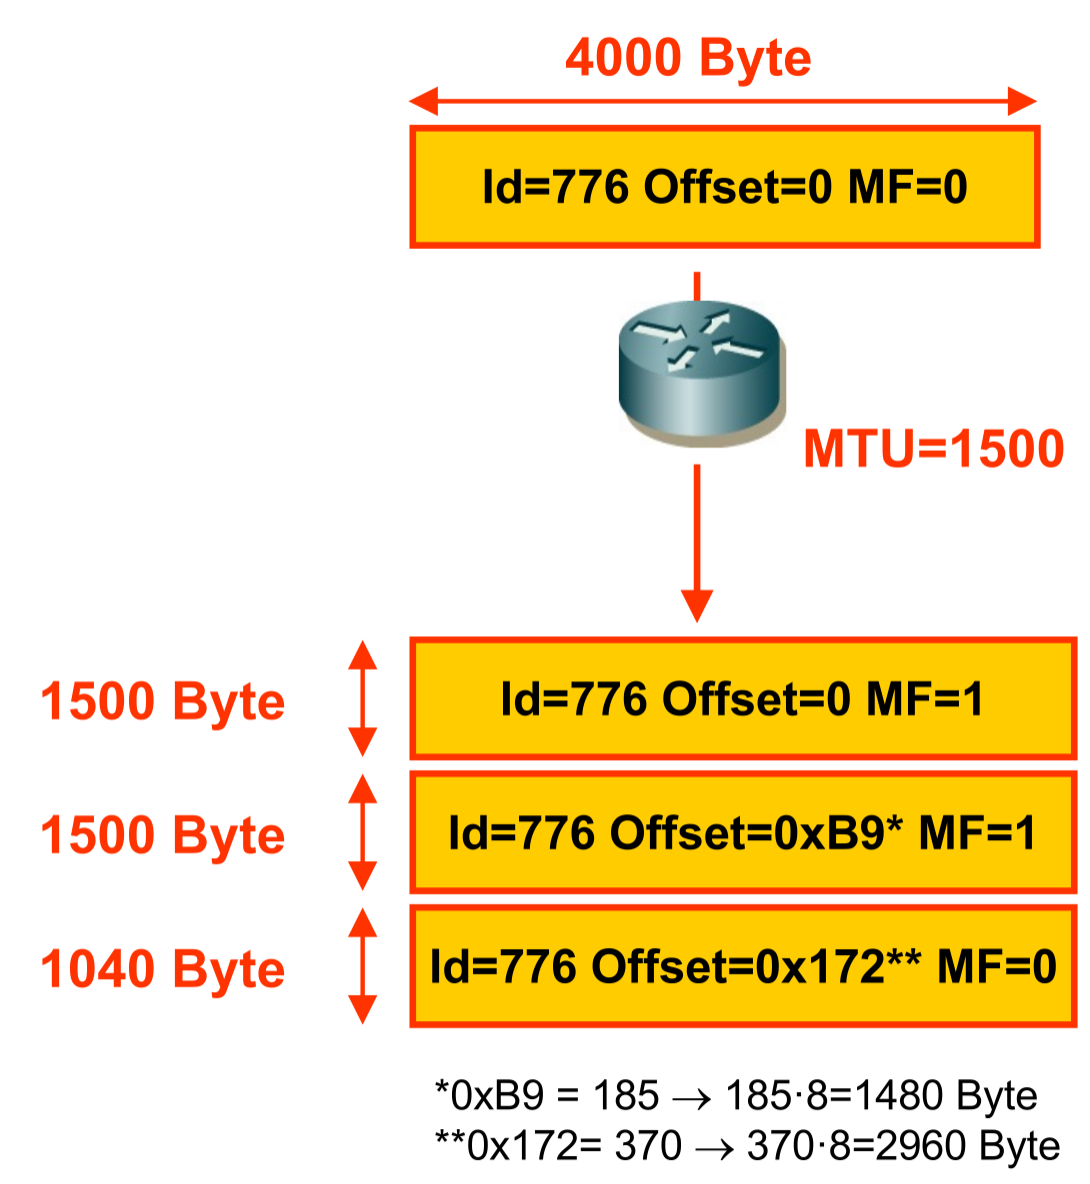
\includegraphics[width=\textwidth]{images/frammentazione.png}
            \caption{Esempio di frammentazione di un datagramma IP}
            \label{fig:frammentazioneIP}
        \end{minipage}
    \end{figure}

\begin{itemize}
    \item time to live(8 bit) evita il problema dei pacchetti che entrano in loop poichè non trovano il destinatario. è il tempo di vita del pacchetto, ogni router che riceve il pacchetto(ad ogni hop) decrementa il valore time to live, facendo così arriverà un punto in cui il time to live del pacchetto è stato decrementato fino a zero. quando arriva a 0 il datagram viene scartato. è un valore stabilito dal mittente(esempio 128)
    \item protocol(8 bit): contiene un numero che specifica il protocollo usato dalla PDU incapsulata dal datagram. esempio TCP = 6 . UDP = 17 $\rightarrow$ livello 4
    \item header checksum(16 bit): controlla i byte del header, è un controllo veloce su header. se c'è un errore sull'header allora il pacchetto viene scartato, come funziona? : somma 16 bit a 16 bit gli altri byte dell’header,fa la somma dell'eventuale resto e fa il complemento ad 1 del risultato.

Se non ci sono errori, la somma a 16 bit di tutti questi valori deve dare come risultato 0xFFFF (cioè tutti i bit a 1).

\item source/destination address: (32 bit) è l'indirizzo ip del mittente/destinatario

\end{itemize}

\subsubsection{Struttura indirizzo IP}
\begin{figure}[h!]
    \centering
    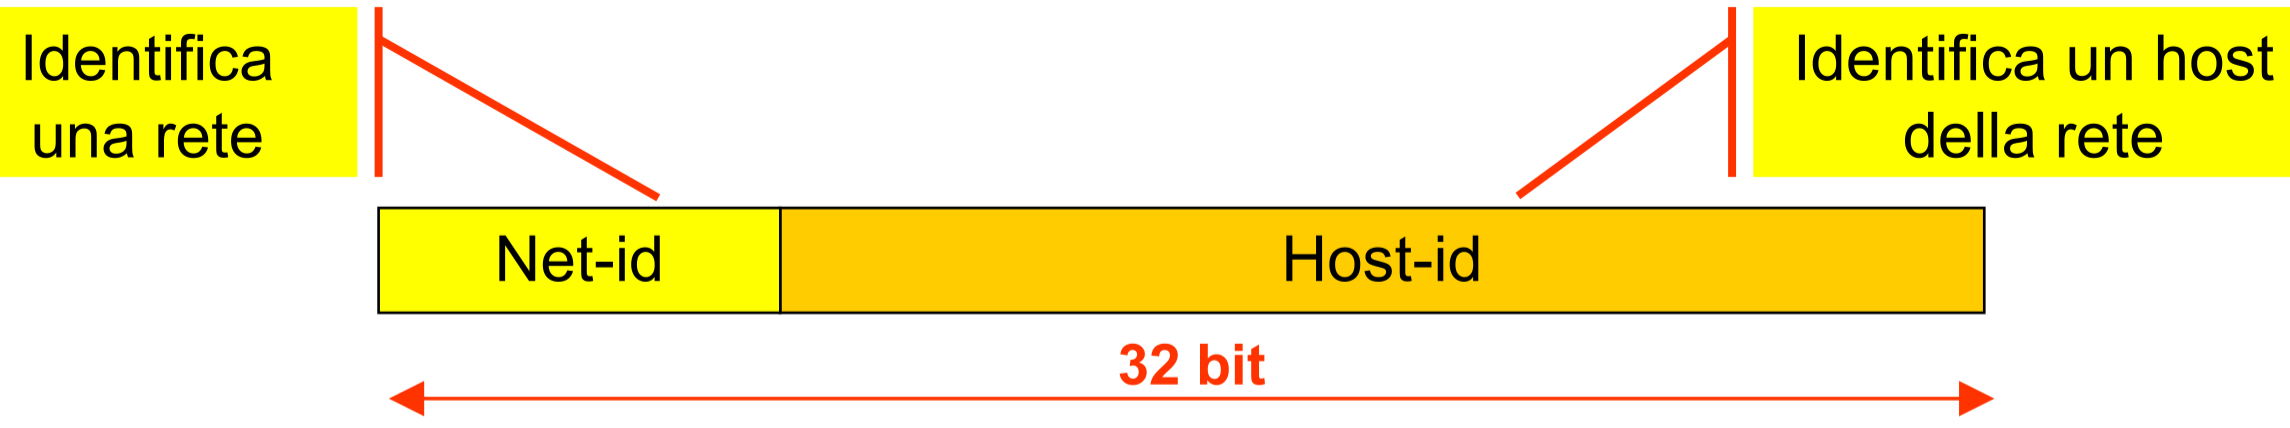
\includegraphics[width=0.8\textwidth]{images/strutturaIP.png}
    \caption{Struttura di un indirizzo IP: suddivisione in parte di rete e parte host}
    \label{fig:strutturaIP}
\end{figure}

Attualmente si utilizza l'indirizzamento classless CIDR (Classless Inter-Domain Routing), che permette di specificare la lunghezza della maschera di rete in bit.

L'assegnazione degli indirizzi è compito dell'Internet Assigned Number
Authority (IANA) gestita dall'ICANN (Internet Corporation for Assigned
Names and Numbers).

Ogni interfaccia (host) della rete IP ha un suo indirizzo.

\subsection{Indirizzo IP - classful}

\begin{figure}[h!]
    \centering
    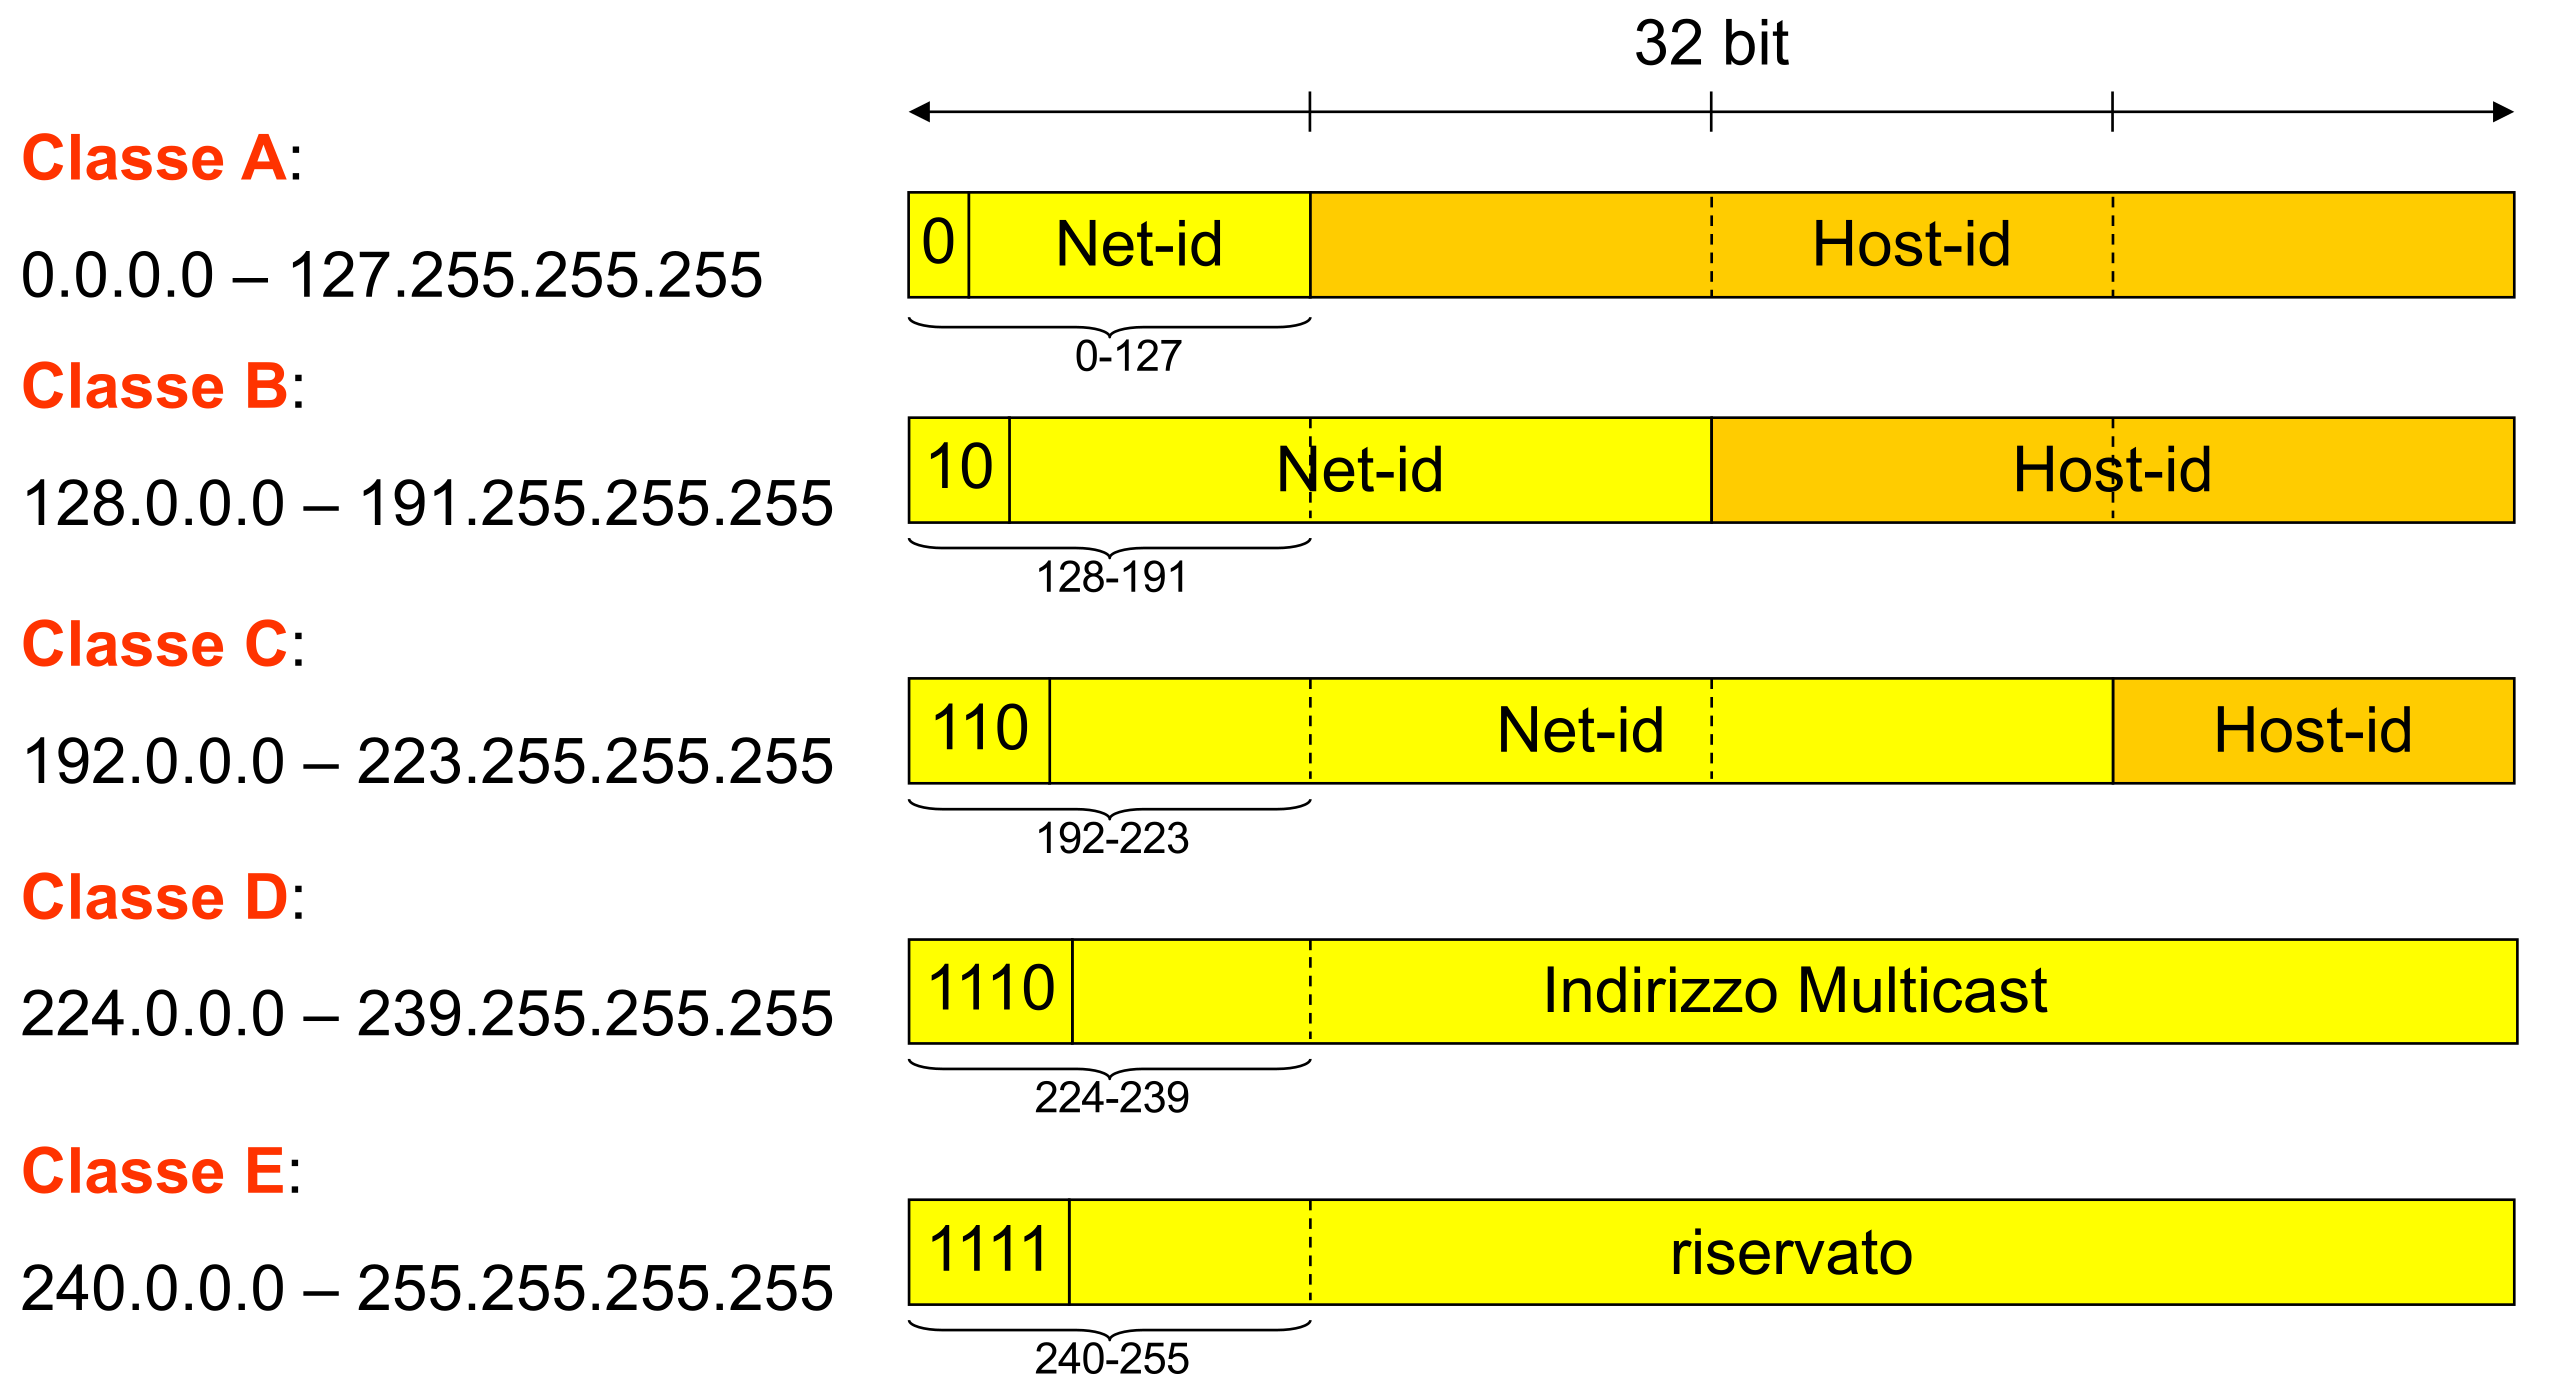
\includegraphics[width=1\textwidth]{images/classfulladdressing.png}
    \caption{Classful Addressing: suddivisione degli indirizzi IP in classi A, B, C, D, E}
    \label{fig:classfuladdressing}
\end{figure}

\subsection{Indirizzo IP - classless CIDR}

\begin{figure}[h!]
    \begin{minipage}{0.45\textwidth}
        \centering
        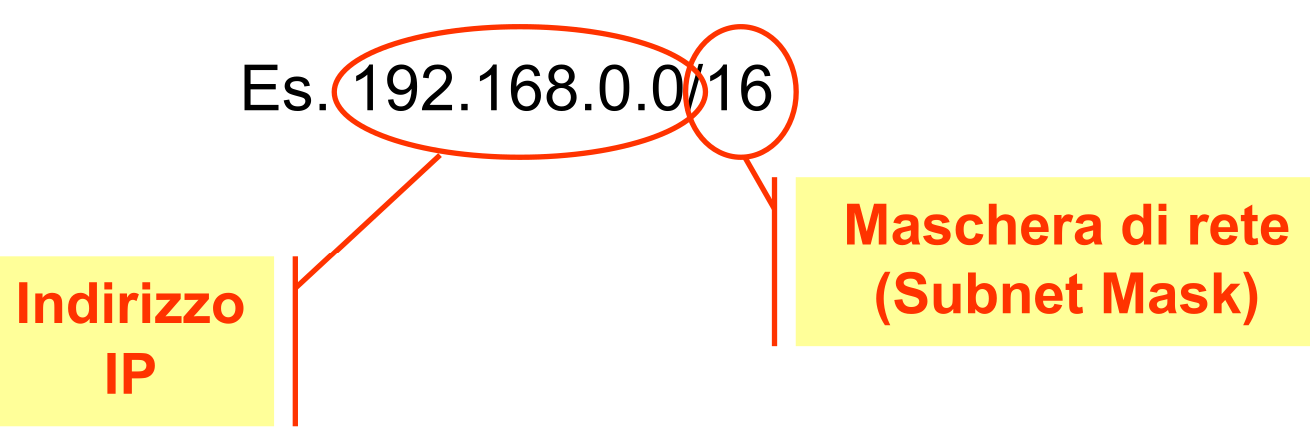
\includegraphics[width=0.95\textwidth]{images/mascheraIP.png}
        \caption{Esempio di maschera di rete (netmask) in notazione decimale e binaria}
        \label{fig:mascheraIP}
    \end{minipage}\hfill
    \begin{minipage}{0.52\textwidth}
        Il formato dell'indirizzo è del tipo \texttt{a.b.c.d/x} dove $x$ rappresenta la lunghezza della maschera di rete in bit.

        La maschera di rete permette di distinguere la parte di indirizzo relativa alla rete da quella relativa all'host. In notazione CIDR, la maschera viene indicata dopo una barra, ad esempio \texttt{192.168.1.0/24}.
    \end{minipage}
\end{figure}

%\paragraph{Riconoscere un indirizzo di rete e un indirizzo di host}

%Per riconoscere un indirizzo di rete e un indirizzo di host, si utilizza la maschera di rete. La maschera di rete è un numero che indica quanti bit dell'indirizzo IP sono dedicati alla parte di rete e quanti alla parte di host.

%\begin{itemize}
%    \item Un indirizzo di rete ha tutti zero nella parte di host.
%\end{itemize}
%\subsection{Subnetting}
%paragraph{Piggybacking}

%\subsection{Classificazione degli indirizzi IP}

%\subsubsection{Pubblici}
%\subsubsection{Privati}

%\subsubsection{Statici}
%\subsubsection{Dinamici}


%\subsection{Variable Length Subnet Mask (VLSM)}
%\subsection{Indirizzi IP speciali}

%\begin{figure}[h!]
%    \centering
%    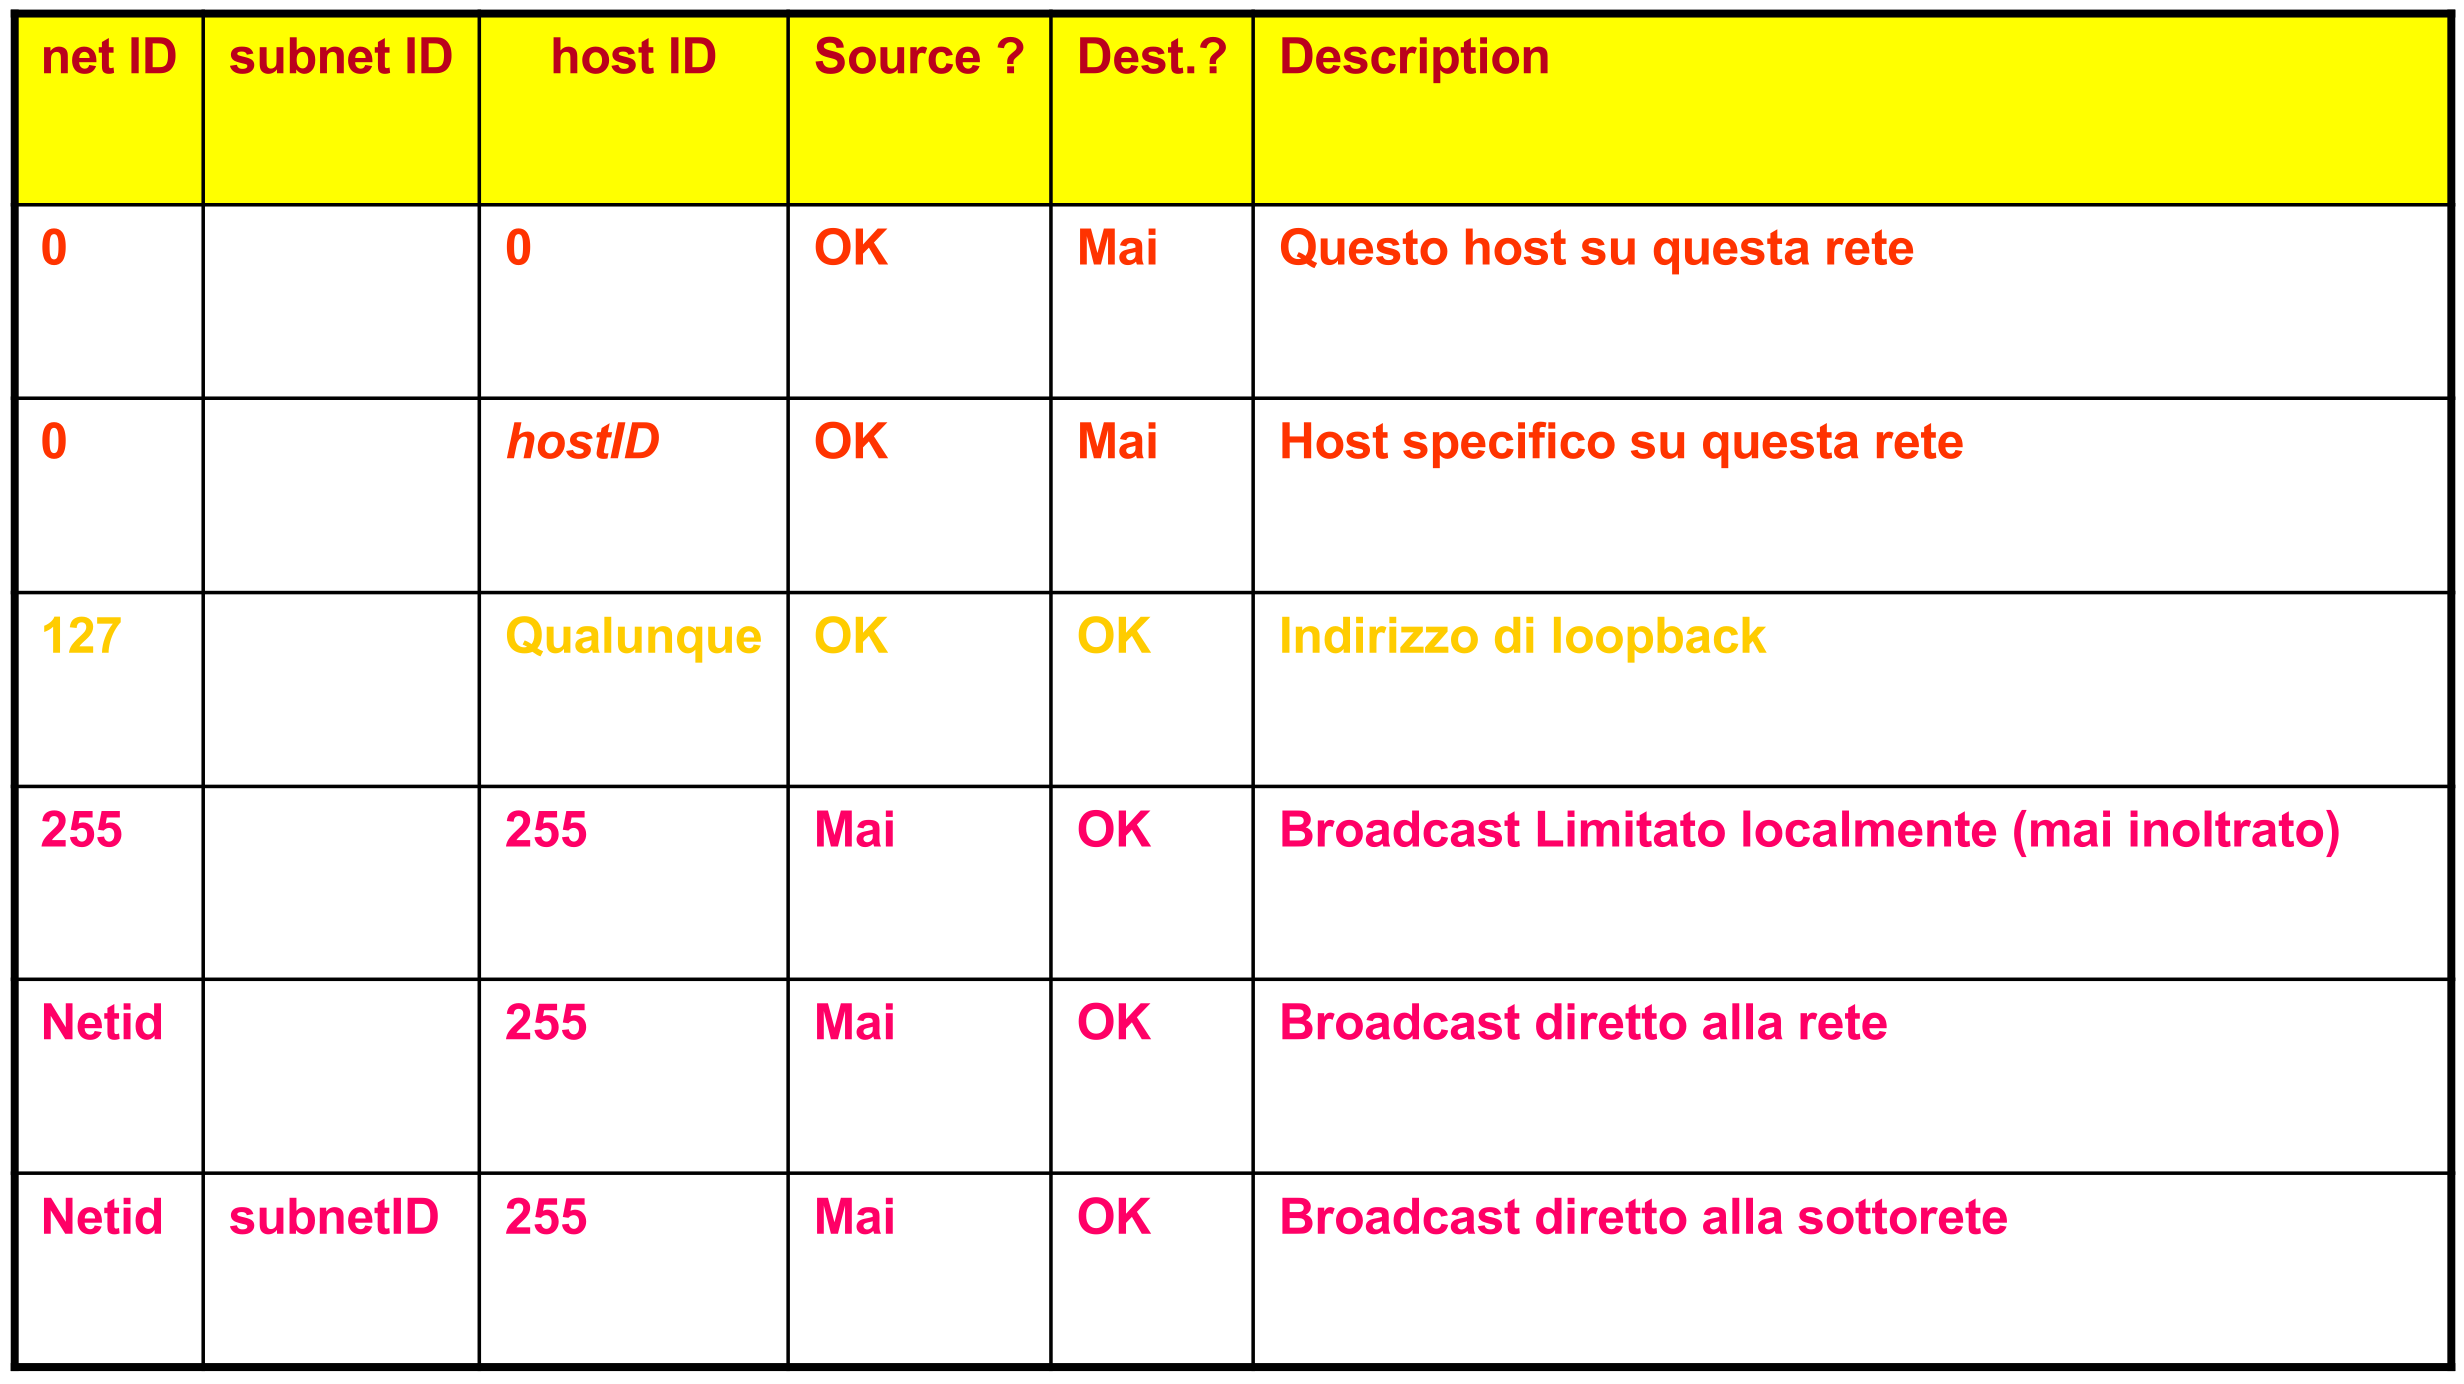
\includegraphics[width=1\textwidth]{images/indirizziipspeciali.png}
%    \caption{Indirizzi IP speciali}
%    \label{fig:indirizziipspeciali}
%\end{figure}


\newpage
\subsection{Address Resolution Protocol (ARP) - mappatura IP a MAC}
Con ARP si intende un protocollo di rete appartenente alla suite del protocollo internet (IP) versione 4 e operante a livello di accesso alla rete (livello collegamento se si considera nomenclatura ISO/OSI), il cui compito è fornire la "mappatura" tra l'indirizzo IP (32 bit - 4 byte) e l'indirizzo MAC (48 bit - 6 byte) corrispondente di un terminale in una rete locale ethernet.

Cos'è l'indirizzo MAC? 

Un indirizzo MAC (dove MAC sta per Media Access Control), detto anche "indirizzo fisico" o "indirizzo Ethernet", è un codice di 48 bit associato ad ogni dispositivo di rete che implementa lo standard Ethernet. Il suo scopo principale è quello di attribuire un'identità univoca a ciascuno dei nodi collegati ad uno stesso segmento di rete, consentendo quindi comunicazioni locali di tipo unicast. 

Al Livello 2 del modello ibrido, i pacchetti viaggiano attraverso il collegamento di più nodi, questi nodi sono caratterizzati da indirizzi fisici detti mac. 
Invece a livello tre l'indirizzo che possiede il pacchetto è !l'indirizzo definitivo!(il destinatario, non i nodi intermedi), la meta ultima del pacchetto. Però questi pacchetti viaggiano attraverso dei nodi, quindi a livello 2 i pacchetti avranno come destinazioni i nodi, e per raggiungerli hanno bisogno di conoscere gli indirizzi fisici dei nodi, perciò tramite gli indirizzi MAC e il protocollo arp si risolve il problema locale del collegamento tra i vari nodi che fanno si che il pacchetto viaggi attraverso quelli.

ARP risponde quindi a questa domanda: ho questo indirizzo ip, mi dici quale sia l'indirizzo di livello due corrispondente a questo ind ip??

Mi dice l'indirizzo del “prossimo nodo”, livello 2.

Quindi un protocollo fondamentale che individua da un indirizzo ip(liv 3) uno o più di livello 2


\begin{figure}[h!]
    \centering
    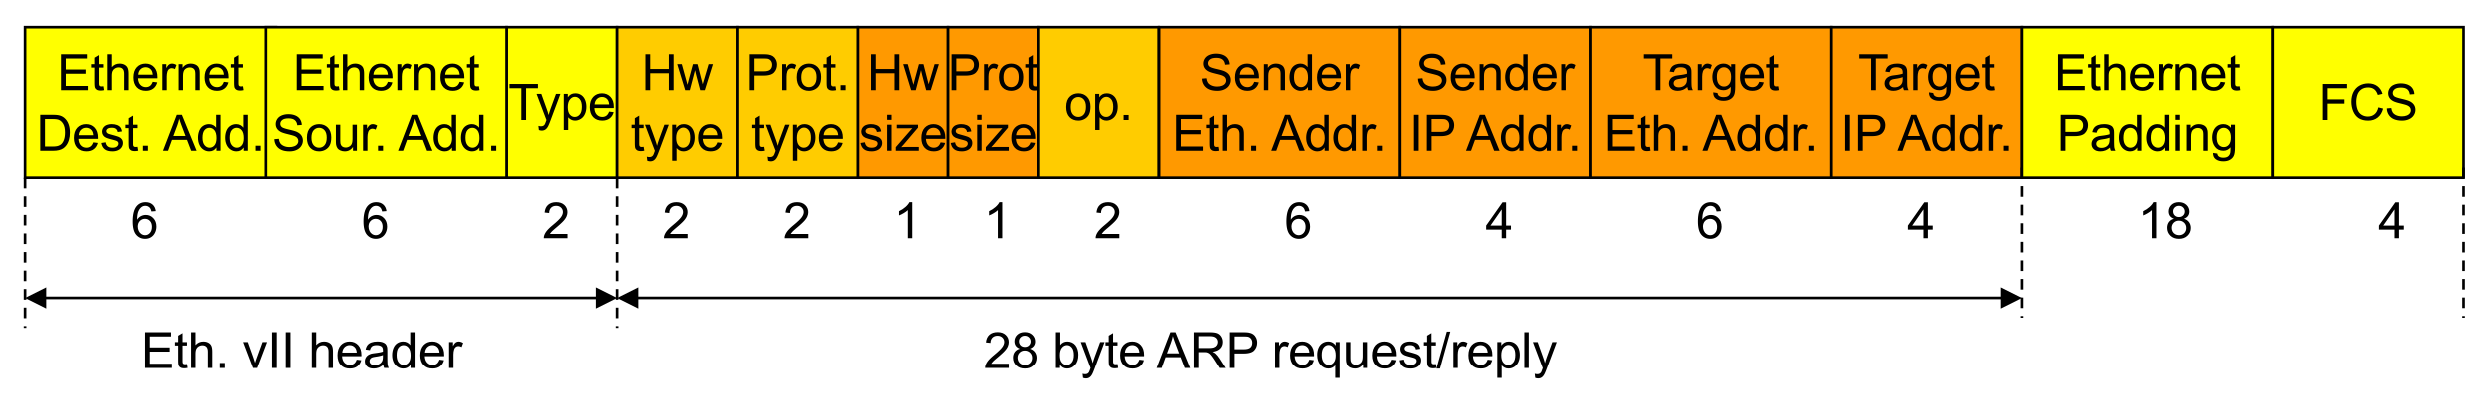
\includegraphics[width=1\textwidth]{images/frameethernet.png}
    \caption{Struttura di un frame Ethernet}
    \label{fig:frameethernet}
\end{figure}

Questo è il frame ethernet: 
in giallo ho l'header e la coda di ethernet , la coda svolge il ruolo di verificare che ci siano errori(fcs da 4 byte), il campo padding in coda serve a raggiungere i 64 byte(è un filler) minimi del frame totale tra ethernet e arp(arp è interno a l frame ethernet)
il frame deve avere una dimensione minima di 64 byte, il protocollo arp è quello arancione chiaro e scuro al centro.

Struttura del frame ethernet:
\begin{multicols}{2}
\begin{itemize}
    \item ethernet destination address: ind liv 2 del mittente - uguale a sender eth address
    \item ethernet source address
    \item type: tipologia tecnologia del livello 2
    \item hw type: specifica l'hardware che si sta usando al livello 2
    \item protocol type: specifica che procollo si vuole convertire dal liv 3 al 2(quindi non ha utilizzo esclusivo per indirizzi ip)
    \item hw size: dimensione indirizzo di liv 3
    \item prot size: dimensione indirizzo liv 2
    \item options:
    \item sender ethernet address: indirizzo liv 2 del mittente
    \item sender ip address: indirizzo liv 3 del mittente
    \item target ethernet address: indirizzo liv 2 del destinatario
    \item target ip address: indirizzo liv 3 del destinatario
    \item op: operazione che si vuole effettuare, 1 per richiesta arp, 2 per risposta arp
\end{itemize}
\end{multicols}

\subsubsection{Esempio ARP all'interno di una rete}

\begin{figure}[h!]
    \centering
    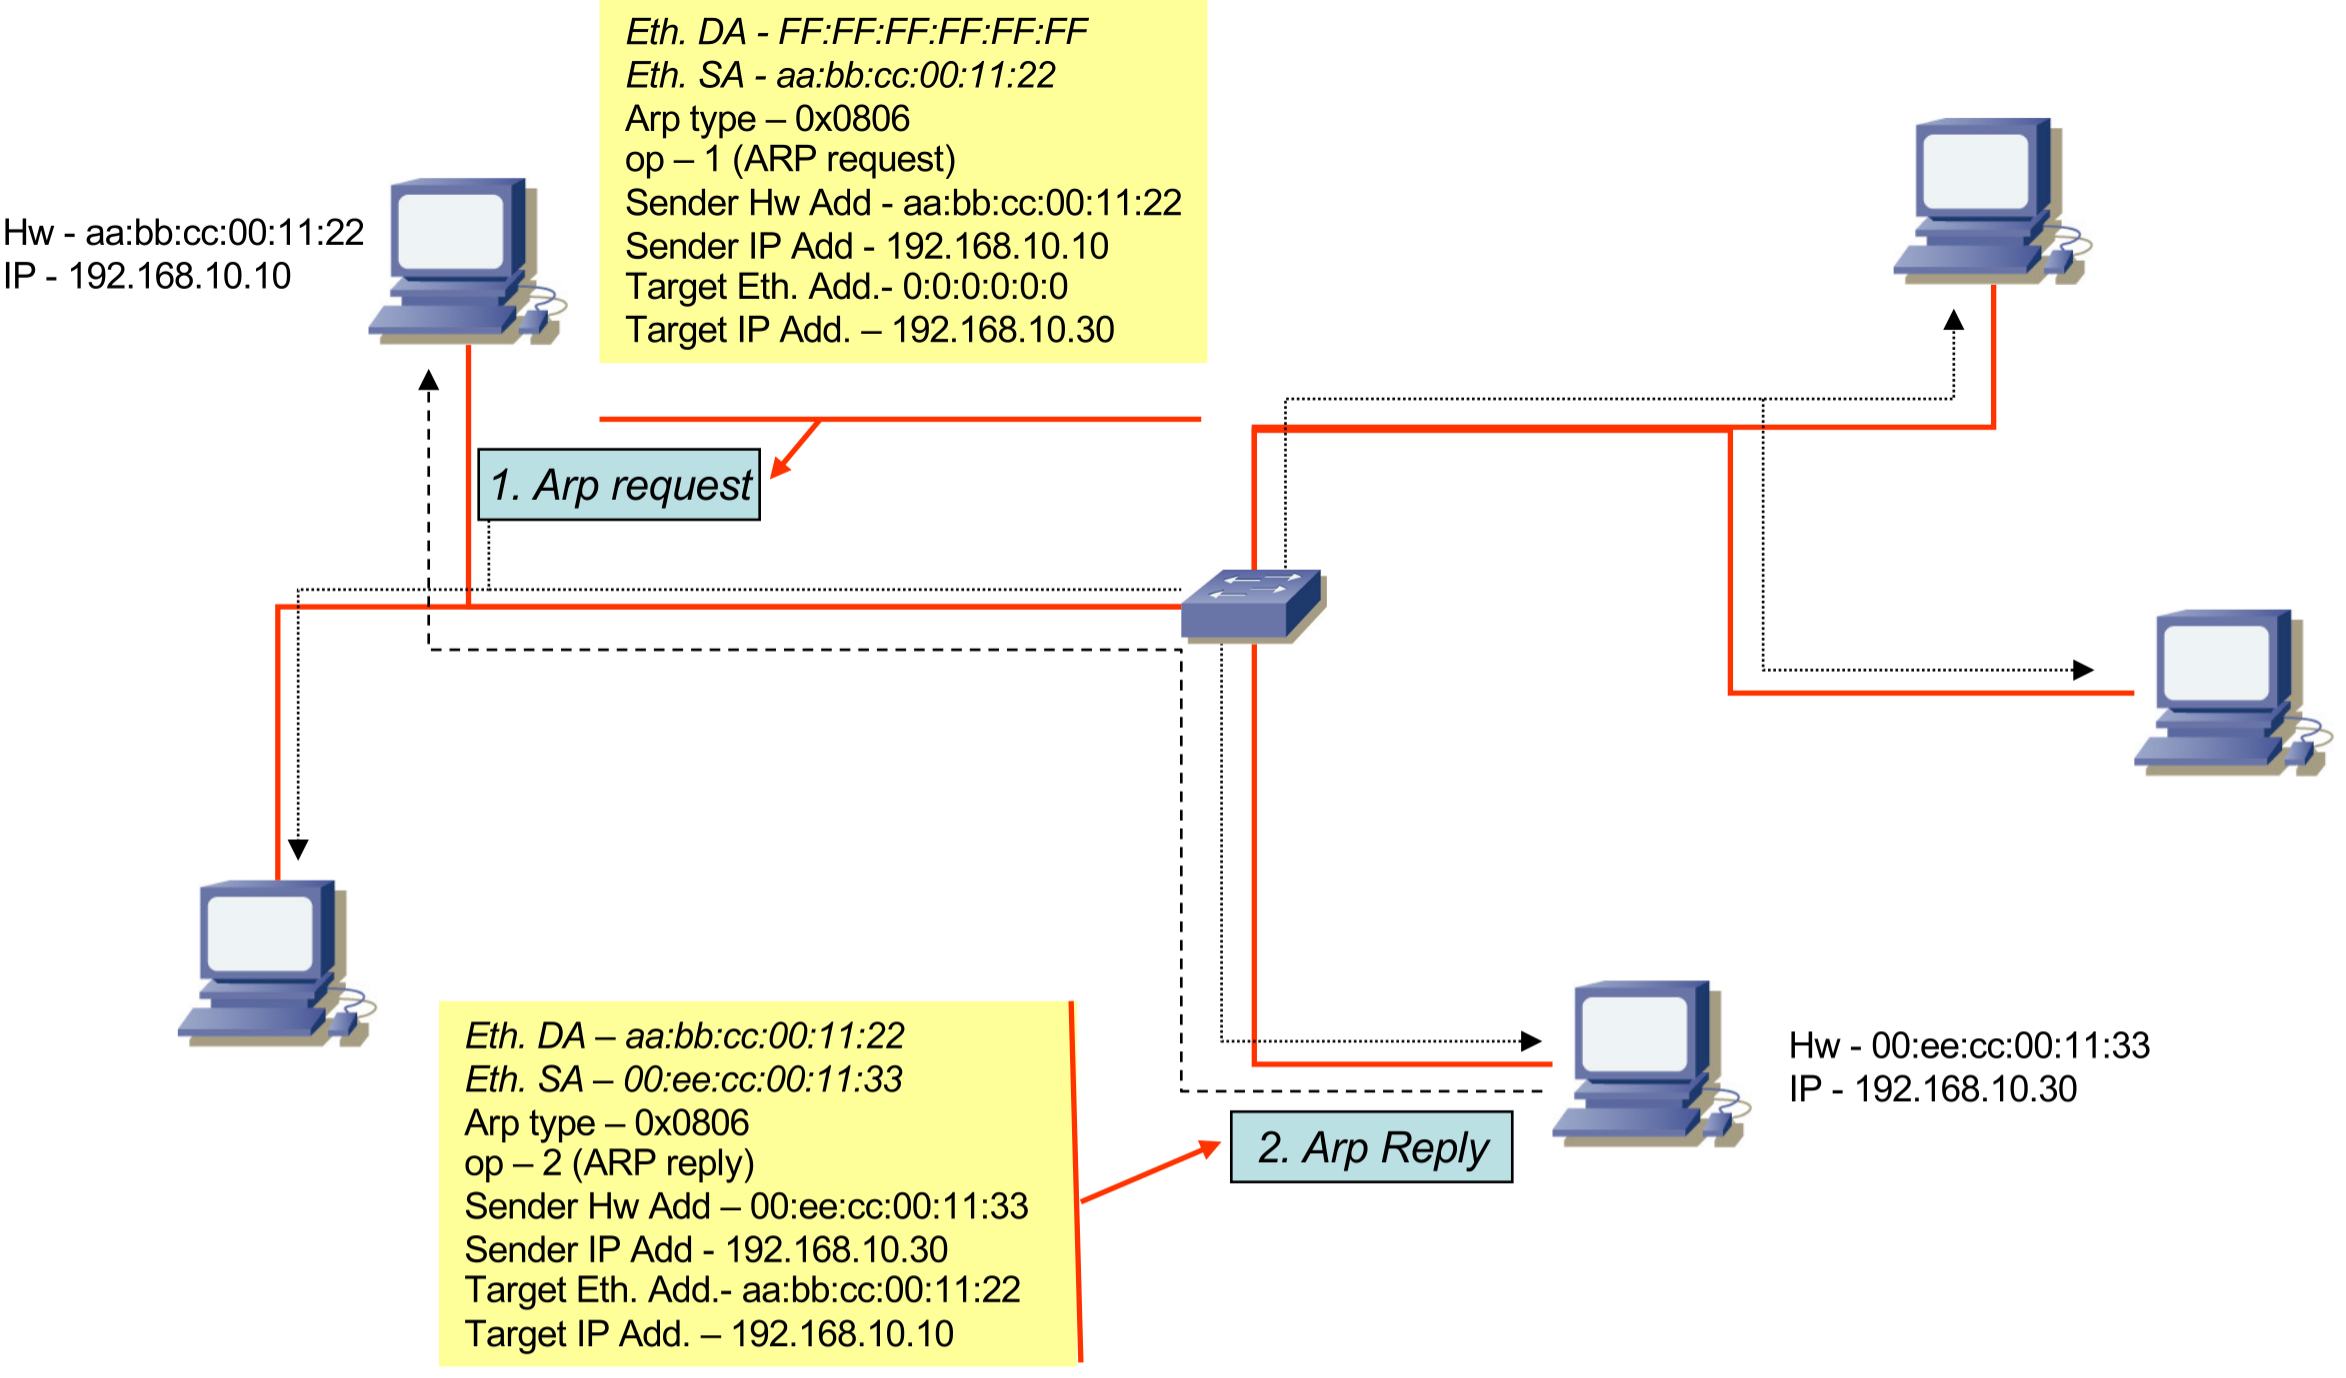
\includegraphics[width=1\textwidth]{images/esempioarp.png}
    \caption{Esempio di funzionamento del protocollo ARP}
    \label{fig:esempioARP}
\end{figure}

L'indirizzo hw è l'indirizzo fisico anche detto mac, è tipicamente in esadecimali ed è di 6 byte.

I riquadri in giallo sono pacchetti ARP utili alla comunicazione tra i due pc(visto che il dispositivo sta utilizzando arp per inviare un pacchetto allora sta usando un arp request, che viene segnato come op - 1 nel frame ethernet); i pacchetti in giallo quindi incapsulano una serie di informazioni del frame ethernet. 

Inoltre l'Ethernet destination address viene impostato a ff:ff:ff:ff:ff:ff (broadcast per indirizzi ARP) se viene effettuata un'ARP Request, questo perchè il mittente sta cercando di individuare l'indirizzo fisico del destinatario, di cui conosce solo l'ip, perciò utilzza ARP.

Nel momento della ARP request non so l'indirizzo ethernet del destinatario, ma so solo l'indirizzo ip, quindi ho tutti i byte del Ethernet address del target a 0.

Manderò quindi in broadcast(quindi multicast: a tutti i dispositivi della rete)(linee non tratteggiate) una richiesta a tutti i computer della rete, aspettando che il computer con l'indirizzo ip corrispondete a quello del target mi invii in unicast(linea tratteggiata) con un altro pacchetto ARP(arp reply, op - 2).

A questo punto il computer che ha inviato inizialmente l'ARP request riceve le info necessarie per poter inviare il pacchetto al destinatario. 
\newpage
\subsubsection{Esempio ARP in reti diverse}
IMPORTANTE: IL TCP(livello 4) si disinteressa di questo percorso, opera come se A e B fossero già collegati(end to end).

\begin{figure}[h!]
    \centering
    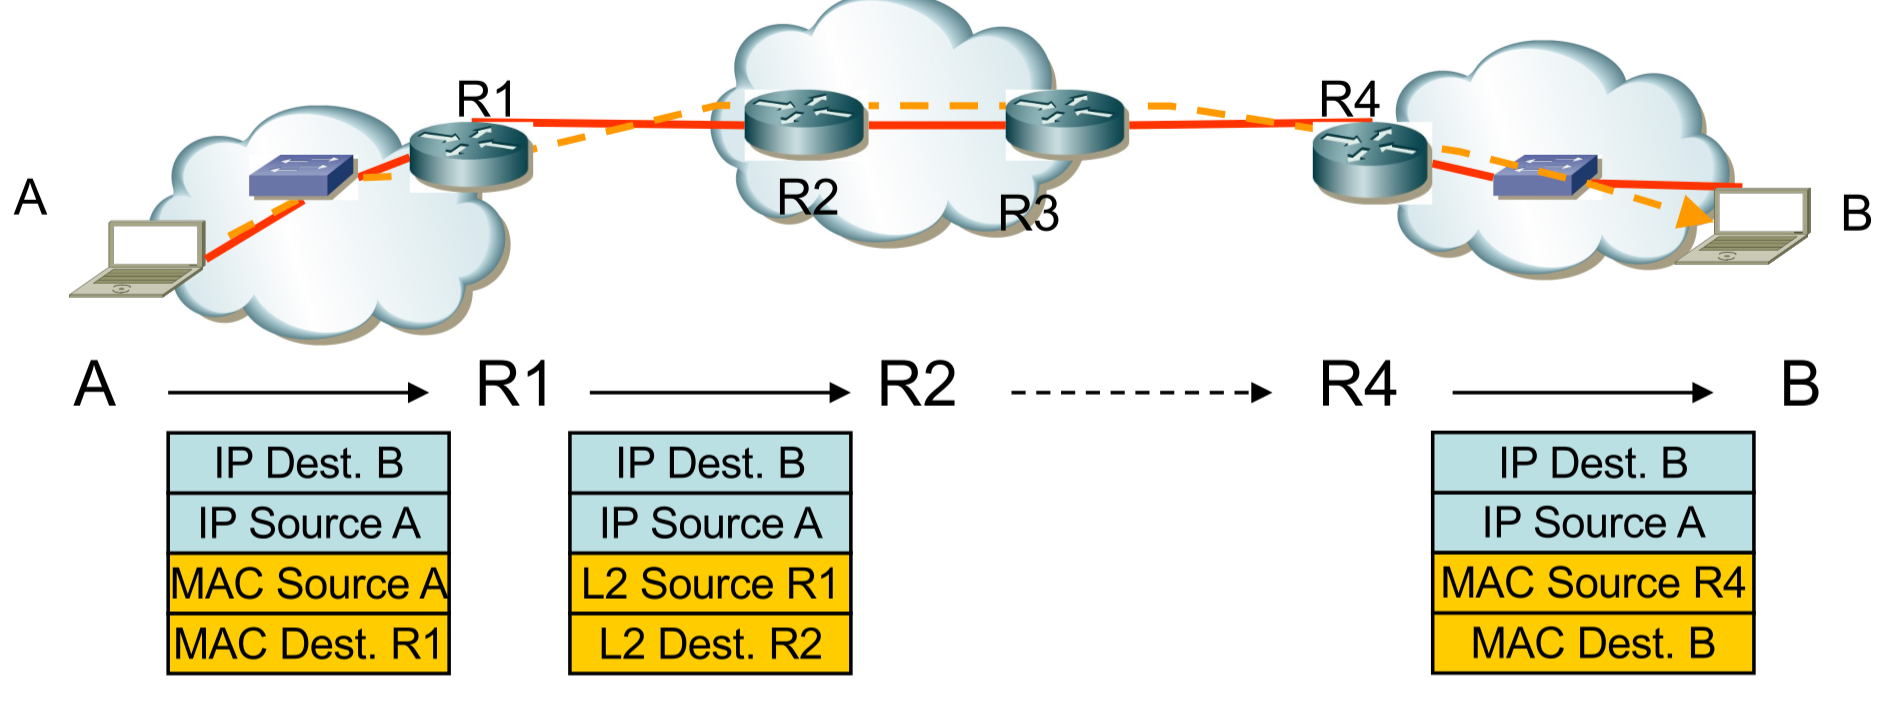
\includegraphics[width=1\textwidth]{images/esempioARPretidiverse.png}
    \caption{Esempio di funzionamento del protocollo ARP tra reti diverse}
    \label{fig:esempioARPretidiverse}
\end{figure}

\paragraph{Default gateway e tabelle di routing}

per scoprire se la rete del destinatario è la stessa da cui mando la richiesta arp: applico la mia maschera di rete all’ip del destinatario(la mia maschera di rete è un informazione che posseggo). quindi se la rete del destinatario non corrisponde a quella del mittente, per “uscire” e connettermi all’altra rete devo passare per il router. gli indirizzi di livello 3, quindi l’ip del destinatario e l’ip del mittente sono info che non variano tra un passaggio da un router all’altro, mentre quelli in giallo, gli indirizzi fisici(mac) variano tra router all’altro.
quindi il protocollo arp verrà applicato ad ogni passaggio tra un router all'altro cambiando quindi i mac source e mac destinatario, inserendo i mac dei dispositivi(router) tra cui avviene questo passaggio d’informazione. fino ad arrivare al dispositivo con l’indirizzo ip contenuto nel frame (ip dest B)
Il primo router a cui ci appoggiamo per l'inoltramento del pacchetto viene chiamato default gateway.

I router servono a connettere reti diverse, quindi se il destinatario non è nella mia rete allora mi appoggio al router, che ha un indirizzo ip di default, che è il default gateway.

Le tabelle di routing sono delle tabelle che i router utilizzano per sapere come inoltrare i pacchetti verso le reti di destinazione. Queste tabelle contengono informazioni sulle reti raggiungibili, i loro indirizzi IP e fisici.

A fine processo B legge i livelli 2 e 3 e riconosce i propri indirizzi MAC e IP, a quel punto può leggere il payload del pacchetto, che contiene i dati che A voleva inviare a B.

\paragraph{ARP nella stessa rete}
Se nel processo in cui cerco di capire se il destinatario sta nella mia rete o no scopro che sta nella mia rete allora non mi serve il router e posso inviare direttamente il pacchetto al destinatario, ma prima devo scoprire il suo indirizzo fisico(mac), quindi applico arp come fatto inizialmente.

\newpage
\subsection{Dynamic Host Configuration Protocol (DHCP) - configurazione automatica degli indirizzi IP tramite server DHCP}

 Un indirizzo ip può essere statico o dinamico, servers e router hanno tipicamente indirizzi statici.

Gli ind statici si configurano manualmente, quelli dinamici invece sono configurati tramite DHCP, un server che va configurato dall'utente ed è utile perchè fornisce: 
\begin{multicols}{3}
\begin{itemize}
    \item indirizzo ip del dispositivo
    \item netmask
    \item indirizzo ip del router
    \item indirizzo ip del server DNS
    \item lease time
\end{itemize}
\end{multicols}
Il lease time è il tempo in cui l'indirizzo ip è riservato al dispositivo, dopo di che il dispositivo deve richiedere un nuovo indirizzo ip;
è anche possibile ottenere un indirizzo IP riservato, sulla base dell'indirizzo fisico MAC.

\paragraph{DHCP relay - inoltro delle richieste DHCP}
Se nella rete locale non è disponibile un DHCP server, allora la richiesta può essere inoltrata  verso un'altra rete che dispone della funzione DHCP relay.

\paragraph{DHCP - funzionamento}
Questo protocollo fa uso dei UDP per la comunicazione tra client e server, e funziona in modo simile a ARP.

L'host che desidera un undirizzo IP si affida a questo protocollo per ottenerlo, inviando un messaggio DHCP discover, incapsulandolo in un pacchetto UDP, che viene inviato in broadcast a tutti i dispositivi della rete locale.

All'interno del pacchetto UDP, il mittente inserisce i seguenti indirizzi IP:
\begin{itemize}
    \item IP source address: l'indirizzo IP del mittente, che non è ancora stato assegnato, viene impostato momentaneamente a 0.0.0.0
    \item IP destination address: l'indirizzo IP del server DHCP, viene impostato a 255.255.255.255
\end{itemize}

Tutti gli eventuali server DHCP presenti nella rete rispondono in broadcast con un messaggio DHCP offer, che contiene le informazioni richieste dal client, come l'indirizzo IP assegnato, la netmask ecc\dots

Il client riceve le offerte dai server DHCP e sceglie una di esse, inviando un messaggio DHCP request al server scelto.

Infine il server DHCP conferma l'assegnazione dell'indirizzo IP con un messaggio DHCP ack.

    \begin{figure}[h!]
    \centering
    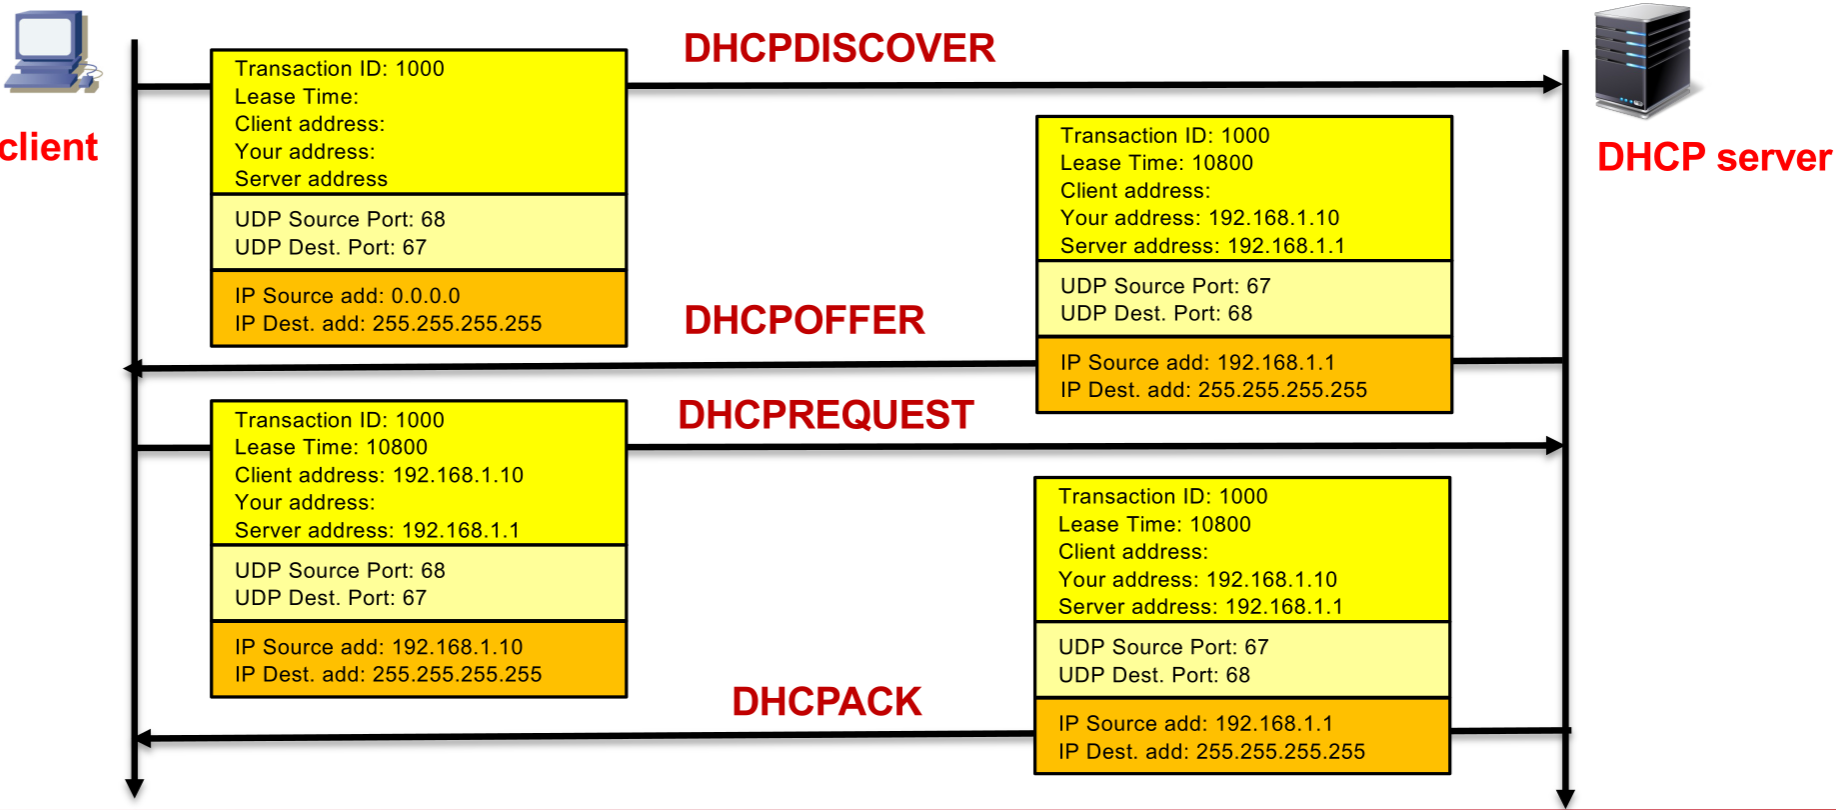
\includegraphics[width=1\textwidth]{images/dhcp.png}
    \caption{Funzionamento del protocollo DHCP}
    \label{fig:dhcp}
\end{figure}

\subsection{Zero-configuration networking}

Il zero-configuration networking è la configurazione della rete in assenza di server e amministratori, è ideale solo per reti piccole e semplici. Non è quindi un protocollo alternativo a DHCP.

\paragraph{Link-Local Address}
La IANA ha riservato a questo scopo un Link-Local Address: 169:254.0.0/16 

Gli indirizzi IP dei dispositivi nella rete vengono assegnati automaticamente, all'interno di un range specifico: [169.254.1.1 - 169.254.254]

\paragraph{ARP probe}
Quando un dispositivo si connette alla rete, invia un ARP probe per verificare se l'indirizzo IP scelto è già in uso. Se non riceve risposta, assume che l'indirizzo sia disponibile e lo utilizza. 
Se un altro host ha lo stesso indirizzo, sceglie casualmente un altro indirizzo IP all'interno dello stesso range.

\paragraph{ARP announcement}
Dopo aver scelto un indirizzo IP, il dispositivo invia un ARP announcement per informare gli altri dispositivi della rete del suo nuovo indirizzo. 

Questi indirizzi sono di tipo riservato e non possono essere usati per comunicare fuori dalla rete locale.



\subsection{Network Address Translation (NAT) - da IP privato a IP pubblico}


Il NAT è un software eseguito dal router di frontiera(ha il compito di far uscire dalla rete locale i pacchetti destinati ad indirizzi ip di altre reti).

Quindi è quel servizio che converte l'indirizzo privato del router di frontiera, in uno pubblico, cosè da comunicare con “l'esterno”. 
Perciò i router di frontiera delle altre reti non vedono l'indirizzo privato ma quello pubblico, convertito grazie al NAT.

Più precisamente, il NAT è una famiglia di tecniche/protocolli.

\paragraph{Funzionamento del NAT e tabelle di traduzione}

Tutti i datagram IP che viaggiano da (verso) la LAN hanno il medesimo indirizzo IP
mittente (destinazione), poichè il router di frontiera ha un solo indirizzo IP pubblico, che viene utilizzato per tutte le comunicazioni in uscita (entrata) dalla rete locale(LAN).

Il NAT utilizza una tabella di traduzione per mappare gli indirizzi IP privati della rete locale con l'indirizzo IP pubblico del router di frontiera; utilizzando le porte come ulteriore identificativi.

\begin{figure}[h!]
    \centering
    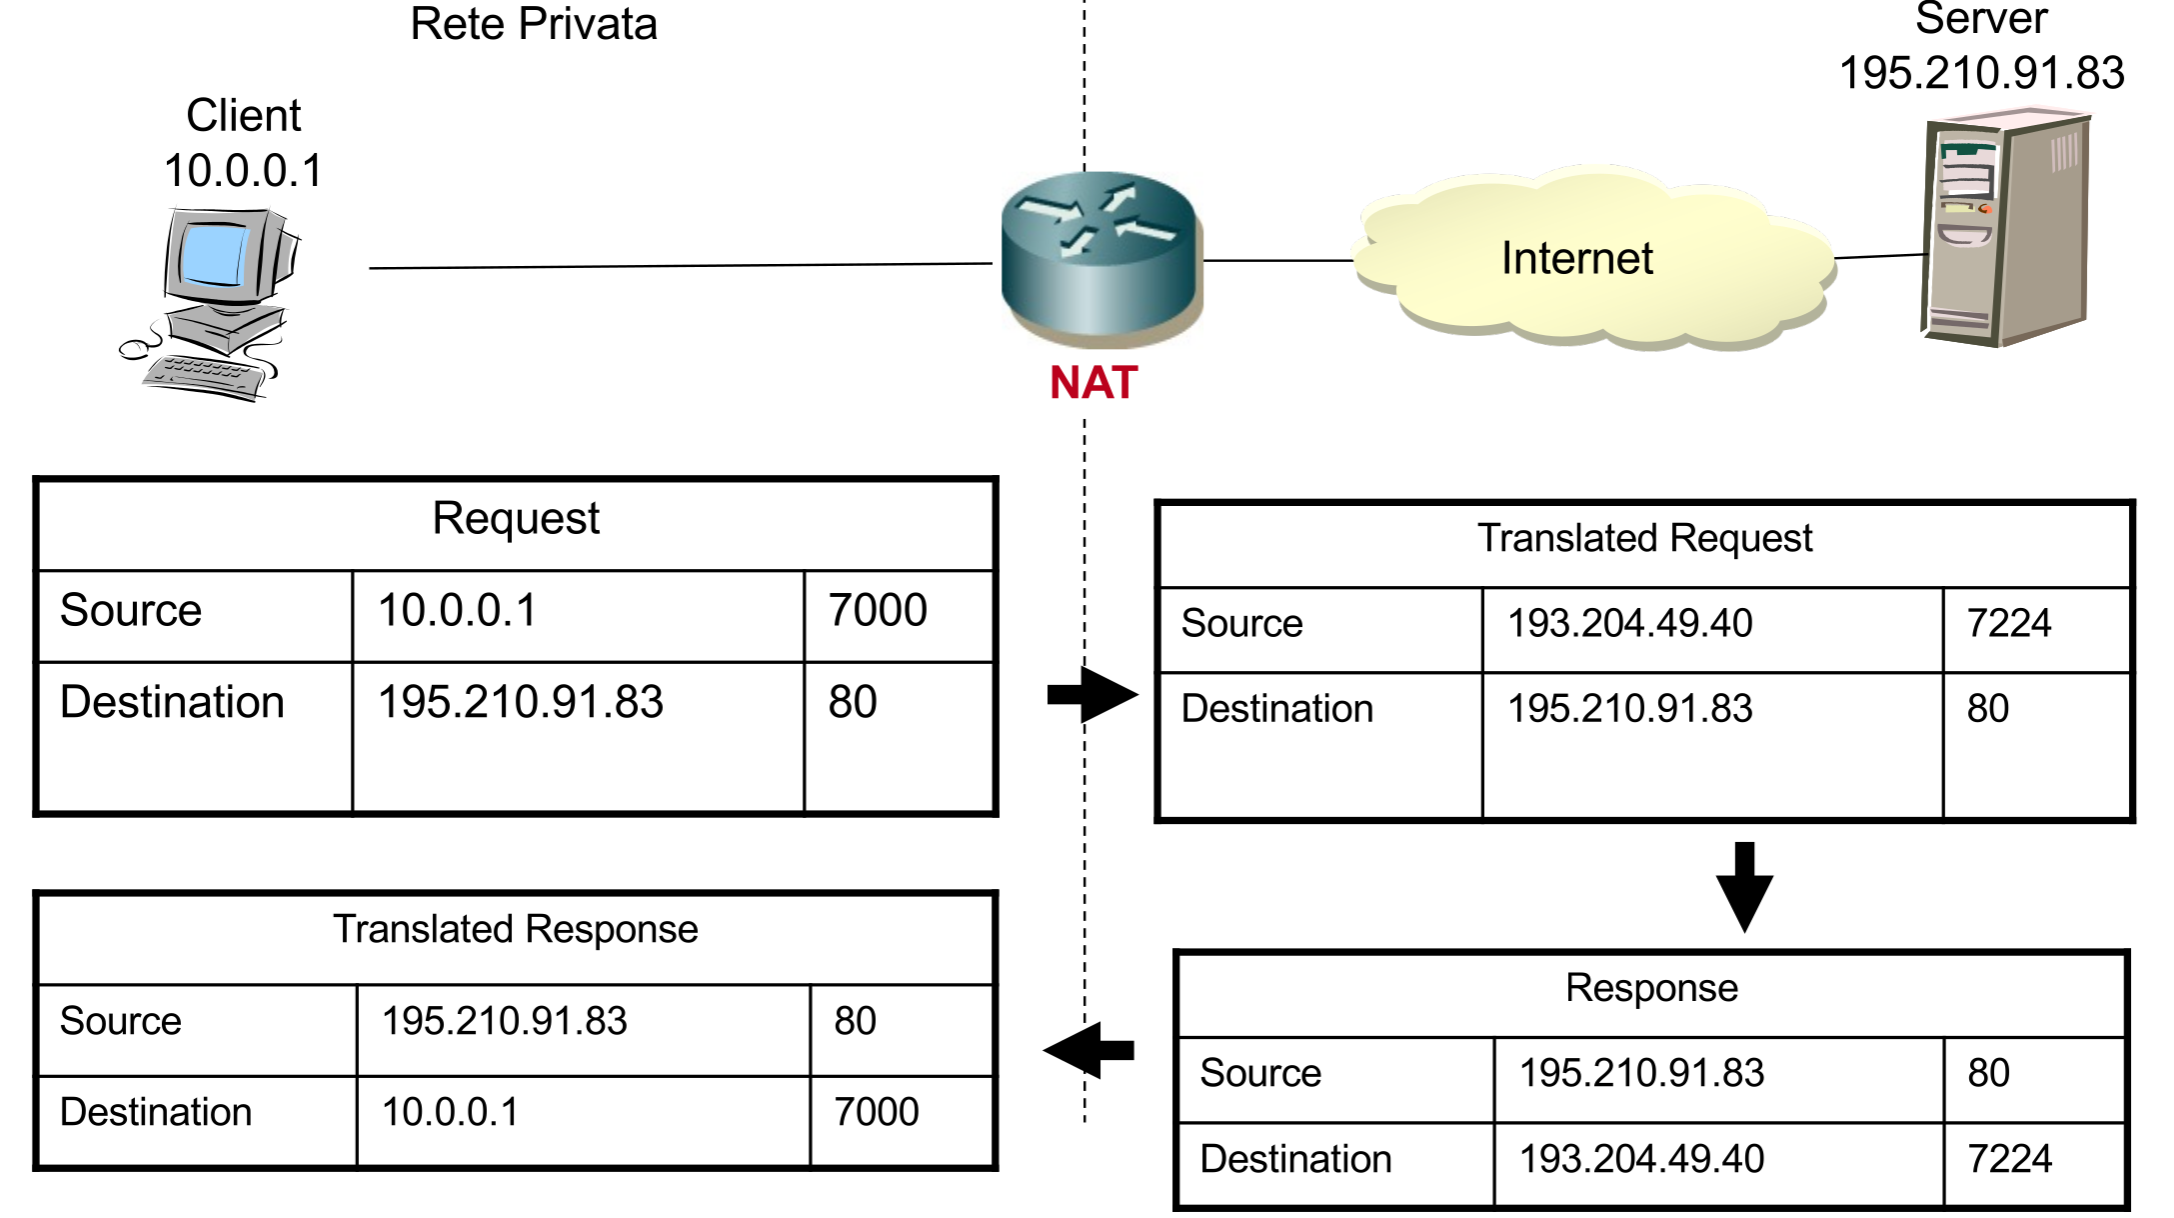
\includegraphics[width=0.85\textwidth]{images/nat.png}
    \caption{Funzionamento del NAT: traduzione degli indirizzi IP privati in indirizzi IP pubblici}
    \label{fig:nat}
\end{figure}

\newpage

\subsection{Internet control message protocol (ICMP) - diagnostica della rete}
I messaggi ICMP si dividono messaggi di errore e messaggi di richiesta; vengono inviati attraverso i pacchetti IP(protocol type 1);
questo protocollo serve a segnalare informazioni di controllo relative al livello di rete, un messaggio ICMP è composto dai campi type e code:
\begin{multicols}{2}
\begin{itemize}
    \item type: indica il tipo di messaggio ICMP
    \item code: dettagli sul tipo di messaggio
\end{itemize}
\end{multicols}


\begin{figure}[h!]
    \centering
    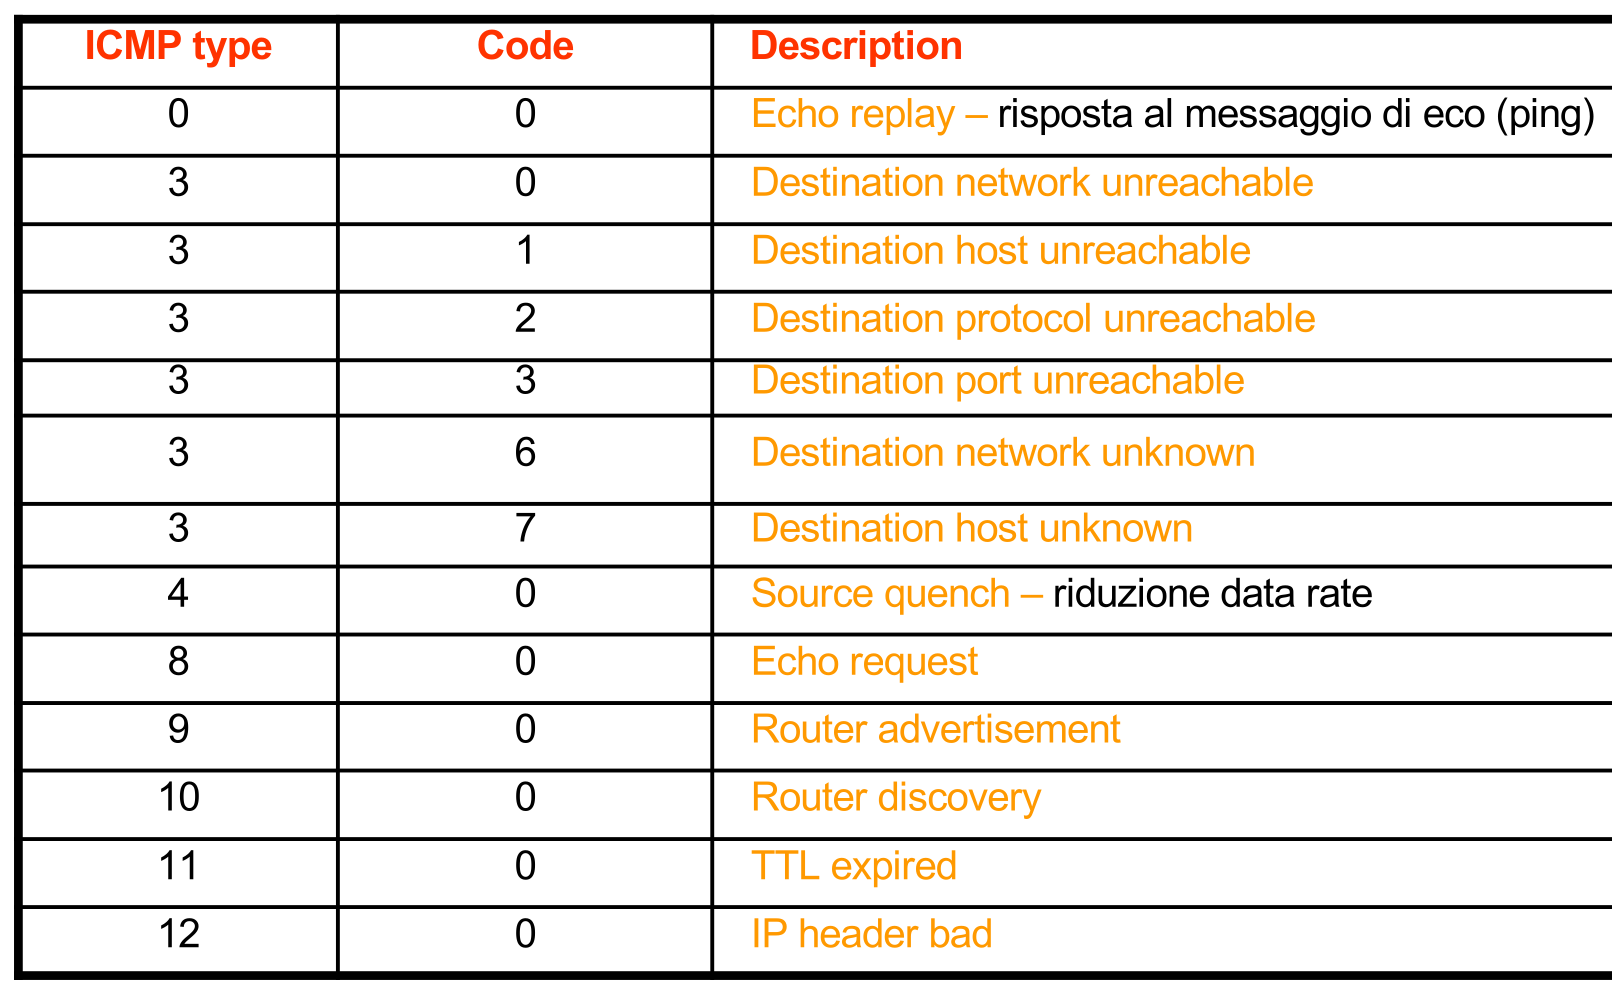
\includegraphics[width=0.67\textwidth]{images/comandiicmp.png}
    \caption{Principali comandi ICMP e loro utilizzo}
    \label{fig:comandiicmp}
\end{figure}



\paragraph{Esempio utilizzo di ICMP - ping}
Ad esempio, echo request e echo reply sono alla base del comando ping.
Type 8 corrisponde a echo request, mentre type 0 corrisponde a echo reply. 

\begin{figure}[h!]
    \centering
    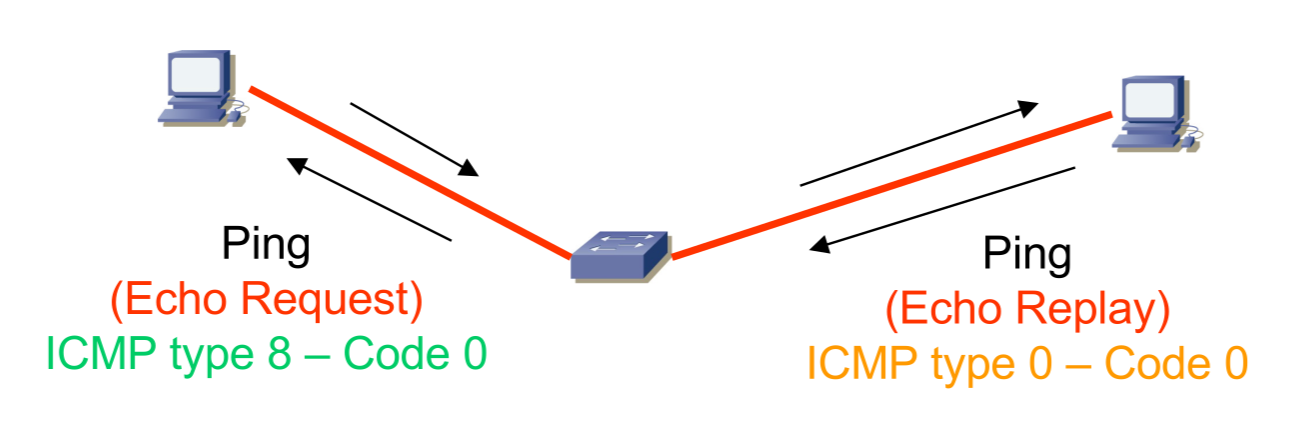
\includegraphics[width=0.55\textwidth]{images/pingicmp.png}
    \caption{Esempio di funzionamento di ICMP tramite il comando ping}
    \label{fig:pingicmp}
\end{figure}
\paragraph{Esempio utilizzo di ICMP - traceroute}
Tramite il traceroute( utilizzo dei ICMP type 11) scopro il percorso che sta seguendo il pacchetto 
comandi: traceroute sitoweb

\begin{figure}[h!]
    \centering
    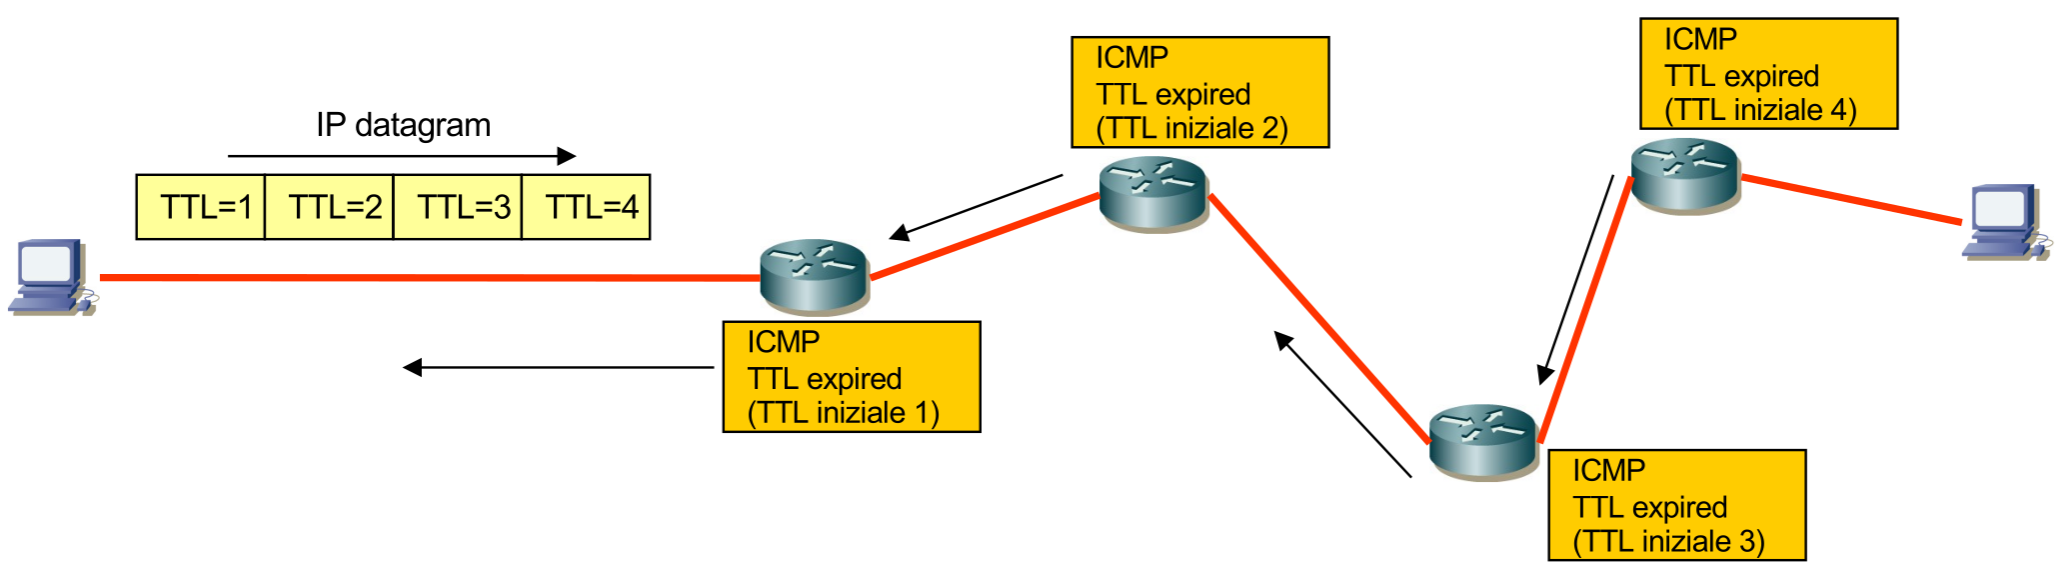
\includegraphics[width=0.8\textwidth]{images/traceroute.png}
    \caption{Esempio di funzionamento di ICMP tramite il comando traceroute}
    \label{fig:traceroute}
\end{figure}
\newpage




\section{Algoritmi di routing}
\subsection{Introduzione agli algoritmi di routing - tipologie}
Gli algoritmi di routing sono utilizzati dai router per determinare il percorso migliore che i pacchetti devono seguire per raggiungere la loro destinazione.

Questi algoritmi possono essere classificati in base al loro uso o meno delle tabelle di routing o se sono gerarchici.

\begin{figure}[h!]
    \centering
    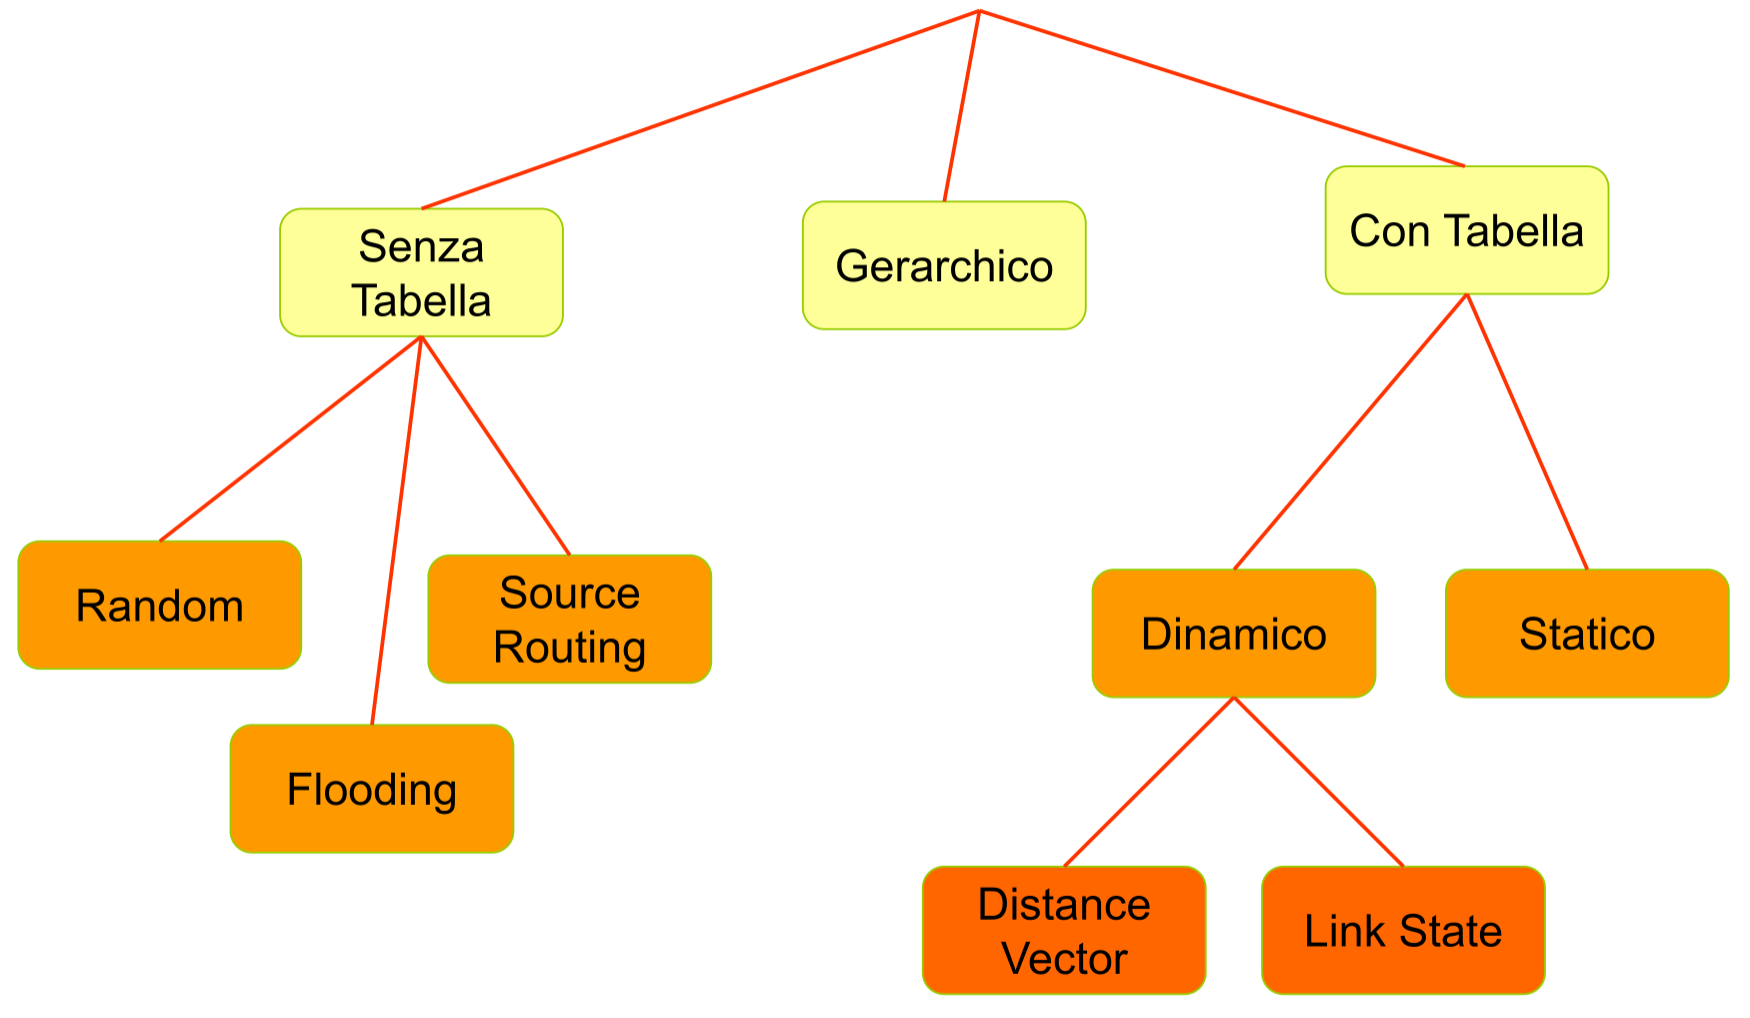
\includegraphics[width=1\textwidth]{images/routingtipologie.png}
    \caption{Tipologie di algoritmi di routing}
    \label{fig:routingtipologie}
\end{figure}

\begin{itemize}
    \item Con tabella:  il router conserva in memoria una tabella per capire qual è la strada migliore, contiene dati per scegliere la strada migliore
    \begin{figure}[h!]
        \centering
        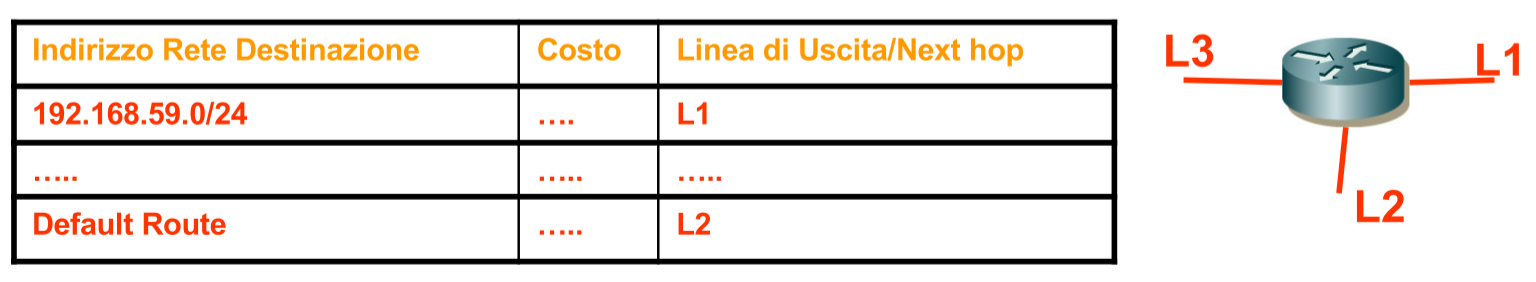
\includegraphics[width=1\textwidth]{images/tabellarouting.png}
        \caption{Esempio di tabella di routing}
        \label{fig:tabellarouting}
    \end{figure}
    Come costo si intende il numero di hop, la banda, l'affidabilità, il ritardo o anche un valore inserito manualmente; dipende strettamente dal metodo che si vuole utilizzare.

    \item Senza tabella: includono il routing random, il flooding e il source routing
    
    \item Gerarchici: i router affidano le scelte di routing ad altri router "più intelligenti"?
\end{itemize}

!Instradare significa scegliere il percorso migliore per raggiungere la destinazione, il forewarding invece è l'azione di inviare il pacchetto per la strada scelta!

\subsection{Metriche per il costo del percorso}
Il costo del percorso viene calcolato sulla base di diverse metriche:
\begin{itemize}
    \item \textbf{\textit{Bandwidth}}: la capacità di un link (es. generalmente un link a 10 Mbps è preferibile rispetto ad una linea a 64 kbps)
    \item \textbf{\textit{Delay}}: il tempo necessario ad ogni pacchetto per andare dalla sorgente alla destinazione
    \item \textbf{\textit{Load}}: il carico di lavoro degli elementi della rete come i router o i link
    \item \textbf{\textit{Reliability}}: l'affidabilità, generalmente riferita al tasso di errore di ogni singolo link
    \item \textbf{\textit{Hop count}}: il numero di router che un pacchetto deve attraversare per raggiungere la destinazione
    \item \textbf{\textit{Ticks}}: il ritardo di un collegamento dati in multipli di un \textit{IBM PC clock tick} (circa 55 ms)
    \item \textbf{\textit{Cost}}: un valore arbitrario, generalmente basato sulla banda, sul costo economico di un link, o su altre misure stabilite dall'amministratore di rete
\end{itemize}

\paragraph{Cosa fa il router?}

Il router è un dispositivo fondamentale nelle reti di comunicazione, in quanto si occupa di instradare i pacchetti dati tra reti diverse. Il suo compito principale è ricevere i pacchetti in ingresso su una delle sue interfacce, esaminare l'indirizzo IP di destinazione e, in base alle informazioni contenute nella propria tabella di routing, decidere su quale interfaccia inoltrare ciascun pacchetto affinché raggiunga la destinazione finale nel modo più efficiente possibile. Il router aggiorna periodicamente la propria tabella di routing tramite protocolli specifici e può adattare le proprie decisioni in base ai cambiamenti della topologia di rete. In sintesi, il router permette la comunicazione tra reti diverse, ottimizzando il percorso dei dati e garantendo che i pacchetti raggiungano correttamente il destinatario.

\paragraph{Funzionamento della tabella di routing}

Quando un router riceve un datagramma, esegue i seguenti passaggi per determinare dove inoltrarlo:
\begin{enumerate}
    \item Cerca nella tabella di routing una entry con lo stesso indirizzo di rete del destinatario del datagramma ricevuto.
    \item Se la entry corrisponde a una rete direttamente connessa al router, viene individuata la sottorete e il datagramma è inoltrato direttamente.
    \item Se la entry corrisponde a una rete remota, il datagramma è inoltrato (forwarding) verso il prossimo hop specificato nella tabella.
    \item Se nessuna entry è trovata, viene utilizzato il \textit{default route}
\end{enumerate}

\newpage

\subsection{Instradamento gerarchico - protocolli intra e inter AS}
Al fine di comprendere il routing è indispensabile introdurre il concetto di Autonomous System(AS).

Un AS è l'insieme di router amministrati dallo stesso gestore; è possibile distinguere i vari protocolli di routing proprio sulla base di questo.

Infatti i protocolli che lavorano all'interno di un AS vengono chiamati intra AS, mentre quelli che operano tra Autonomous Systems differenti vengono detti inter AS.

\begin{figure}[h!]
    \centering
    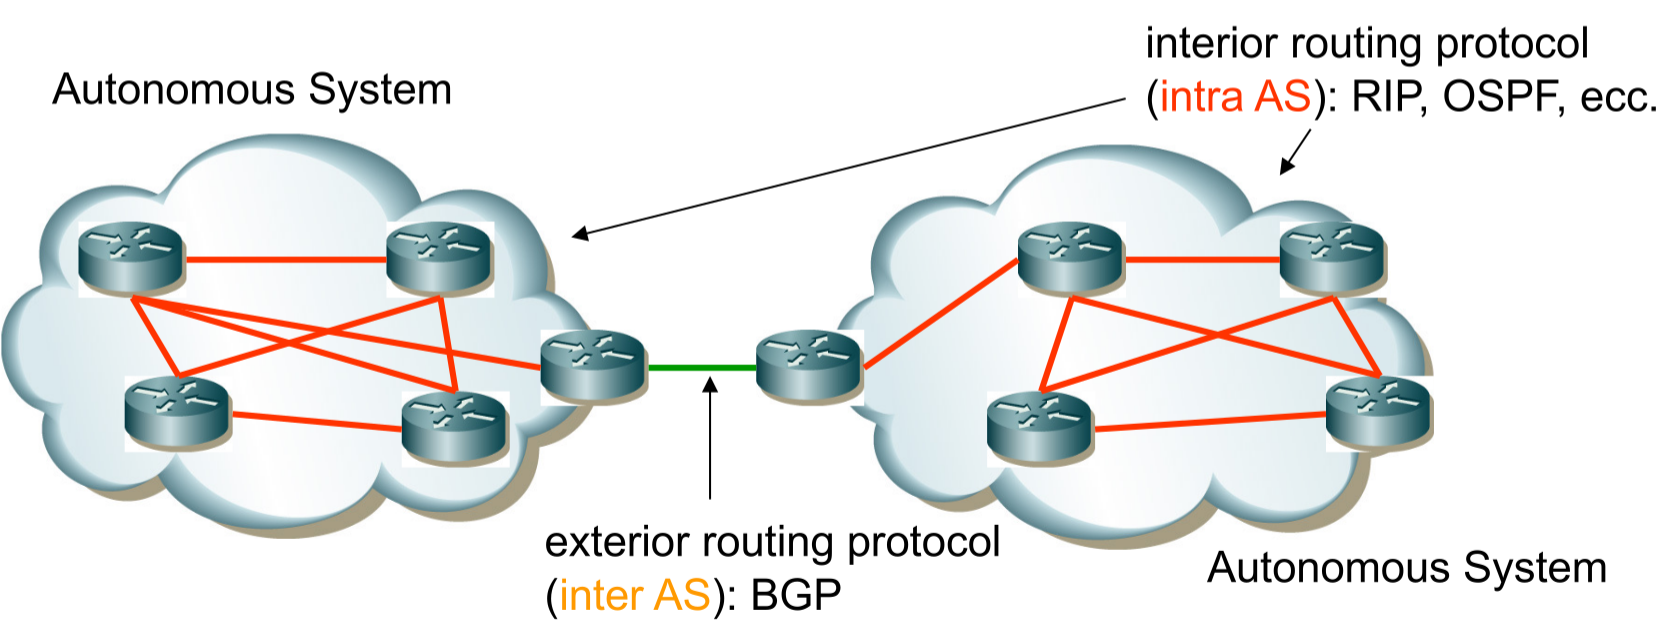
\includegraphics[width=0.8\textwidth]{images/asgerarchia.png}
    \caption{Esempio di gerarchia tra Autonomous Systems (AS)}
    \label{fig:asgerarchia}
\end{figure}



\subsection{Distance Vector}

È una famiglia di algoritmi di routing in cui ogni router scambia informazioni con i vicini, usa l'algoritmo di Bellman-Ford per calcolare il percorso più breve.
Un algoritmo di routing che fa uso di tabelle dinamiche è il distance vector:

ogni rouoter prende decisioni in modo autonomo; ogni router invia in modo periodico ai router vicini i “vettori delle distanze”(distance vector).

Le colonne della tabella che interessano particolarmente questo algoritmo sono quella dei costi e quella delle destinazioni note. 

In questo modo tra i router ci si scambiano informazioni utili al routing stesso, prendendo informazioni dai router vicini

Il vettore distanza quindi comunica ai vicini i percorsi che conosce e il costo di tali percorsi(percorsi che passano dal router che condivide tali percorsi)
le tabelle sono dinamiche perchè la topologia della rete può cambiare nel tempo.

\begin{figure}[h!]
    \centering
    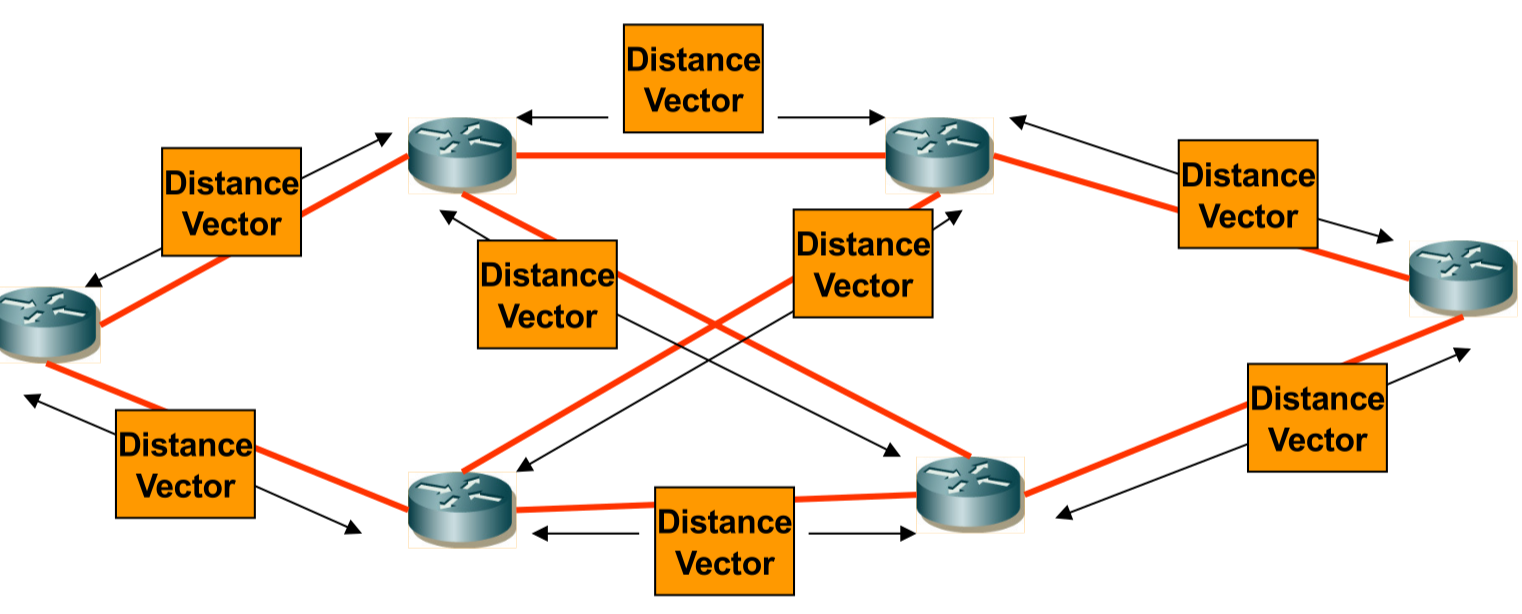
\includegraphics[width=0.9\textwidth]{images/distancevector.png}
    \caption{Esempio di funzionamento dell'algoritmo Distance Vector}
    \label{fig:distancevector}
\end{figure}
\newpage
\subsection{Algoritmo Bellman-Ford}
Il funzionamento dell'algoritmo di routing distance-vector porta ad una
soluzione che si otterrebbe equivalentemente applicando l'algoritmo di
Bellman-Ford per la ricerca del cammino a costo minimo in un grafo.

I router non applicano questo algoritmo, ma la
soluzione finale cui si giunge è identica.

Questo algorimo lavora su una rappresentazione globale del grafo, cosa che nei ruouter reali non accade poichè non conoscono tutta la rete, ma solo le info sui e dei vicini diretti.

!I protocolli distance vector sono una versione distribuita del Bellman-Ford, cioè: l'algoritmo non è eseguito da un singolo punto centrale, ma ogni nodo della rete (es. ogni router) esegue una parte dell'algoritmo.!


\paragraph{Variabili}
\begin{multicols}{2}
\begin{itemize}
    \item $s$ è il router da cui parte l'algoritmo e di cui ci interessa calcolare il costo minimo
    \item $h$ indica il numero dei salti
    \item $j$ indica un nodo
    \item $i$ indica un nodo differente da $j$
    \item $D_j^{(h)}$ è il costo del cammino minimo tra la sorgente $s$ e il nodo $j$ con massimo $h$ salti
    \item $d_{ij}$ è il costo del collegamento diretto tra i nodi $i$ e $j$; questo costo è infinito se i nodi non sono collegati direttamente
\end{itemize}
\end{multicols}



\paragraph{Fasi dell'algoritmo}
\begin{enumerate}
    \item Inizializzazione: $h = 0$
    \begin{itemize}
        \item La distaza del nodo da se stesso $D_s^{(0)} = 0$
        \item La distanza tra s e i nodi non diretti è infinita $D_j^{(0)} = \infty$ per tutti i $j \neq s$
    \end{itemize}
    \item Iterazione: per ogni $h > 0$

    Hop successivo $h = h + 1$ 

    Calcolo le dei cammini al salto successivo $D_j^{(h)} = \min_i [D_i^{(h-1)} + d_{ij}^{(h-1)}]$

     \item Verifica: tramite questo controllo capisco se il cammino $D_j^{(h)}$ calcolato è uguale al precedente, se così fosse allora non ha senso continuare e si setta come $h_{max}$ quello precedente, si ferma l'algoritmo; in caso contrario l'algortmo prosegue dal passaggio due. 
     
    If $D_j^{h} = D_j^{h-1} \quad \forall j \neq s$
    
    then $h_{max} = h - 1$; stop
    
    else go to 2
\end{enumerate}
\newpage
\paragraph{Esempio}

Il primo passo è calcolare i costi dei cammini quando h = 0, ricordando che quando non c'è collegamento diretto avrò costo infinito.

\begin{figure}[h!]
    \centering
    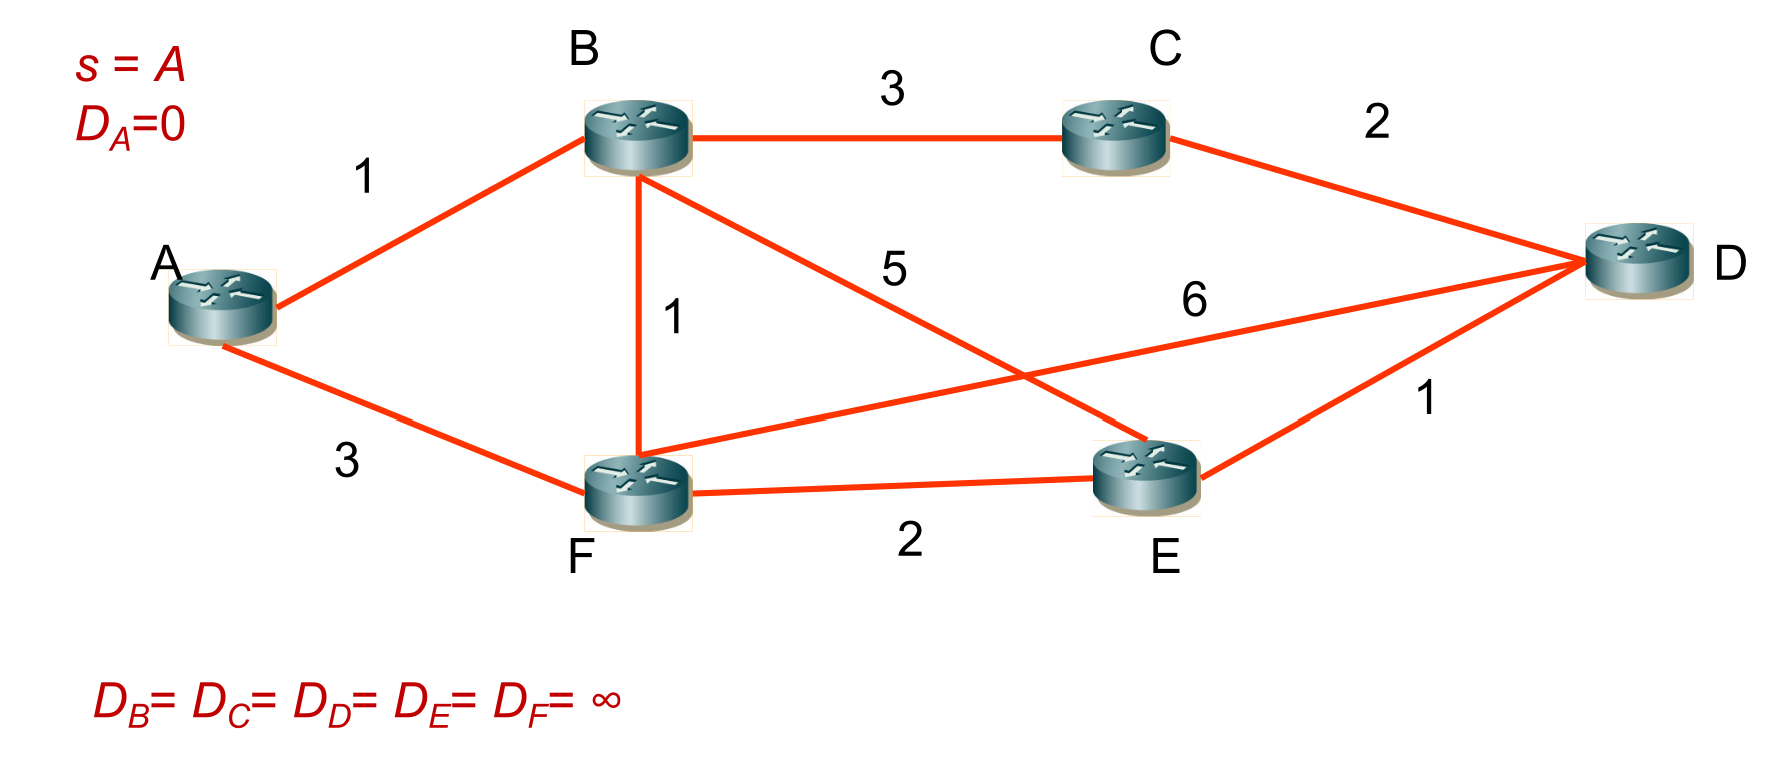
\includegraphics[width=0.75\textwidth]{images/bf1.png}
    \caption{Esempio di applicazione dell'algoritmo di Bellman-Ford - Passo 0}
    \label{fig:bf1}
\end{figure}

\vspace{1em}
\noindent\rule{\linewidth}{0.4pt}
\vspace{1em}

Poi si calcolano i costi dei cammini quando h = 1, quindi con al massimo un salto.

\begin{itemize}
    \item $D_B^{(1)} = \min [D_A^{(0)} + d_{AB}, D_C^{(0)} + d_{CB}, D_D^{(0)} + d_{DB}, D_E^{(0)} + d_{EB}, D_F^{(0)} + d_{FB}, D_B^{(0)}] = $
   
    $\min [0 + 1, \infty + 3, \infty + \infty, \infty + 5, \infty + 1, \infty] = 1$
    \item $D_C^{(1)} = \min [D_A^{(0)} + d_{AC}, D_B^{(0)} + d_{BC}, D_D^{(0)} + d_{DC}, D_E^{(0)} + d_{EC}, D_F^{(0)} + d_{FC}, D_C^{(0)}] = $
    
    $\min [0 + 3, \infty + 3, \infty + \infty, \infty + 2, \infty + \infty, \infty] = 3$
    \item $D_D^{(1)} = \min [D_A^{(0)} + d_{AD}, D_B^{(0)} + d_{BD}, D_C^{(0)} + d_{CD}, D_E^{(0)} + d_{ED}, D_F^{(0)} + d_{FD}, D_D^{(0)}] = $ 
    
    $\min [0 + \infty, \infty + \infty, \infty + \infty, \infty + 1, \infty + 5, \infty] = \infty$
    \item $D_E^{(1)} = \min [D_A^{(0)} + d_{AE}, D_B^{(0)} + d_{BE}, D_C^{(0)} + d_{CE}, D_D^{(0)} + d_{DE}, D_F^{(0)} + d_{FE}, D_E^{(0)}] = $ 
    
    $\min [0 + \infty, \infty + 5, \infty + 2, \infty + 1, \infty + \infty, \infty] = \infty$
    
    \item $D_F^{(1)} = \min [D_A^{(0)} + d_{AF}, D_B^{(0)} + d_{BF}, D_C^{(0)} + d_{CF}, D_D^{(0)} + d_{DF}, D_E^{(0)} + d_{EF}, D_F^{(0)}] = $ 
    
    $\min [0 + \infty, \infty + 1, \infty + \infty, \infty + 5, \infty + \infty, \infty] = \infty$
\end{itemize}

\begin{figure}[h!]
    \centering
    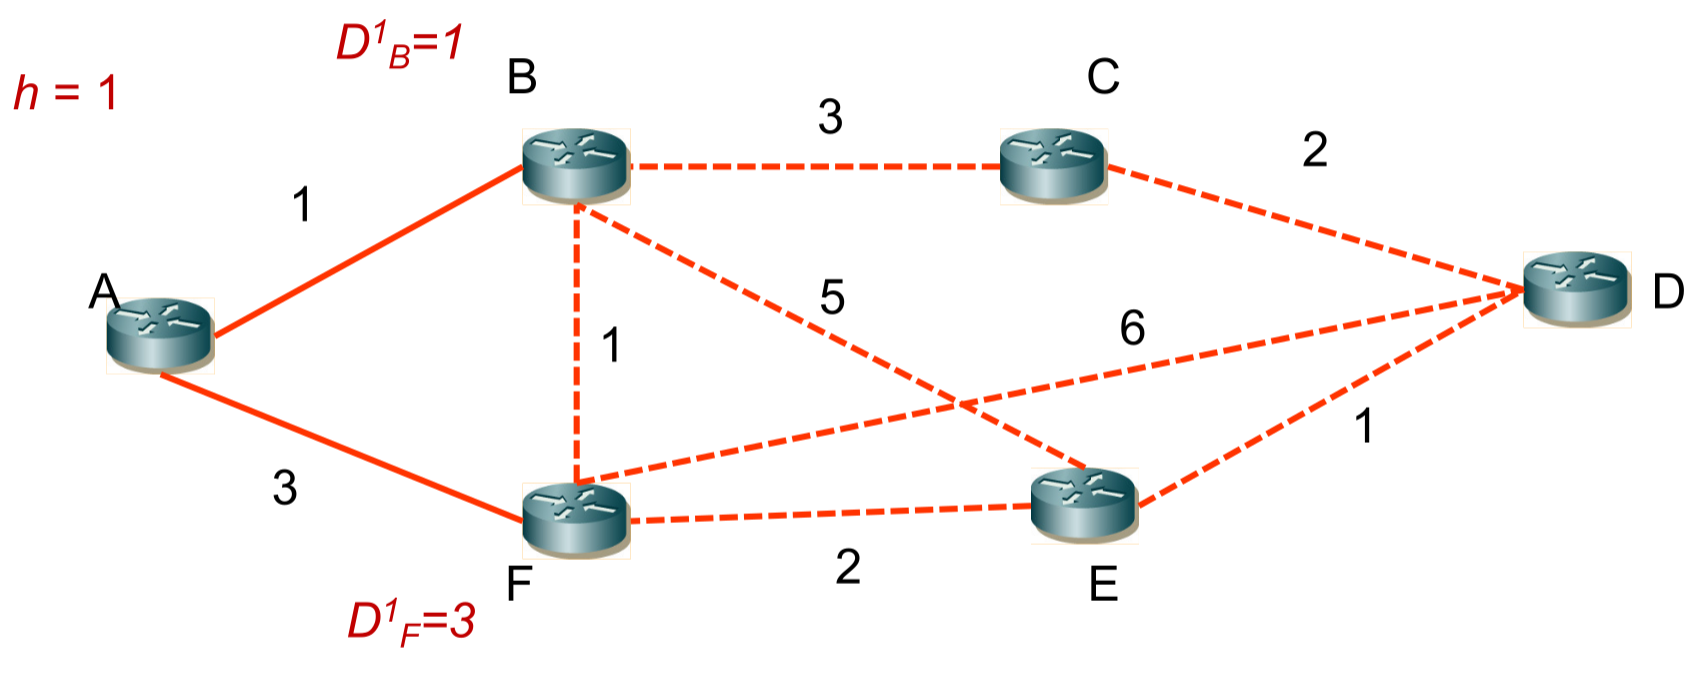
\includegraphics[width=0.75\textwidth]{images/bf2.png}
    \caption{Esempio di applicazione dell'algoritmo di Bellman-Ford - Passo 1}
    \label{fig:bf2}
\end{figure}

\newpage


\begin{itemize}
    \item $D_B^{(2)}$ = $\min [0 + 1, 3 + 3, \infty + \infty, \infty + 5, \infty + 1, 1] = 1$
    \item $D_C^{(2)}$ = $\min [0 + 3, 1 + 3, \infty + \infty, \infty + 2, \infty + \infty, 3] = 3$
    \item $D_D^{(2)}$ = $\min [0 + \infty, 1 + \infty, 3 + 6, \infty + 1, \infty + 5, \infty] = \infty$
    \item $D_E^{(2)}$ = $\min [0 + \infty, 1 + 5, 3 + 2, \infty + 1, \infty + \infty, \infty] = 5$
    \item $D_F^{(2)}$ = $\min [0 + \infty, 1 + 1, 3 + \infty, \infty + 5, \infty + \infty, \infty] = 2$
\end{itemize}

\begin{figure}[h!]
    \centering
    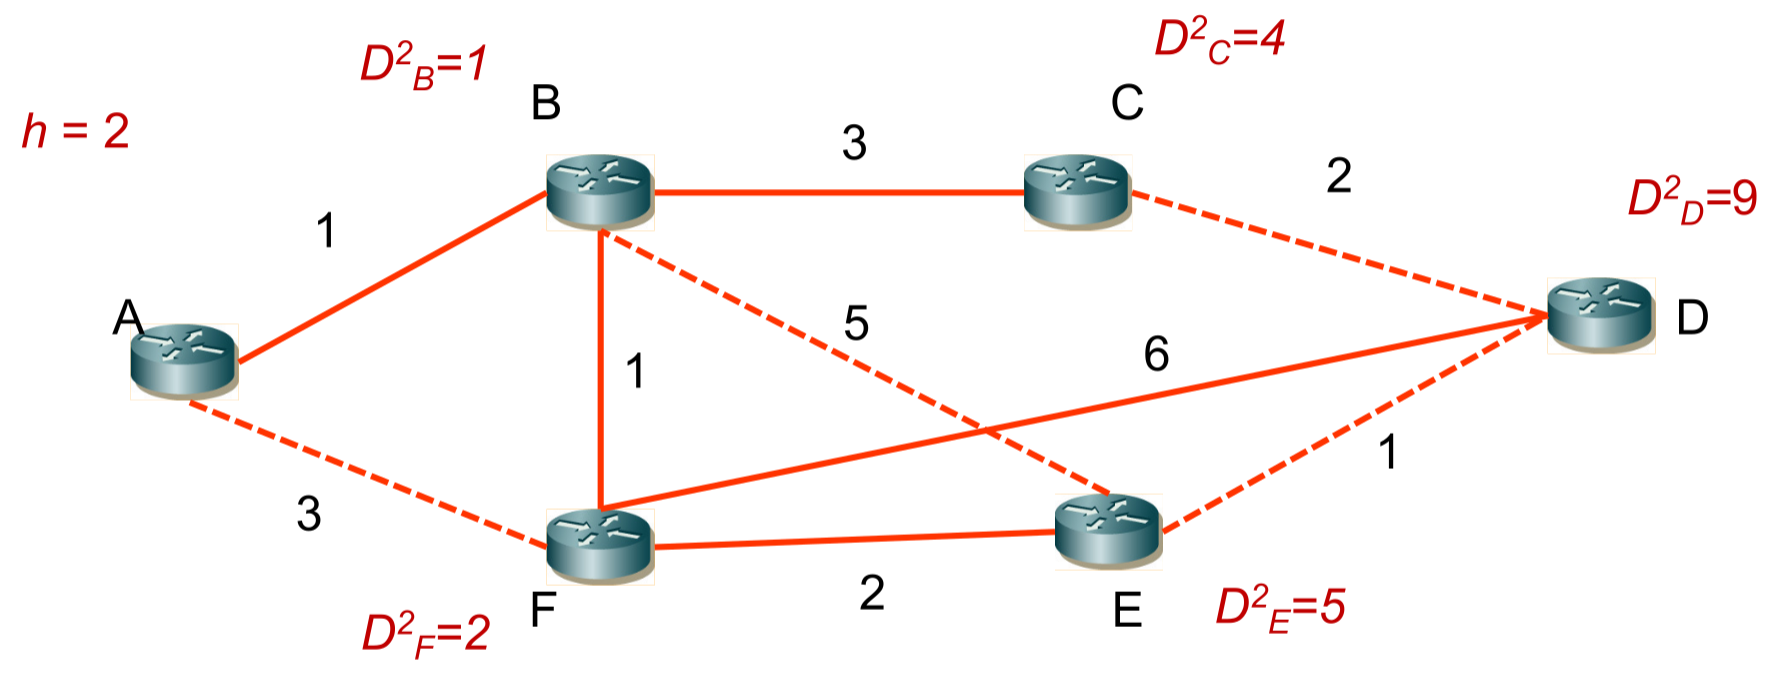
\includegraphics[width=0.85\textwidth]{images/bf3.png}
    \caption{Esempio di applicazione dell'algoritmo di Bellman-Ford - Passo 2}
    \label{fig:bf3}
\end{figure}

\vspace{1em}
\noindent\rule{\linewidth}{0.4pt}
\vspace{1em}


\begin{itemize}
    \item $D_B^{(3)}$ = $\min [0 + 1, 3 + 3, \infty + \infty, 5 + 5, 2 + 1, 1] = 1$
    \item $D_C^{(3)}$ = $\min [0 + 3, 1 + 3, \infty + \infty, 5 + 2, 2 + \infty, 3] = 3$
    \item $D_D^{(3)}$ = $\min [0 + \infty, 1 + \infty, 3 + \infty, 5 + 1, 2 + 5, \infty] = 6$
    \item $D_E^{(3)}$ = $\min [0 + \infty, 1 + 5, 3 + 2, \infty + 1, 2 + \infty, 5] = 5$    
    \item $D_F^{(3)}$ = $\min [0 + \infty, 1 + 1, 3 + \infty, \infty + 5, 5 + \infty, 2] = 2$
\end{itemize}

\begin{figure}[h!]
    \centering
    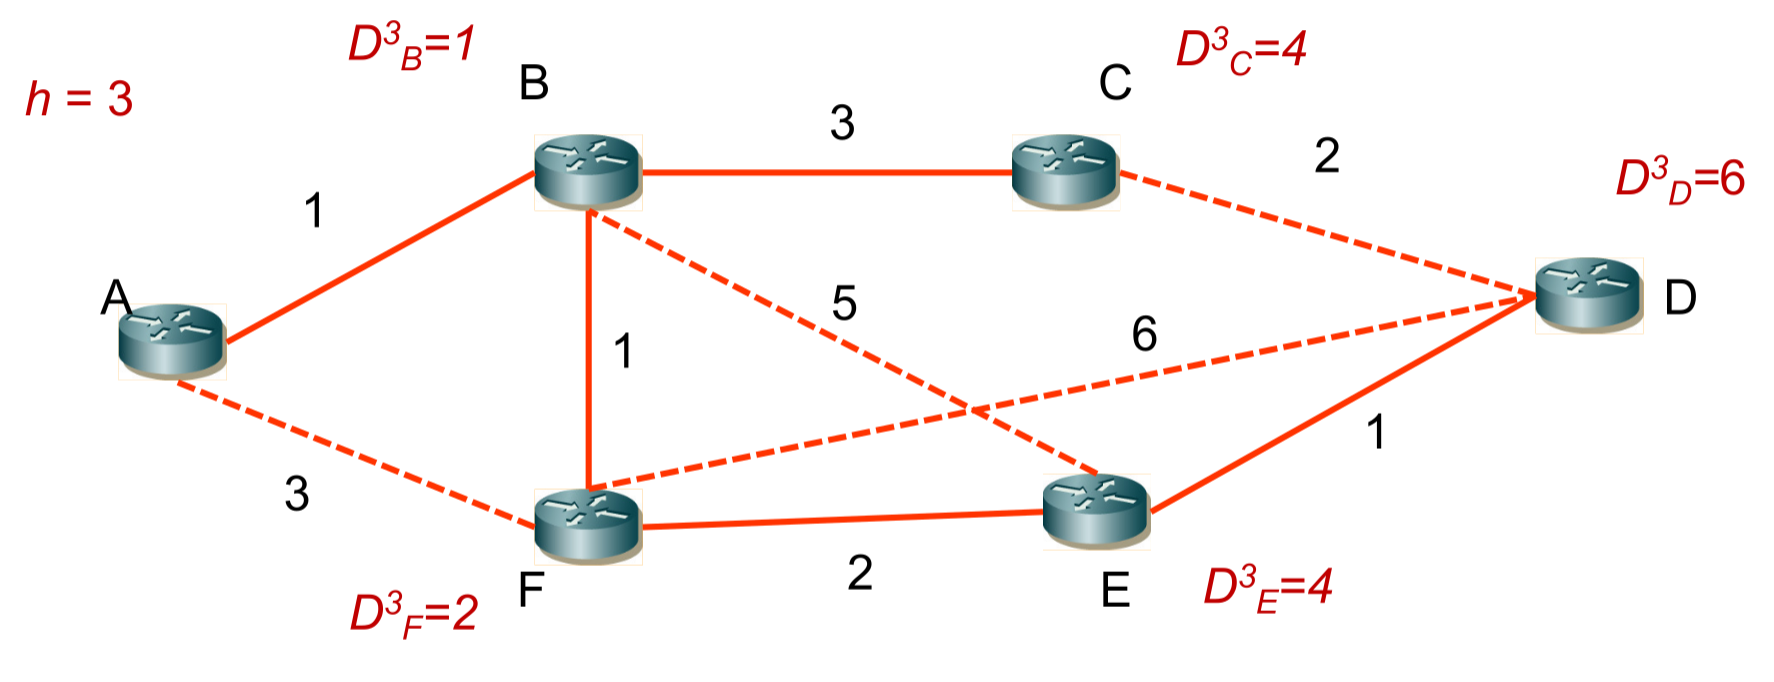
\includegraphics[width=0.85\textwidth]{images/bf4.png}
    \caption{Esempio di applicazione dell'algoritmo di Bellman-Ford - Passo 3}
    \label{fig:bf4}
\end{figure}

\newpage

Poi si calcolano i costi dei cammini quando h = 4

\begin{itemize}
   
    \item $D_B^{(4)}$ =  $\min [0 + 1, 3 + 3, 6 + \infty, 5 + 5, 2 + 1, 1] = 1$
    \item $D_C^{(4)}$ = $\min [0 + 3, 1 + 3, 6 + \infty, 5 + 2, 2 + \infty, 3] = 3$
    \item $D_D^{(4)}$ = $\min [0 + \infty, 1 + \infty, 3 + \infty, 5 + 1, 2 + 5, 6] = 6$
    \item $D_E^{(4)}$ = $\min [0 + \infty, 1 + 5, 3 + 2, 6 + 1, 2 + \infty, 5] = 5$
    \item $D_F^{(4)}$ = $\min [0 + \infty, 1 + 1, 3 + \infty, 6 + 5, 5 + \infty, 2] = 2$
\end{itemize}



\begin{figure}[h!]
    \centering
    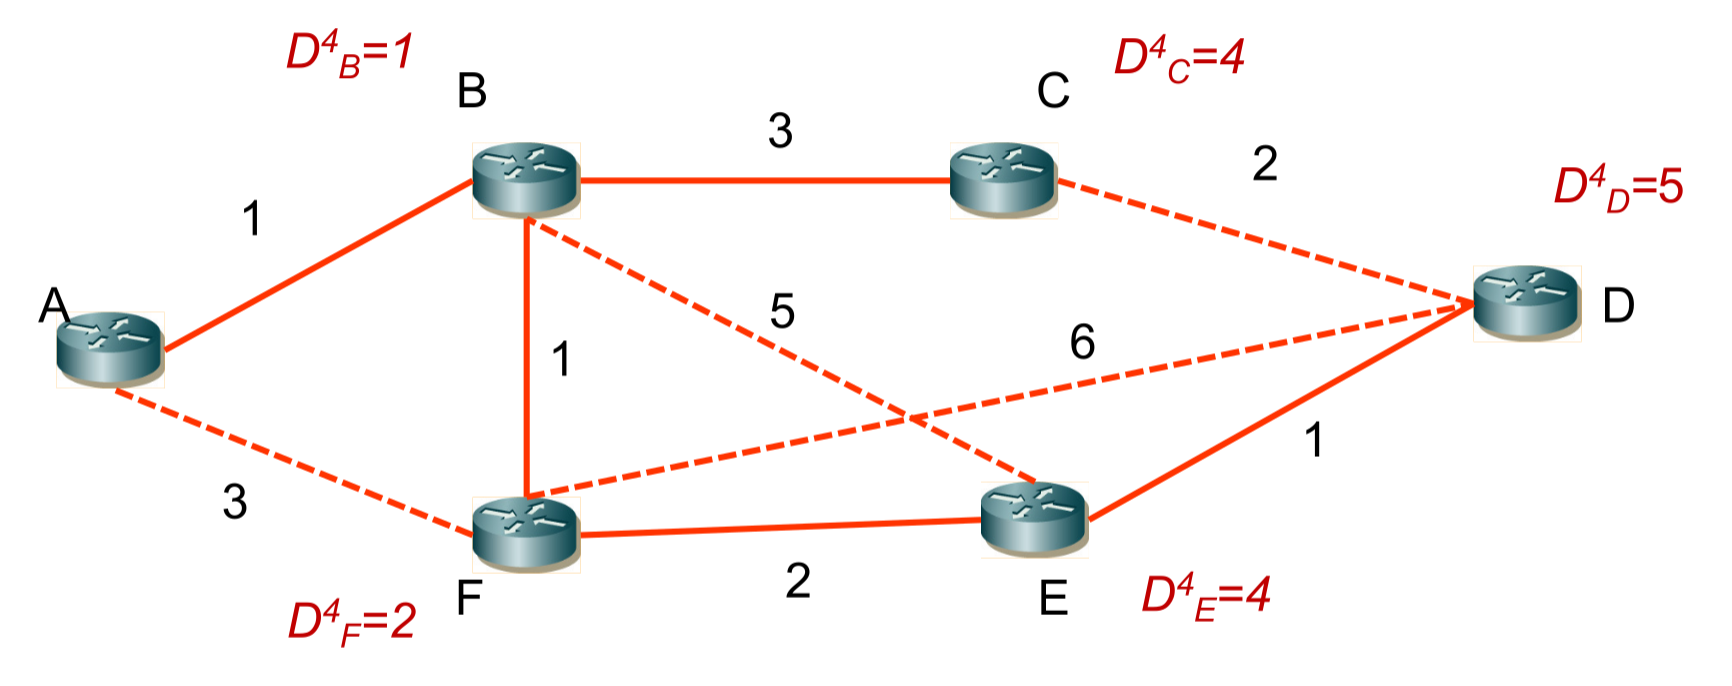
\includegraphics[width=0.7\textwidth]{images/bf5.png}
    \caption{Esempio di applicazione dell'algoritmo di Bellman-Ford - Passo 4}
    \label{fig:bf5}
\end{figure}

\vspace{1em}
\noindent\rule{\linewidth}{0.4pt}
\vspace{1em}


Poi si calcolano i costi dei cammini quando h = 5


\begin{figure}[h!]
    \begin{minipage}{0.6\textwidth}
    \begin{itemize}
   
    \item $D_B^{(5)}$ = $\min [0 + 1, 3 + 3, 6 + \infty, 5 + 5, 2 + 1, 1] = 1$
    
    \item $D_C^{(5)}$ = $\min [0 + 3, 1 + 3, 6 + \infty, 5 + 2, 2 + \infty, 3] = 3$
    
    \item $D_D^{(5)}$ = $\min [0 + \infty, 1 + \infty, 3 + \infty, 5 + 1, 2 + 5, 6] = 6$
    
    \item $D_E^{(5)}$ = $\min [0 + \infty, 1 + 5, 3 + 2, 6 + 1, 2 + \infty, 5] = 5$
    
    \item $D_F^{(5)}$ = $\min [0 + \infty, 1 + 1, 3 + \infty, 6 + 5, 5 + \infty, 2] = 2$
    \end{itemize}

    \end{minipage}\hfill
    \begin{minipage}{0.35\textwidth}
        \begin{center}
                    L'algoritmo si ferma qui poichè i cammini calcolati per h=4 sono identici a quelli calcolati adesso con h=5, perciò stop:

            If $D_j^{h} = D_j^{h-1} \quad \forall j \neq s$

        then $h_{max} = h - 1$; stop
        \end{center}
    \end{minipage}
\end{figure}





\begin{figure}[h!]
    \centering
    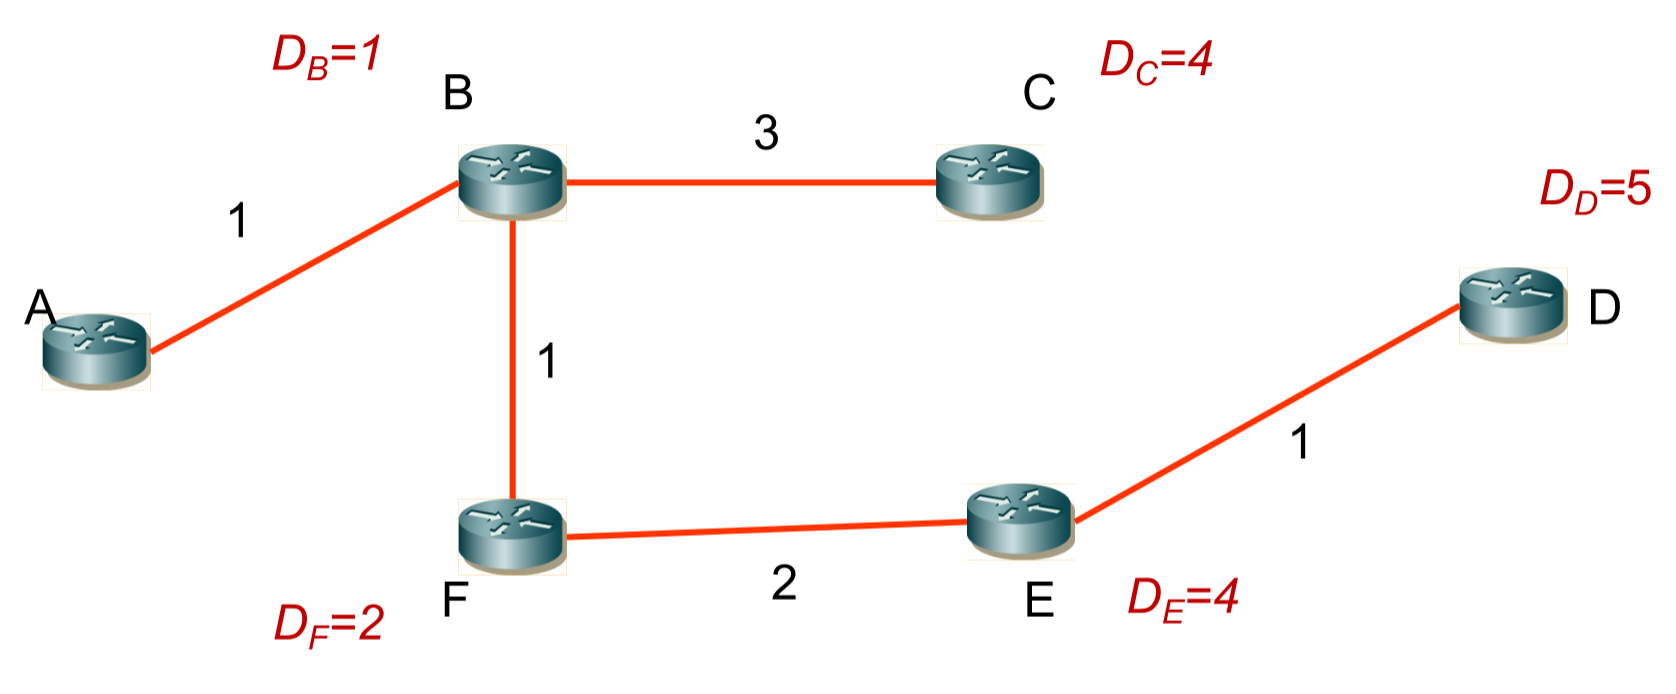
\includegraphics[width=0.7\textwidth]{images/bf7.png}
    \caption{Albero dei cammini a costo minimo}
    \label{fig:bf7}
\end{figure}

\subsection{Link State e Dijkstra}

L'algoritmo link-state rappresenta un'alternativa al vistance vector, si utilizza per reti di dimensioni maggiori.

Il presupposto su cui si basa questo algoritmo è che i router conoscano la topologia della rete, non come avveniva nel distance vector; infatti nel distance vector i router conoscevano solamente le info sui vicini, nel link state invece i router conoscono l'intera topologia della rete.

\paragraph{Flooding(routing senza tabella)}
Si sfrutta il concetto di flooding: il flooding è un protocollo di instradamento usato dai router che inoltrano un pacchetto in ingresso su tutte le linee ad eccezione di quella da cui proviene. Ogni pacchetto in arrivo viene inoltrato su ogni linea di uscita eccetto quella da cui è arrivato;
quindi tutti i router della rete comunicano in flooding tutte le informazioni dei vicini, con relativi costi. Inoltre il link state periodicamente ritrasmette l'informazione.

La topologia della rete è cosa nota a tutti e quindi si possono applicare strategie porprie della teoria dei grafi, più nello specifico applichiamo l'algoritmo di Dijkstra(complessità non lineare, nlog(n), ossia con l'aumetare dei nodi la complessità di questo algoritmo aumenta alla nlog(n)):
permette di trovare la strada nel modo più efficiente possibile(considerando tempo e costo: migliore end to end).


\subsubsection{Algoritmo di Dijkstra}


A differenza dell'algoritmo di Bellman-Ford, quello di Dijkstra viene applicato dai router della rete; ad ogni cambiamento della topologia(o dopo tot tempo) vengono calcolati i cammini minimi.

Considerazioni preliminari:

\begin{itemize}
    \item s è la sorgente, ossia il router da cui si calcolano i cammini minimi usando Dijkstra
    \item N è l'insieme dei nodi della rete
    \item M è l'insieme dei nodi dell'albero corrente
    \item V(M) è l'insieme dei nodi raggiiungibili con un solo salto dai nodi dell'albero M
    \item $D_j$ è il costo del cammino a costo minimo, da s al nodo j
    \item $d_{ij}$ è il costo del collegamento diretto tra i nodi i e j;
    
    se il collegamento non è diretto allora questo costo è infinito
\end{itemize}

Steps dell'algoritmo:
\begin{enumerate}
    \item Inizializzazione: considero l'insieme M pari ad s; 
    


    nel caso in cui il nodo di cui desidero calcolare il cammino sia collegato direttamente ad s, quindi j fa parte dell'insieme V(M), allora il costo del cammino minimo sarà:
    \[
    M = \{s\} \qquad
    D_j = 
    \begin{cases}
        d_{sj}, & \forall j \in V(s) \\
        \infty, & \text{altrimenti}
    \end{cases}
    \]
    \item prendo in considerazione i nodi che fa parte dell'insieme V(M), perciò i nodi vicini a M, raggiungibili con un solo salto;
   scelgo un k nodo che sia il più vicino all'albero M rispetto gli altri nodi vicini, "il più vicino tra i vicini": aggiungo k all'albero M e ne calcolo la distanza per arrivare al nodo j, e la aggiungo nell'insieme con i cammini $D_j$

\[
\text{Select } k \in V(M) \mid D_k = \min_{i \in V(M)} \{ D_i \}  \qquad   M = M \cup \{ k \}  
\]
\[
D_j = \min \{ D_j,\, D_k + d_{kj} \} \qquad \forall\, j \in V(M)
\]
    
   \item si prosegue con il passaggio svolto in precedenza(ricerca del vicino da aggiungere all'albero M) fino a quando non ho ottenuto tutti i cammini minimi, perciò fino a quando l'albero M non sia pari alla rete stessa:
    
If $M = N$ stop,\\
altrimenti vai al passo 2.
\end{enumerate}

\subsubsection{Esempio Dijkstra}

\begin{figure}[h!]
    \begin{minipage}{0.5\textwidth}
        \centering
        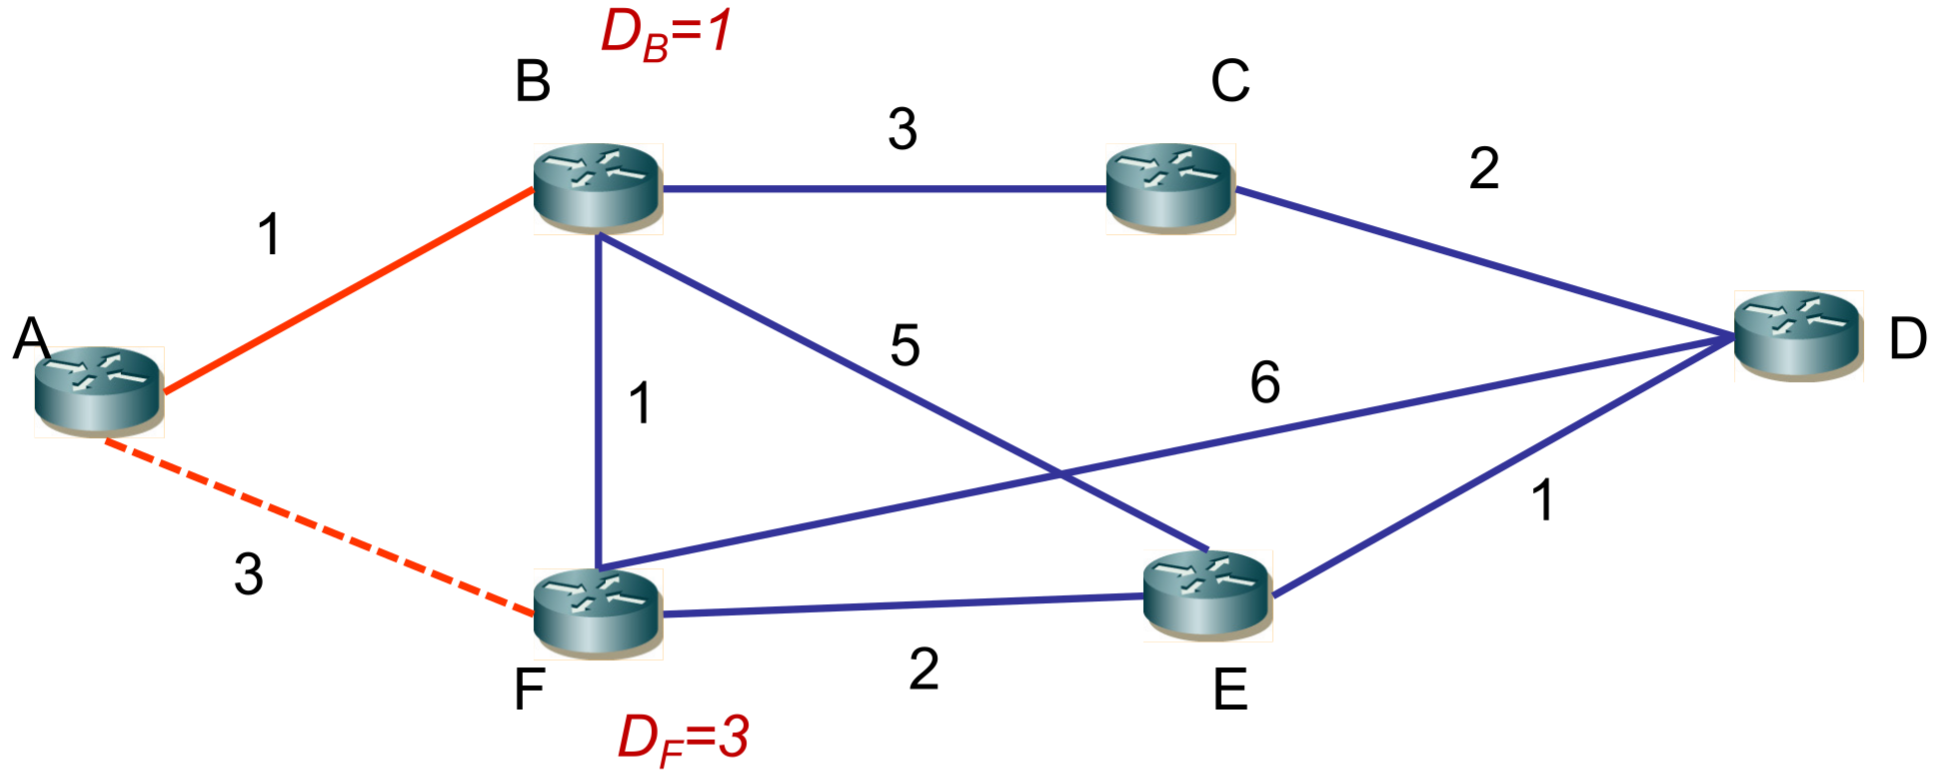
\includegraphics[width=0.95\textwidth]{images/linkstate3.png}
        \caption{Esempio Link State}
        \label{fig:linkstate1}
    \end{minipage}\hfill
    \begin{minipage}{0.49\textwidth}
        \textbf{Passo 1 dell'algoritmo di Dijkstra}

        \[
        M = \{A\}, \quad V(M) = \{B, F\}
        \]

        \[
        D_B = D_A + d_{AB} = 0 + 1 = 1
        \]
        \[
        D_F = D_A + d_{AF} = 0 + 3 = 3
        \]
        B è il nodo diretto più vicino:
        \[
        \min \{ D_B, D_F \} = \min \{ 1, 3 \} = 1 = D_B \implies
        \]
        \[
        M = M \cup B; \quad \mathbf{V(M) = \{C, E, F\}}
        \]
    \end{minipage}
\end{figure}

\begin{figure}[h!]
    \begin{minipage}{0.5\textwidth}
        \centering
        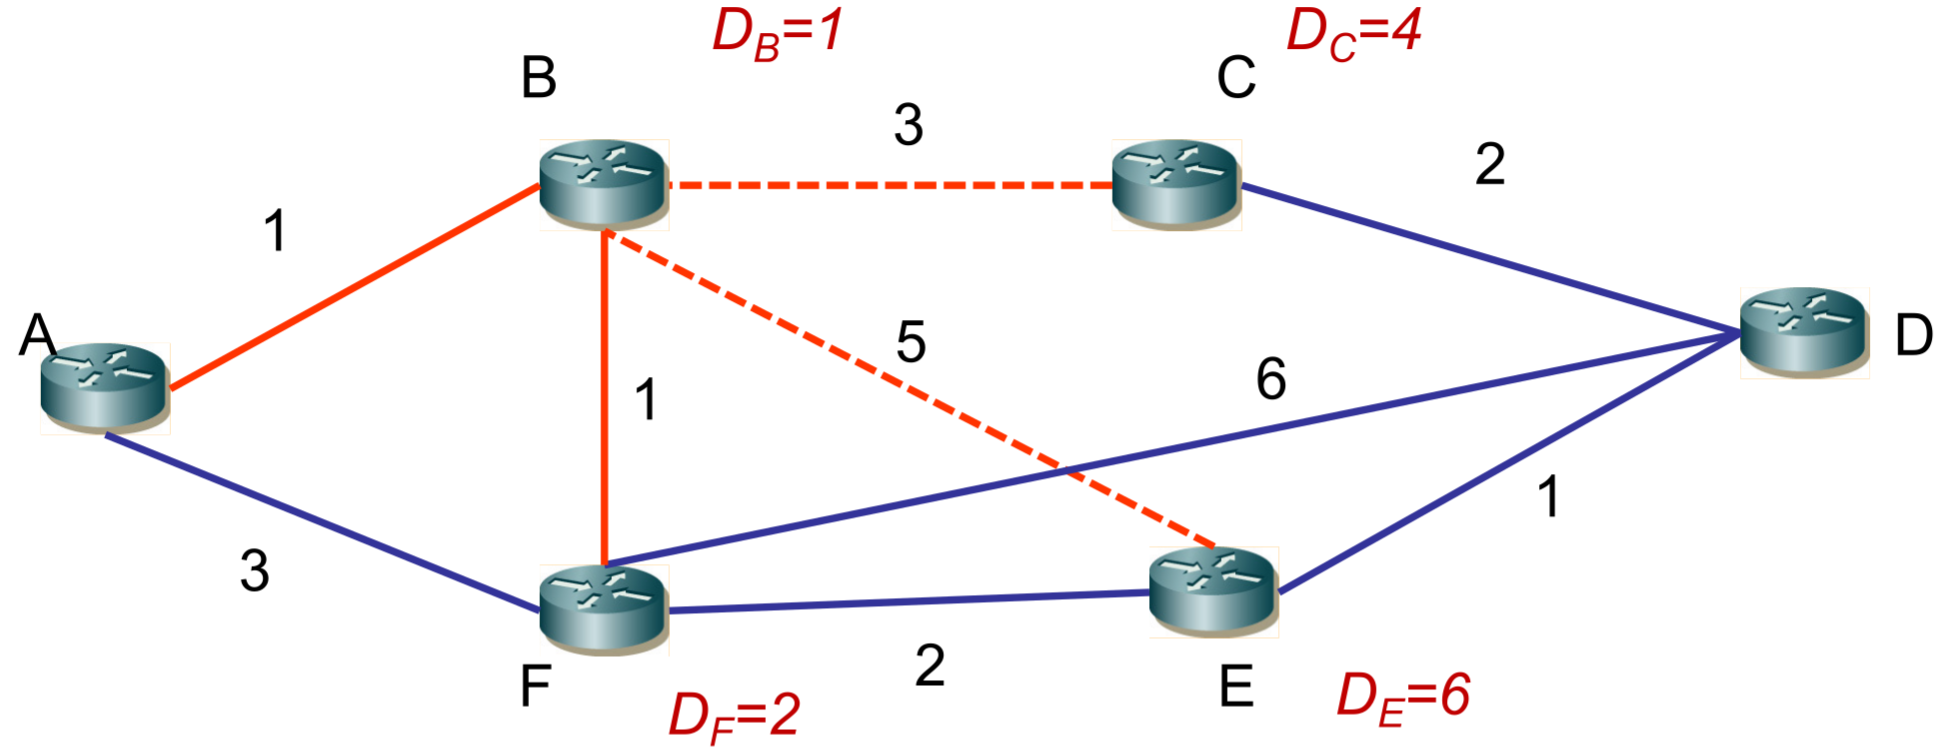
\includegraphics[width=0.95\textwidth]{images/linkstate5.png}
        \caption{Esempio Link State - Passo 2}
        \label{fig:linkstate4}
    \end{minipage}\hfill
    \begin{minipage}{0.49\textwidth}
        \textbf{Passo 2 dell'algoritmo di Dijkstra}

        Ora $M = \{A, B\}$, $V(M) = \{C, E, F\}$.

        \[
        D_C = \min(D_C, D_B + d_{BC}) = \min(\infty, 1 + 3) = 4
        \]
        \[
        D_E = \min(D_E, D_B + d_{BE}) = \min(\infty, 1 + 5) = 6
        \]
        \[
        D_F = \min(D_F, D_B + d_{BF}) = \min(3, 1 + 1) = 2
        \]

        Il nodo più vicino è $F$ ($D_F = 2$), quindi 
        
        $M = \{A, B, F\}$.
    \end{minipage}
\end{figure}

\begin{figure}[h!]
    \begin{minipage}{0.5\textwidth}
        \centering
        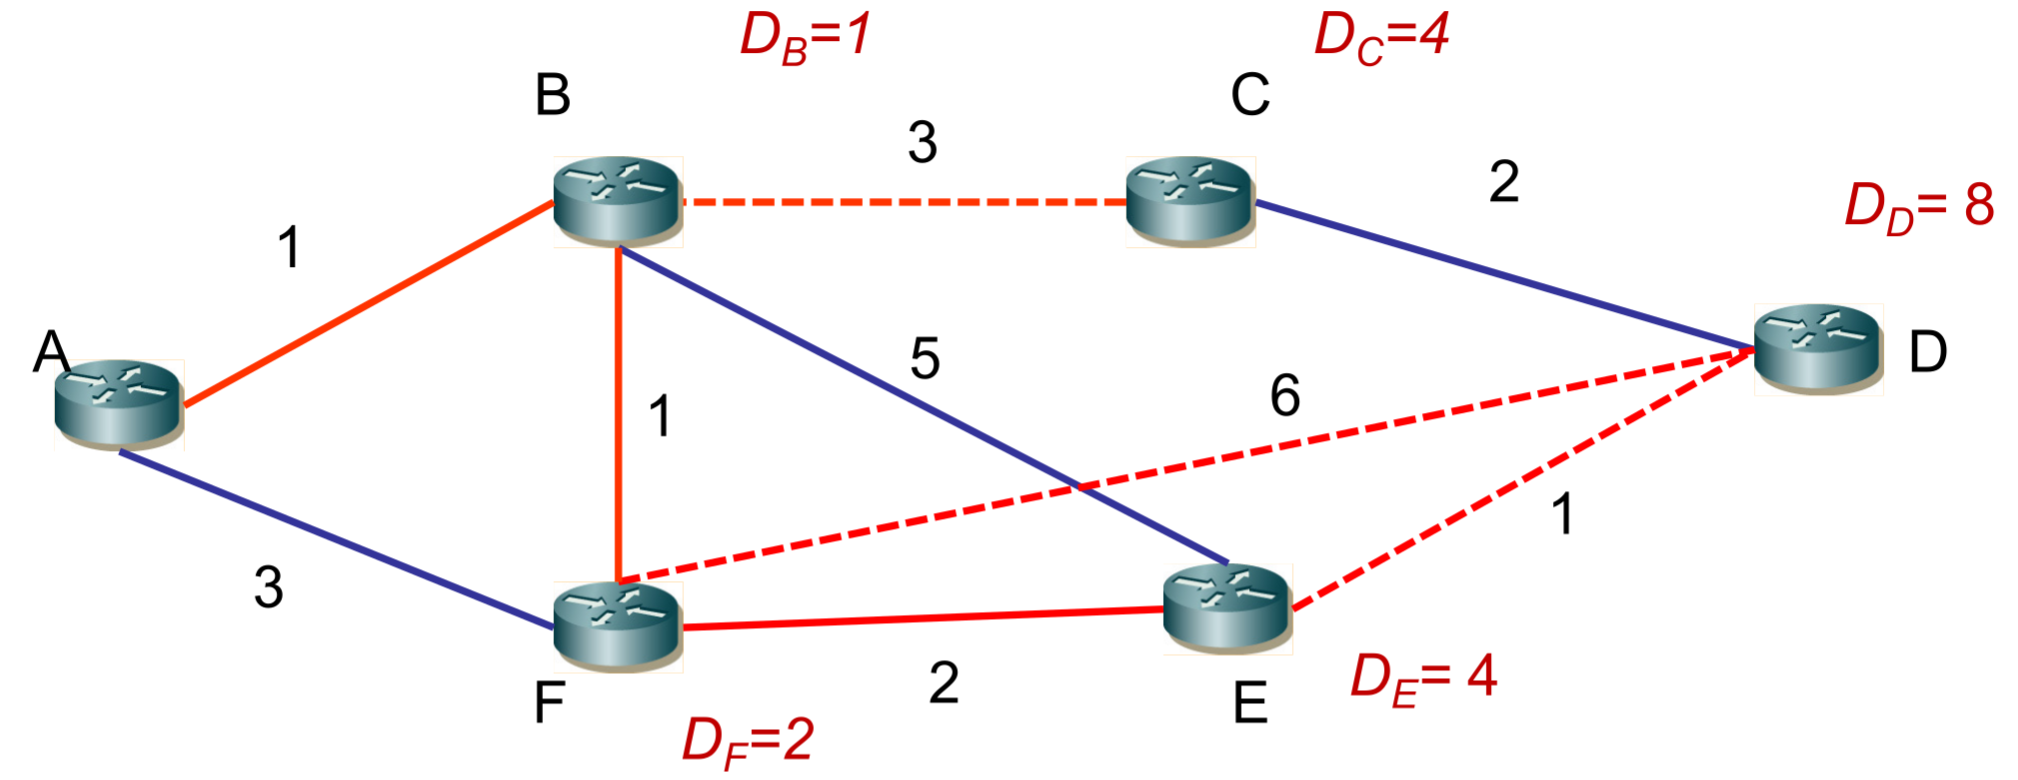
\includegraphics[width=0.95\textwidth]{images/linkstate7.png}
        \caption{Esempio Link State - Passo 3}
        \label{fig:linkstate6}
    \end{minipage}\hfill
    \begin{minipage}{0.49\textwidth}
        \textbf{Passo 3 dell'algoritmo di Dijkstra}

        \[
        M = \{A, B, F\}, \quad V(M) = \{C, D, E\}
        \]

        \[
        \begin{aligned}
        D_C &= \min\{ D_C,\, D_F + d_{FC} \} = \min\{4,\, 2 + \infty\} = 4 \\
        D_D &= \min\{ D_D,\, D_F + d_{FD} \} = \min\{\infty,\, 2 + 6\} = 8 \\
        D_E &= \min\{ D_E,\, D_F + d_{FE} \} = \min\{6,\, 2 + 2\} = 4 \\
        \end{aligned}
        \]

        Il nodo più vicino è $C$ o $E$ (entrambi con costo 4). Si può scegliere uno dei due, ad esempio $E$.
    \end{minipage}
\end{figure}

\newpage

\begin{figure}[h!]
    \begin{minipage}{0.5\textwidth}
        \centering
        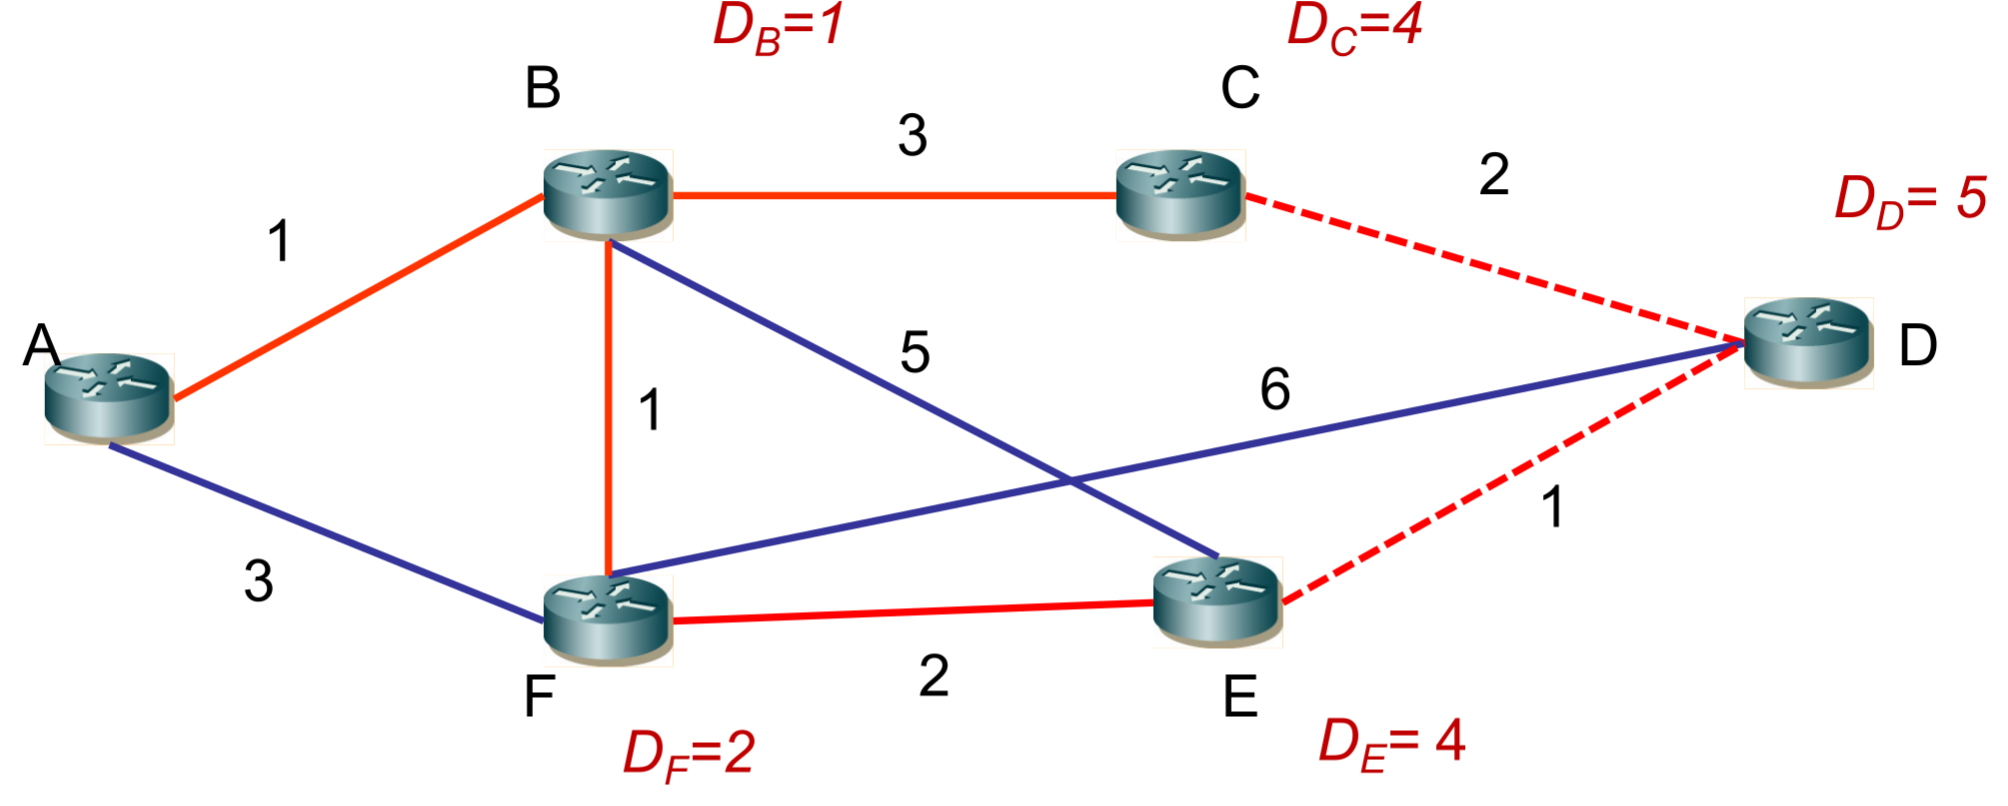
\includegraphics[width=0.95\textwidth]{images/linkstate10.png}
        \caption{Esempio Link State - Passo 4}
        \label{fig:linkstate9}
    \end{minipage}\hfill
    \begin{minipage}{0.49\textwidth}
        \textbf{Passo 4 dell'algoritmo di Dijkstra}

        Ora $M = \{A, B, F, E\}$, $V(M) = \{C, D\}$.

        \[
        \begin{aligned}
        D_C &= \min\{ D_C,\, D_E + d_{EC} \} = \min\{4,\, 4 + \infty\} = 4 \\
        D_D &= \min\{ D_D,\, D_E + d_{ED} \} = \min\{8,\, 4 + 1\} = 5 \\
        \end{aligned}
        \]

        Il nodo più vicino è $C$ ($D_C = 4$), quindi 
        
        $M = \{A, B, C, E, F\}$.
    \end{minipage}
\end{figure}

\begin{figure}[h!]
    \begin{minipage}{0.5\textwidth}
        \centering
        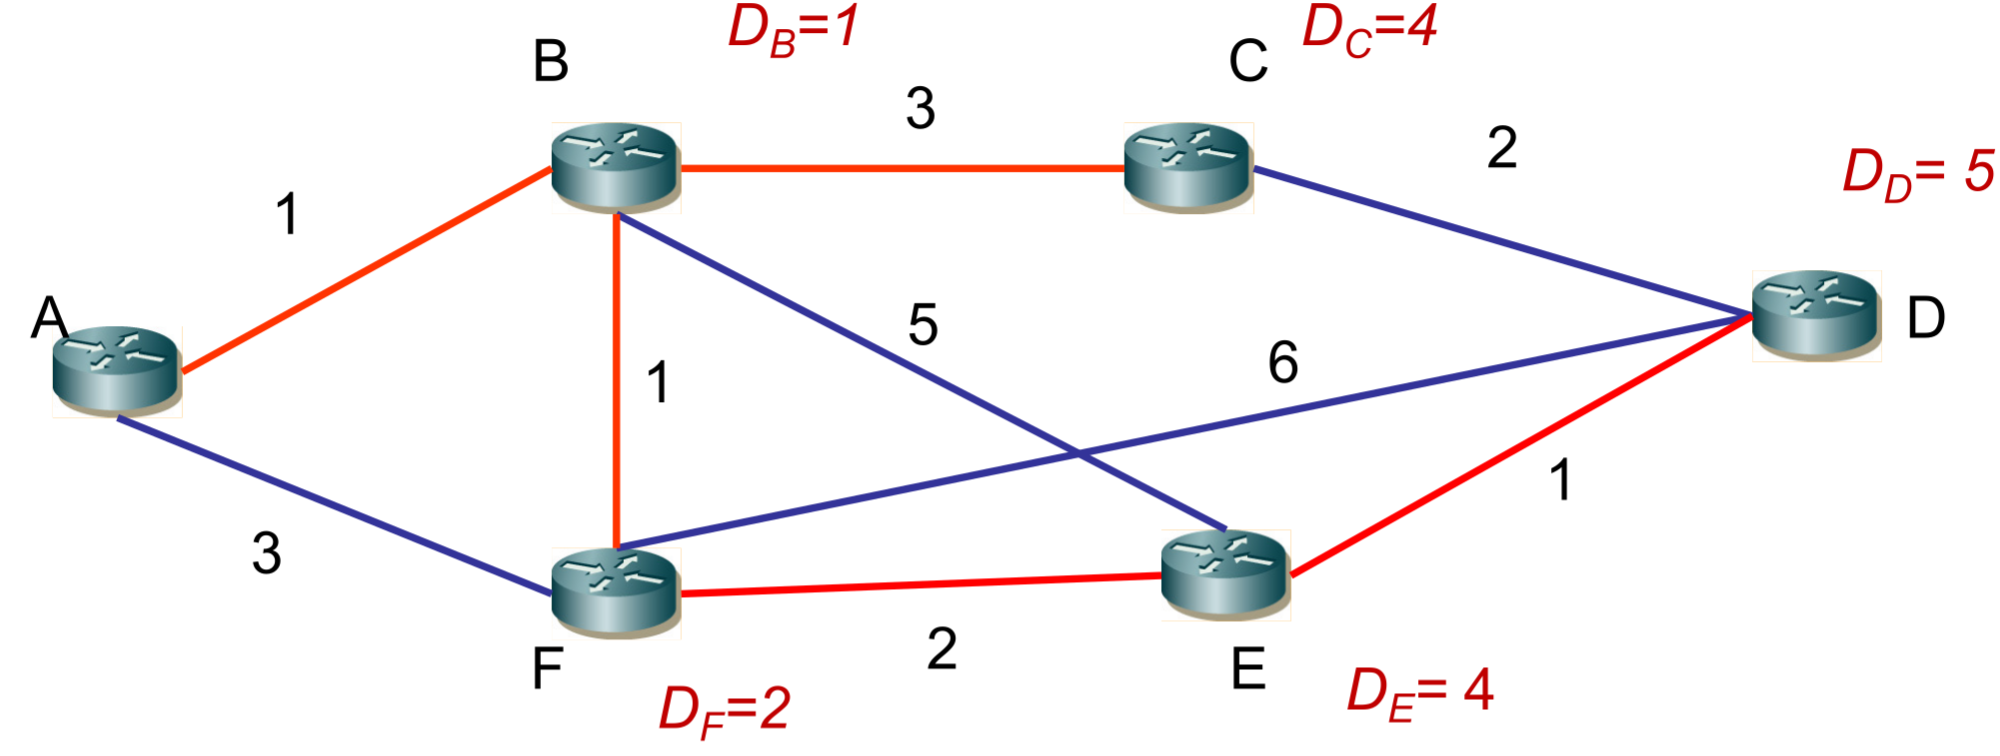
\includegraphics[width=0.95\textwidth]{images/linkstate12.png}
        \caption{Esempio Link State - Passo 5}
        \label{fig:linkstate11}
    \end{minipage}\hfill
    \begin{minipage}{0.49\textwidth}
        \textbf{Passo 5 dell'algoritmo di Dijkstra}

        Ora $M = \{A, B, C, E, F\}$, $V(M) = \{D\}$.

        \[
        D_D = \min\{ D_D,\, D_C + d_{CD},\, D_E + d_{ED} \} = 
        \]
        \[
        \min\{5,\, 4 + 2,\, 4 + 1\} = 5
        \]
        L'albero dei cammini M è stato completato: 
        \begin{center}
            M = N
        \end{center}    
        \[
        \mathbf{M} = \{A, B, C, D, E, F\}, \quad \mathbf{V(M)} = \varnothing
        \]\end{minipage}
\end{figure}

\subsubsection{Albero dei cammini minimi}
Il risultato è identico a quello ottenuto con Bellman-Ford

\begin{figure}[h!]
    \centering
    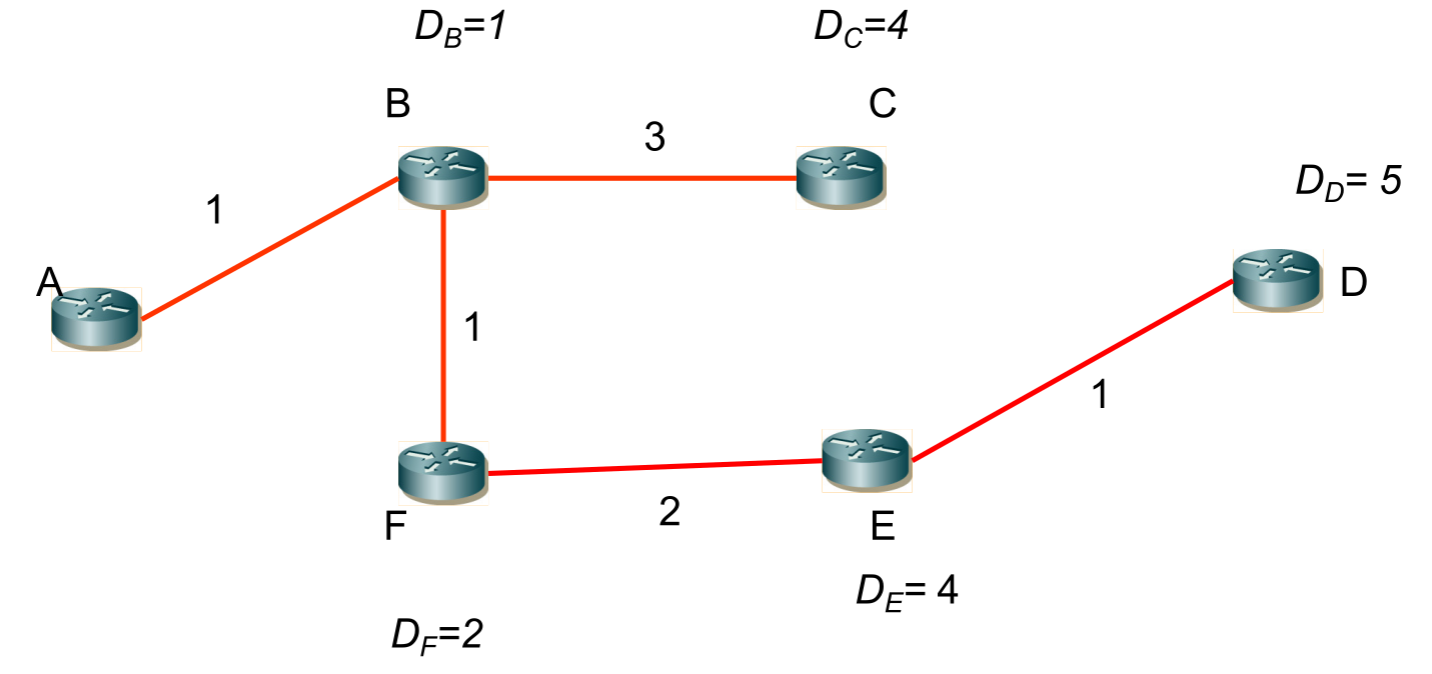
\includegraphics[width=1\textwidth]{images/linkstate134.png}
    \caption{Albero dei cammini}
    \label{fig:alberocammini}
\end{figure}


\newpage

\subsection{Problemi di routing}
Tabelle di routing inziali, rispettivamente, da sinistra, Pippo, Pluto e Topolino; 

con quarta destinazione l'host 192.168.40.0

\begin{figure}[h!]
    \centering
    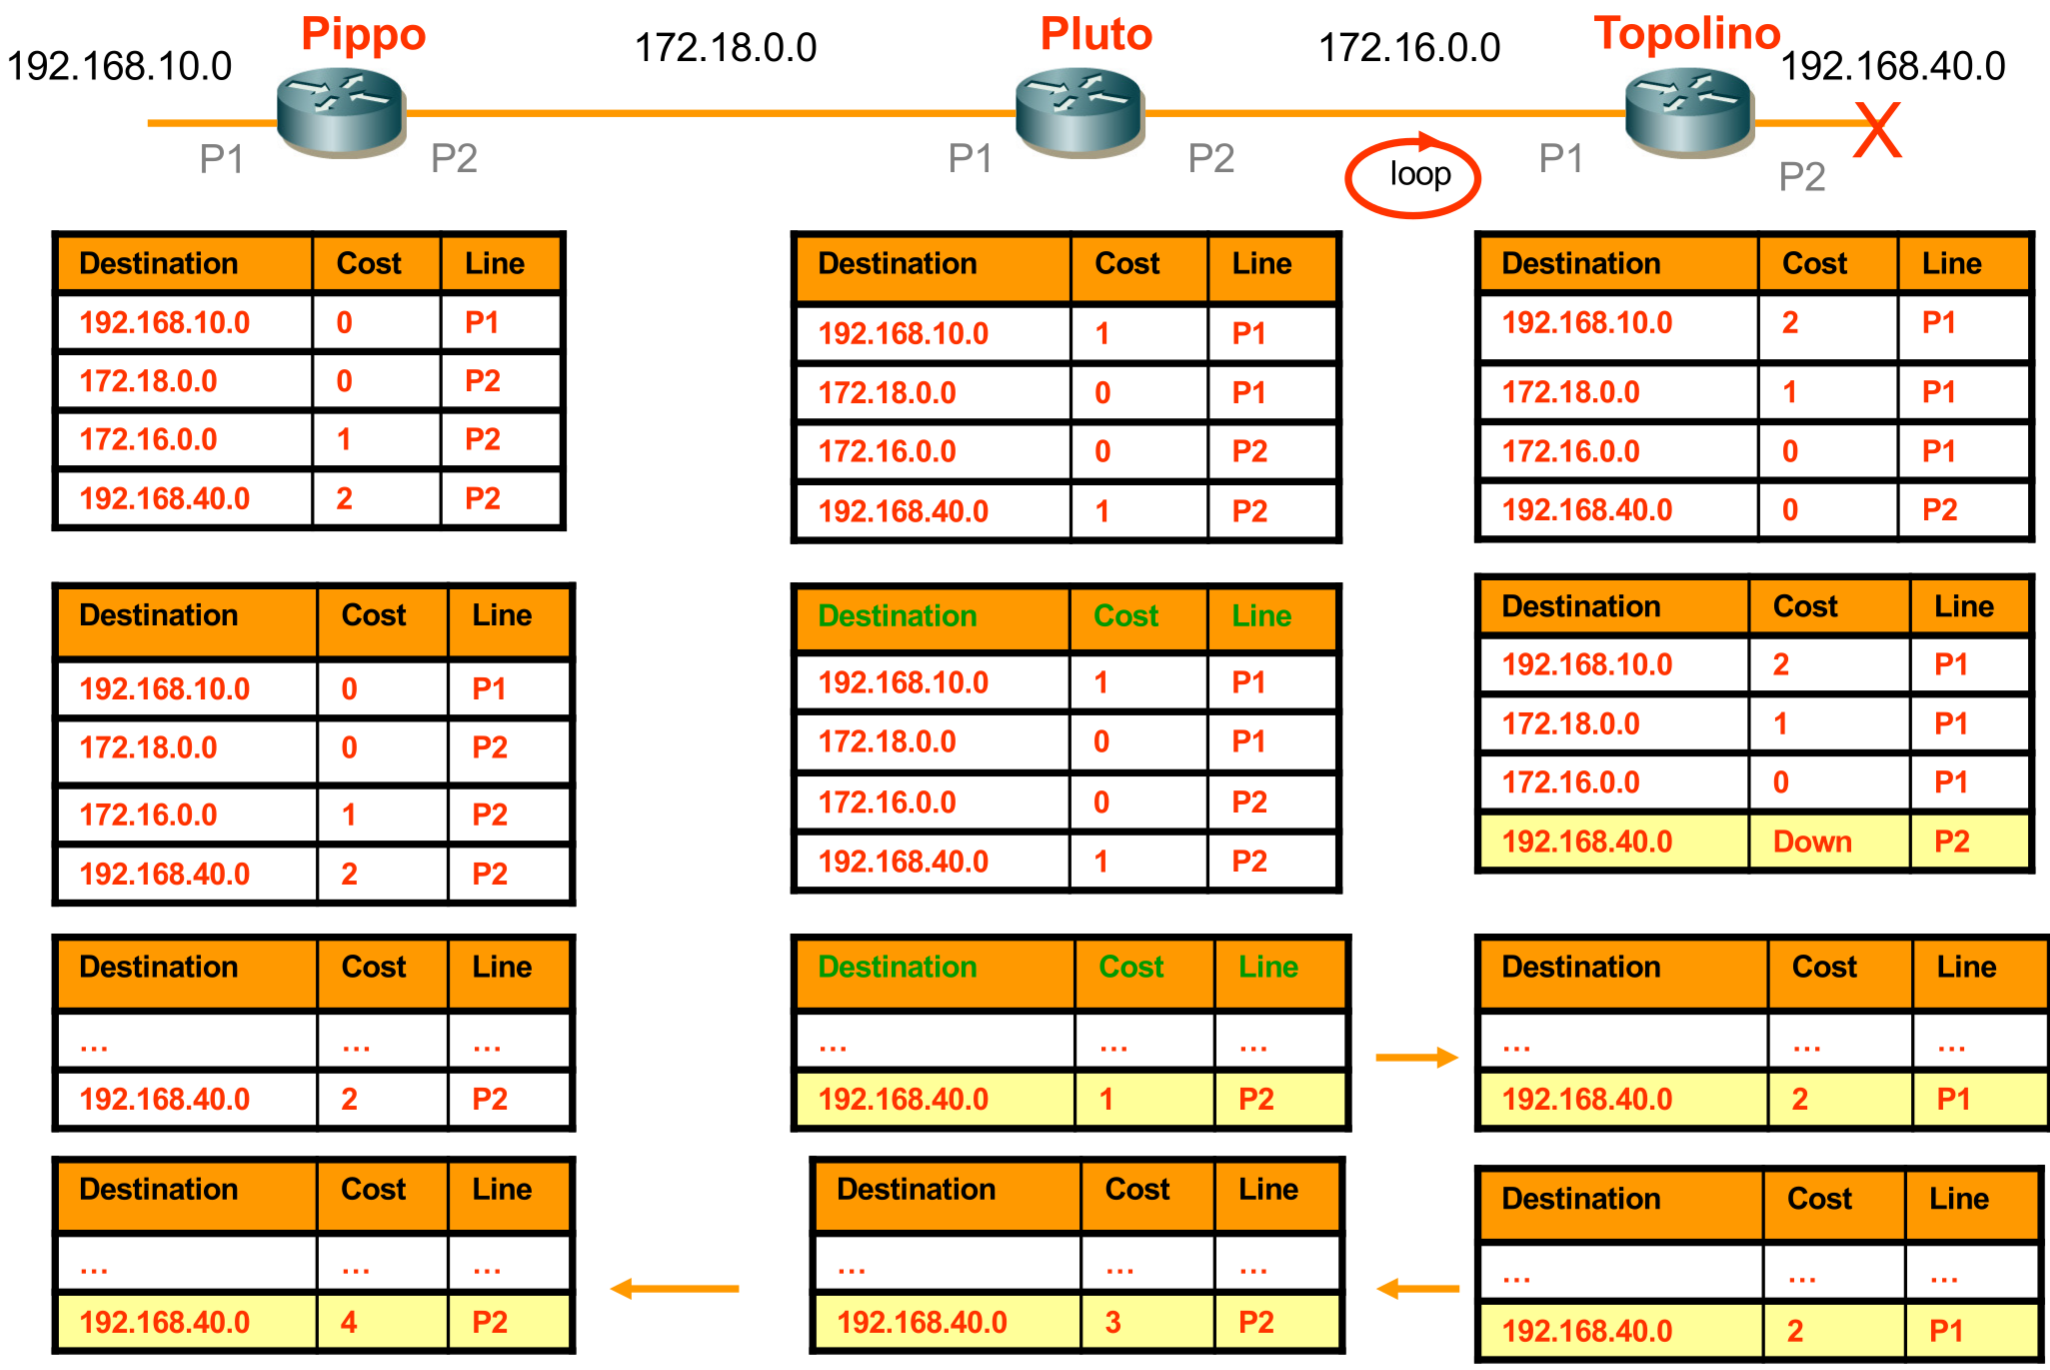
\includegraphics[width=1\textwidth]{images/problemaloop.png}
    \caption{Esempio di tabelle routing}
    \label{fig:problemaloop}
\end{figure}

\vspace{0.5em}
\noindent\rule{\linewidth}{0.4pt}
\vspace{0.5em}

\paragraph{Una rete va giù (down)} ad un certo punto la rete 192.168.40.0 va down e diventa irraggiungibile, questa cosa viene riscontrata solo dalla rete che ha il collegamento diretto, quindi se ne accorge solo Topolino, che inserisce nella tabella "Down".

\begin{figure}[h!]
    \centering
    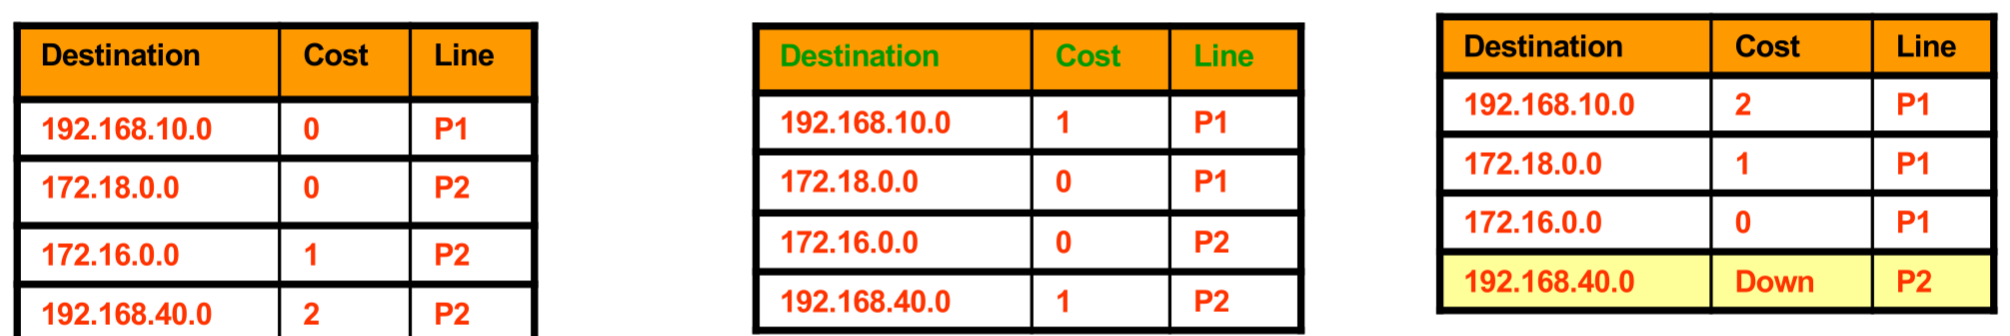
\includegraphics[width=1\textwidth]{images/loop1.png}
    \caption{Una rete va down}
    \label{fig:problemaloop1}
\end{figure}

\vspace{0.5em}
\noindent\rule{\linewidth}{0.4pt}
\vspace{0.5em}

\paragraph{Inizio del loop} la rete topolino, che riscontra la rete in down, cerca di collegarsi a 192.168.40.0 tramite altre router che ne hanno l'accesso;

quindi legge da Pluto che 192.168.40.0 è raggiungibile con un hop, quindi scrive nella propria tabella che la rete down è raggiungibile tramite il passaggio da Pluto, quindi con 2 hop.

\begin{figure}[h!]
    \centering
    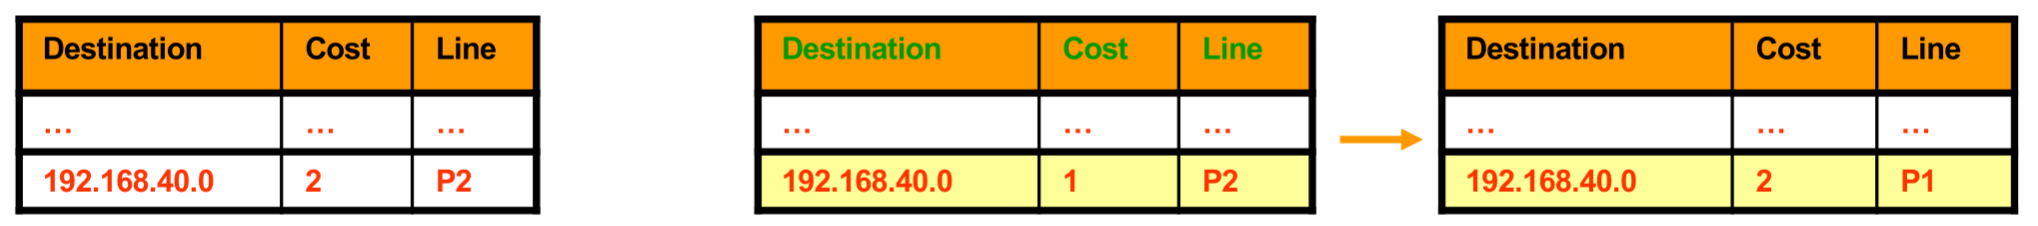
\includegraphics[width=1\textwidth]{images/loop2.png}
    \caption{Inizio del loop}
    \label{fig:problemaloop2}
\end{figure}

\newpage
\paragraph{Loop infinito}
Lo stesso ragionamento fatto precedentemente da Topolino verrà fatto da Pluto, a sua volta verrà fatto anche da Pippo, incrementando infinitamente, un passo alla volta, gli hop necessari a raggiungere una rete che di fatto è irraggiungibile.
\begin{figure}[h!]
    \centering
    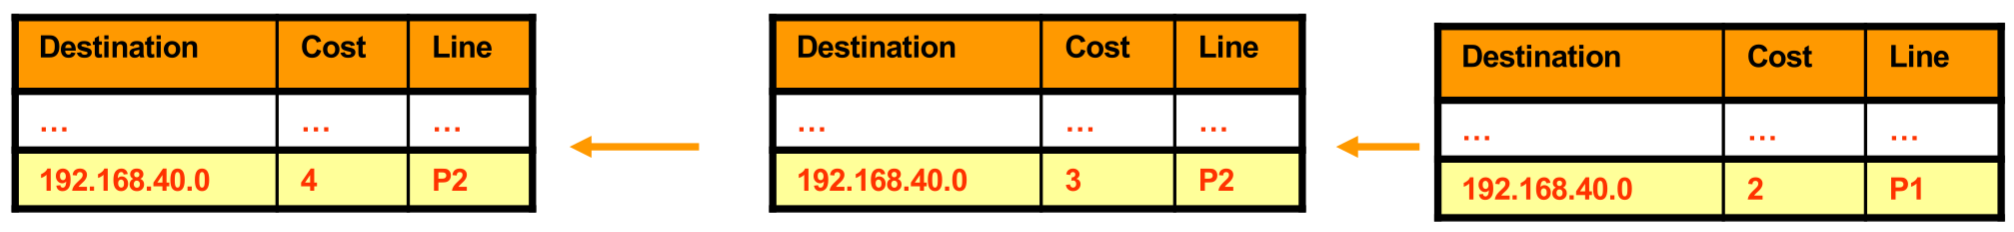
\includegraphics[width=1\textwidth]{images/loop3.png}
    \caption{Loop infinito}
    \label{fig:problemaloop3}
\end{figure}

\subsubsection{Soluzioni: split horizon, poison reverse, hold-down}
La definizione di un massimo blocca il “Counting to infinity”, per evitare il loop si possono usare queste strategie:
\begin{itemize}
    \item Tramite split horizon decido che i router non condividono con i vicini le informazioni ottenute da altri vicini
    \item split horizon con poisoned reverse, invece di non comunicare ai vicini le info di altri vicini, gliele comunico con costo infinito, metrica “infinity”, così che non vengano mai scelte poichè irraggiungibili
    \item trigger update: ogni volta che avviene un cambiamento nella topologia della rete allora vengono aggiornate le tabelle in base a questo cambiamento 
le reti vengono dichiarate irraggiungibili non nell'esatto momento in cui non sono più raggiungibili, ma allo scadere di un time “hold-down timer” 
\end{itemize}

\vspace{0.5em}
\noindent\rule{\linewidth}{0.4pt}
\vspace{0.5em}

\subsection{Protocolli di routing intra AS (RIP - OSPF)}
\subsubsection{RIP (Distance Vector)(UDP)}
\paragraph{Caratteristiche principali}
Il RIP è il protocollo di routing più semplice ed è adatto a reti di piccole dimensioni; usa il Distance Vector.

Come metrica del costo utilizza l'hop count, ossia valuta il costo dei percorsi in base al numero dei santi che vengono effettuati.
Il valore massimo di hop è 15, perciò quando questo valore arriva a 16 per un certo percorso, questo viene indicato come irrangiungibile(per evitare il counting to inifinity).
Il routing update(aggiornamento delle tabelle contenenti le informazioni per il routing) avviene ogni 30s oppure ad ogni cambiamento topologico.

\newpage


\paragraph{RIPv1 e RIPv2}

 Nel RIPv1 l'indirizzamento IP era classful, perciò i pacchetti scambiati non contenevano informazioni sulla maschera di rete; quindi come destinazione si scriveva solamente l'ind. IP.

 RIPv2 invece ha integrato anche la riga Subnet Mask, così da permettere l'uso degli indirizzi classless. 

 I messaggi RIP vengono incapsulati all'interno di UDP(porta 520), perciò tramite datagrammi. Ognuno di questi pacchetti può contenere al massimo 25 destinazioni.

\begin{figure}[h!]
    \centering
    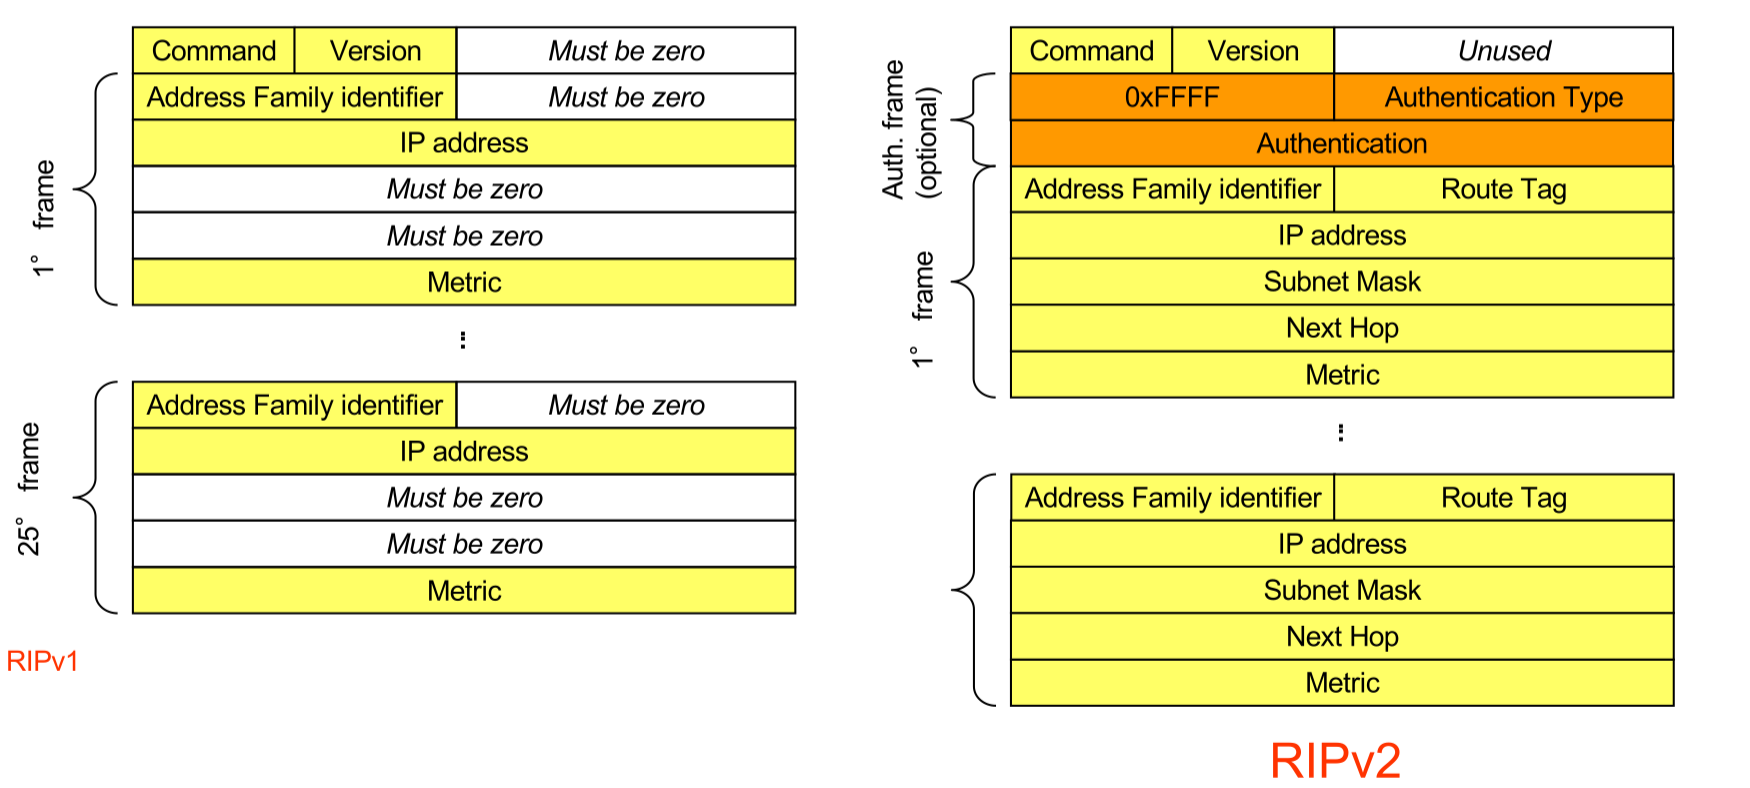
\includegraphics[width=1\textwidth]{images/RIPversioni.png}
    \caption{Confronto tra RIPv1 e RIPv2}
    \label{fig:ripversioni}
\end{figure}

\begin{figure}[h!]
    \centering
    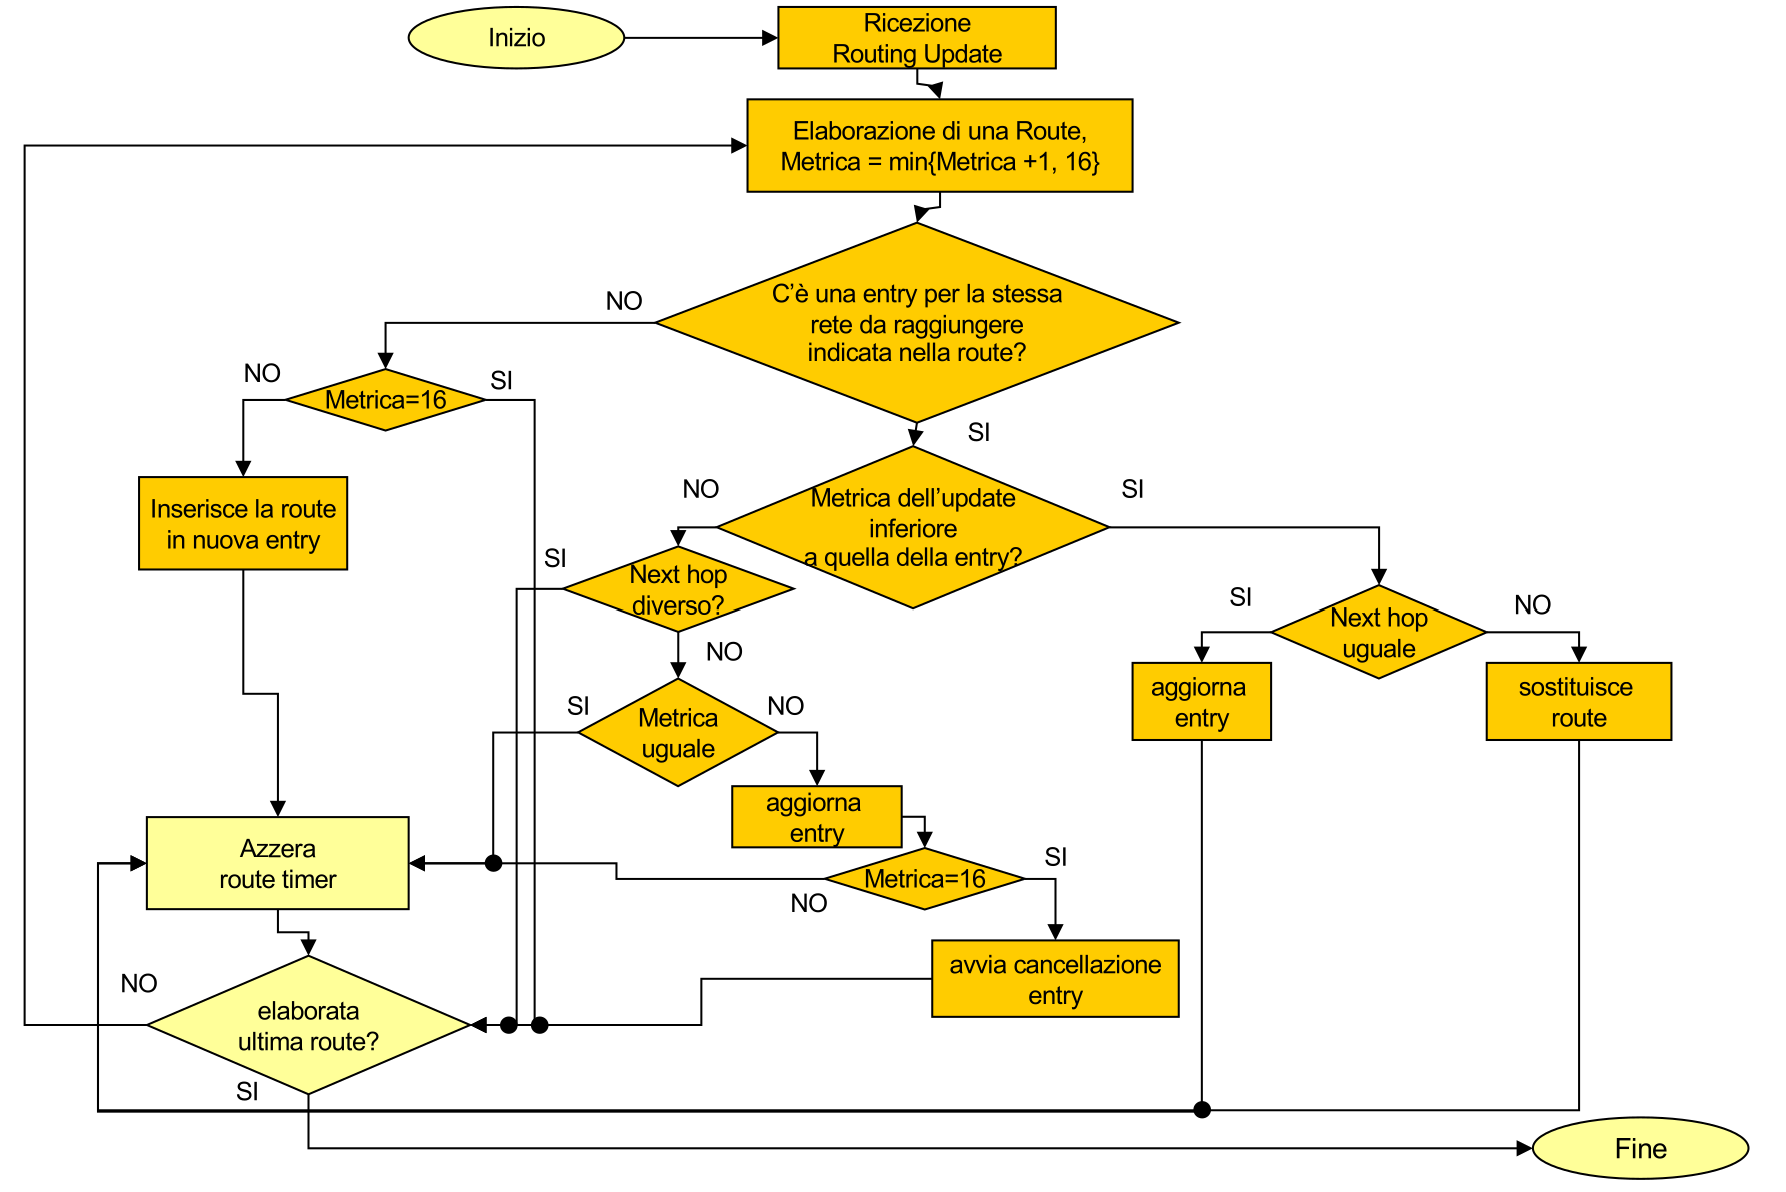
\includegraphics[width=1\textwidth]{images/processoRIP.png}
    \caption{Processo di aggiornamento in RIP}
    \label{fig:processoRIP}
\end{figure}
\newpage
\subsubsection{OSPF (Link State) e Link State Advertisement (LSA)}

Un protocollo che utilizza il link state come alg di routing è il OSPF(open shortest path first);
in OSPF si può specificare quale sia il costo(banda, affidabilità, ritardo, anche un valore inserito manualmente).

Quando i router diventano tanti allora OSPF non fa altro che dividere gli AS in aree, ognuna delle quali definita da 4 ottetti, in modo gerarchico;
\paragraph{Area border routers}
i router al confine con due aree vengono detti “area border router” e devono avere almeno un'interfaccia verso la backbone area(rete 0.0.0.0)
questa backbone area(area 0) fa da ponte tra le aree.
L'idea è quella di usare l'algoritmo dijkstra in ogni singola area e non sul totale, così da richiedere meno dispendio compilativo.

\paragraph{LSA e pacchetti LSP}
I Link State Packet: sono pacchetti generati dal protocollo OSPF, contengono i vari nodi a cui il router è collegato, informazione contenuta nel campo LSA(Link State Advertisement).

Nella rete locale LAN è importante definire un router che inoltri i pacchetti LSP, questo router viene chiamato “designated” router.

Per ridurre l'overhead(risorse richieste in sovrappiù rispetto a quelle strettamente necessarie) da segnalazione, l'LSP viene inviato ogni 30 minuti o ad ogni qual volta ci sia un cambiamento dei collegamenti della rete.

\paragraph{Tipologie di pacchetti LSP}
I pacchetti LSP sono utilizzati per scambiare informazioni tra i router OSPF e sono di tre tipi:
\begin{itemize}
    \item link state request: richiesta di invio di uno o più LSA
    \item link state update: ogni 30 min o quando avviene un cambiamento topologico
    \item link state acknowledgment: all'avvenuta ricezione del LSA
\end{itemize}
\paragraph{Tipologie di LSA}
In OSPF esistono cinque tipologie di LSA, che vengono utilizzate per scambiare informazioni sulla topologia della rete tra i router OSPF:
\begin{multicols}{2}
\begin{itemize}
    \item router LSA
    \item Network LSA
    \item Summary LSA
    \item AS Boundary
    \item router LSA
    \item AS external LSA
\end{itemize}
\end{multicols}
! un LSA “vecchio” di circa un'ora viene rimosso
\begin{figure}[h!]
    \centering
    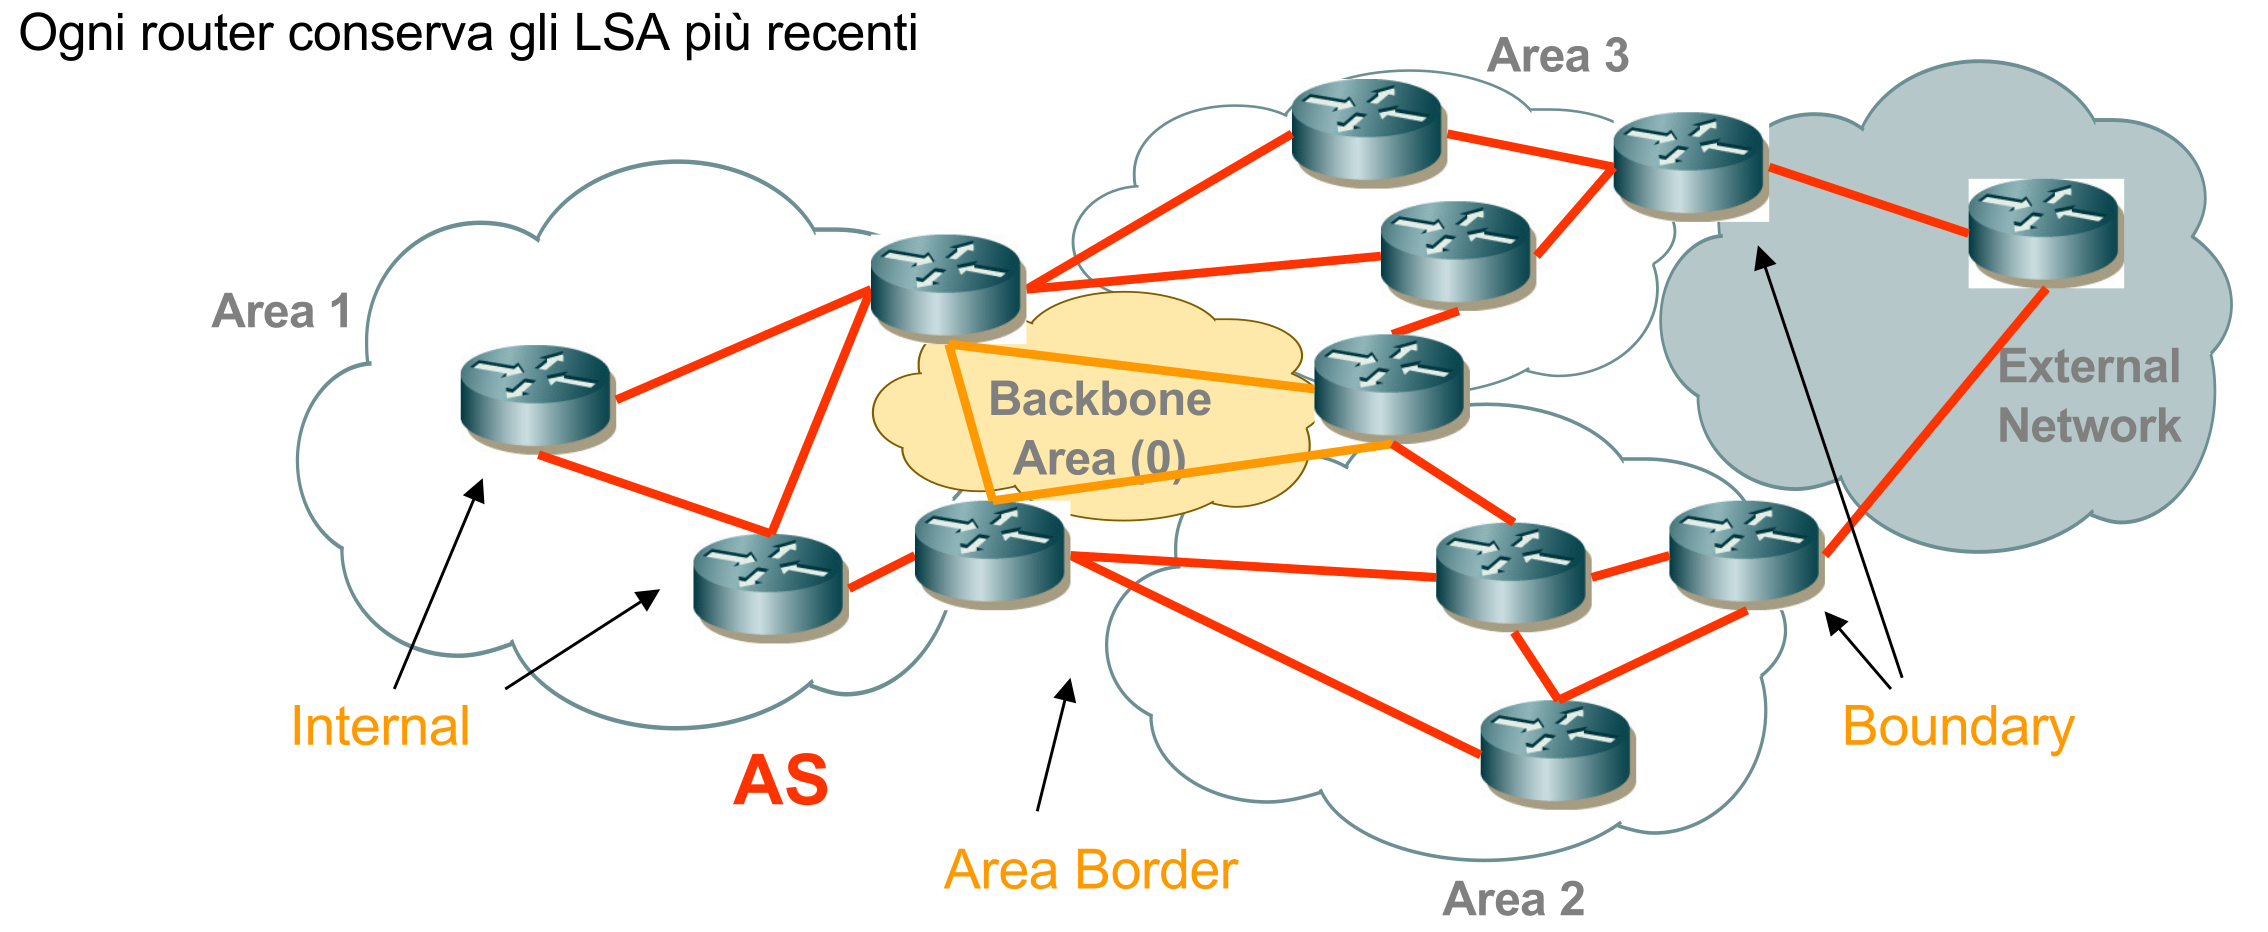
\includegraphics[width=0.82\textwidth]{images/backbone.png}
    \caption{Backbone della rete OSPF}
    \label{fig:backbone}
\end{figure}

\newpage
\paragraph{Differenza tra LSA e pacchetto OSPF}
LSA è informazione vera e propria dello stato dei link.
Il pacchetto OSPF invece trasporta una o più LSP tra router che utilizzano OSPF.
\paragraph{Autenticazione}
OSPF supporta l'autenticazione dei pacchetti, per garantire che i pacchetti OSPF siano inviati da router autorizzati e non siano stati manomessi.
Si distinguiono due tipi di autenticazione:
\begin{itemize}
    \item \textbf{Autenticazione del peer}: verifica che il pacchetto sia inviato da un router autorizzato
    \item \textbf{Autenticazione del messaggio}: verifica l'integrità del messaggio stesso, assicurandosi che non sia stato alterato durante la trasmissione
\end{itemize}
\paragraph{Pacchetto OSPF}
Il pacchetto OSPF è incapsulato in pacchetti IP(type 59, in esadecimale).

Del pacchetto OSPF mi serve sapere: version, Router ID(IP address del router), Area ID, link state checksum.


\paragraph{Utilizzo di Dijkstra in diverse aree}
Ad esempio, nell'area 1 uso il dijkstra tra quei 4 router, i rouer di bordo area avranno sicuramente dei collegamenti con le altre aree, però durante il calcolo dijkstra in area 1 questi altri collegamenti “terminano” sui router di bordo area. 
questo ragionamento viene applicato ad ogni area, anche alla backbone area, che mi va a risolvere il fatto che i router di bordo area precedentemente non integravano nel dijkstra i collegamenti fuori dalla prorpia area. così ho calcolato le strade più efficienti di ogni area, il che porta a vantaggi anche nel quadro globale della cosa.
ci sono anche router detti boundary router che si collegano con “internet”, con il “mondo esterno”, infatti tutte le aree precedenti fanno parte della stessa rete, è divisa solo in aree.
così abbasso il costo computazionale dell'algoritmo dijkstra perchè non lo applico a tutta la rete, ma a tutte le aree che compongono la rete, poichè è un algoritmo la cui complessità è nlog(n), perciò meglio usarlo più volte con un numero inferiore di nodi(n) che una sola volta con un numero  elevato di n

\subsubsection{Pacchetti OSPF}

\begin{figure}[h!]
    \centering
    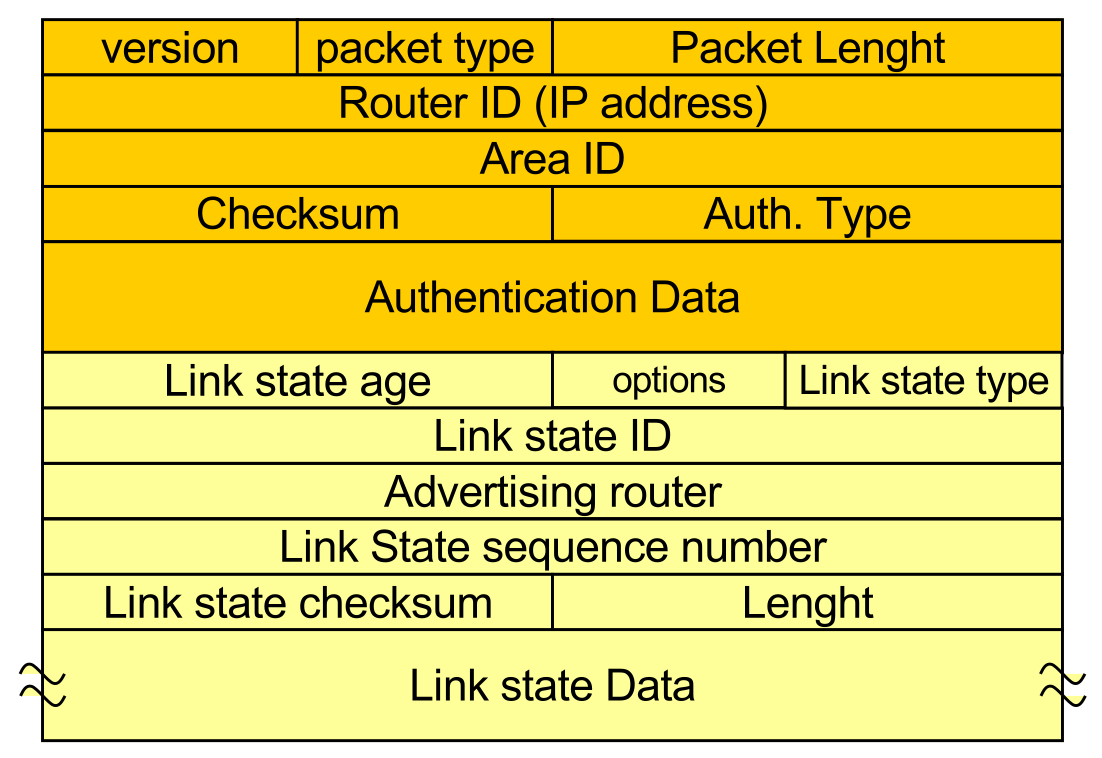
\includegraphics[width=0.7\textwidth]{images/pacchettoospf.png}
    \caption{Pacchetto OSPF}
    \label{fig:pacchettoospf}
\end{figure}

\subsection{Protocolli di routing inter-AS - (BGP)}
Il BGC(border gateway protocol) è il protocollo che gestisce il routing tra AS diversi, è montato sui router di frontiera degli AS.

Esistono tre tipologie di Autonomous Systems:  
\begin{itemize}
    \item Stub AS: ha un solo router di frontiera, comunica con un solo AS; trasporta solo traffico in uscita o in entrata, ma non entrambi
    \item Multihomed AS: può avere più router di frontiera, comunica con più AS, ma non fa da transit per altri AS
    \item transit AS: ha più router di frontiera, comunica con più AS e fa da transit per altri AS
\end{itemize}
Questo protocollo prevede che i router comunichino a coppie tra di loro utilizzando il TCP(porta 179); il router di bordo della AS comunica con gli altri router di bordo delle altre AS.

\begin{figure}[h!]
    \centering
    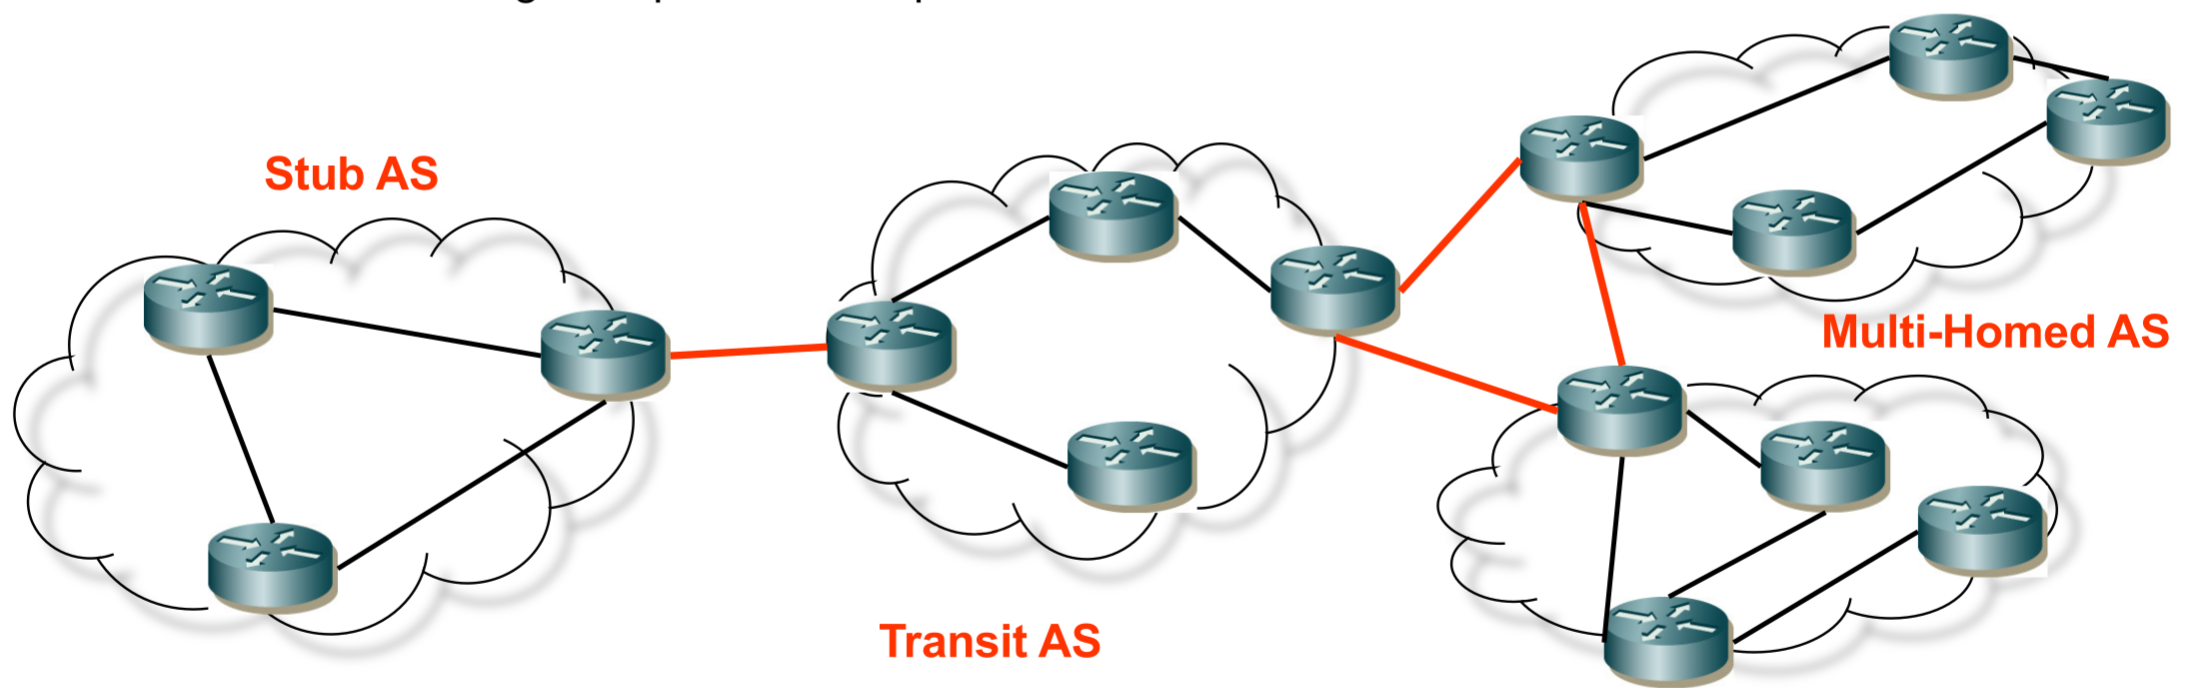
\includegraphics[width=0.9\textwidth]{images/tipologieAS.png}
    \caption{Tipologie di Autonomous Systems}
    \label{fig:tipologieAS}
\end{figure}

Lo scambio di informazioni BGP può avvenire anche tra router interni dello stesso AS; è possibile distinguerli:
\begin{itemize}
    \item \textbf{EBGP}: External BGP, scambio di informazioni tra router di frontiera di AS diversi
    \item \textbf{IBGP}: Internal BGP, scambio di informazioni tra router di frontiera dello stesso AS
\end{itemize}
Ogni AS ha un identificativo unico, l'Autonomous System Number(ASN).
\subsubsection{Approccio Path Vector}
Il BGP utilizza un approccio path vector, in cui ogni router mantiene una tabella di routing che contiene le informazioni sui percorsi verso le destinazioni e i rispettivi attributi.
Queste informazioni vengono scambiate tra i router BGP per costruire una visione globale della rete e determinare il percorso migliore per raggiungere le destinazioni.
\paragraph{Attributi BGP}
Gli attributi BGP sono informazioni associate ai percorsi che vengono utilizzate per prendere decisioni di routing. Alcuni degli attributi più comuni includono:
\begin{itemize}
    \item \textbf{AS Path}: elenca gli Autonomous Systems attraversati dal percorso
    \item \textbf{Next Hop}: indica il prossimo router da raggiungere per il percorso
\end{itemize}
Tra le diverse rotte si sceglie quella con AS-PATH più breve; in caso di rotte
con stesso costo, si sceglie quella con NEXT-HOP più vicino; in ultima istanza
ci si basa sugli altri attributi in relazione alla policy adottata.

Inoltre un router può accettare o meno gli annunci che gli giungono in base alle sue
policy.